\documentclass[12pt,notitlepage,oneside]{report}

\usepackage{buetcseugthesis}
\usepackage{bm}
\usepackage{relsize}
\usepackage{multirow}
\usepackage{enumitem}
\setlist[enumerate]{itemsep=0mm}
\newcommand\tab[1][.5cm]{\hspace*{#1}}
% Uncomment the following line if you need to write in Bangla
% \usepackage{usebangla}

% Uncomment any of the following lines should you need to
% suppress the LOF, or LOT or LOA

% \suppresslistoffigures 
% \suppresslistoftables
% \suppresslistofalgorithms

% For index creation, comment this out if you do not want to create an
% index
\makeindex[intoc]

\begin{document}

% Edit as needed below this line
% %%%%%%%%%%%%%%%%%%%%%%%%%%%%%%%%%%%%%%%%%%%%%%%%%%%%%%%%

% Chapter-1 Introduction
\chapter{Introduction}\label{intro}
The frequency of data access at the users' end has been increased by a large number for the past few years. To ensure low latency at the users' end, it is preferable to reside the data as close to the users as possible. Moreover, in present world data privacy has been a great concern and almost all the nations require the data of their citizens not to reside in some place across their national border. Now its a big concern to maintain privacy regulations and keep foreign countries from being able to subpoena data. To mitigate these two issues, almost all the companies have been building their data centers all around the world. As a result, the sparsity of data has been increased by a huge amount during the last few years.

On the other hand, the amount of data generating in present world is quite large. This huge volume has introduced  a new term ``Big Data". In general ``Big Data" is nothing but the large volume of data that can be both structured and unstructured. The excessive use of social media, scientific instruments, portable devices, sensors are the main reason behind the generation of big data. Data analysis, capture, curation, search, share, storage, transfer, visualization, query, updating, information privacy everything associated with big data has been the challenges of the present world. In case of big data the can be both wide and tall that means the dimension of the data can be quite large. As a result available techniques might not be able to perform the data analysis with the provided limited hardware. Therefore, we need  approaches that have the property of scalability.

For researchers, however, big data brings new sets of challenges like how to efficiently and effectively handle big data in commodity computers, how to apply conventional
algorithms, how
to properly manage big data in distributed setting etc. Specially, in field of
Machine Leaning and
Pattern Recognition, big data poses a threat, because the conventional algorithms
were designed
solely to fulfil its purpose where entire dataset can fit in memory. Distributed
setting was not
taken into consideration. In a nutshell, to extract any meaningful insight from this
big data, we
need powerful tools to analyse it, elastic frameworks to cope up with its sheer
volume and most
importantly we have to rethink and redesign existing algorithms which are most
suitable for
smaller sized dataset and do not take advantage of clusters.
In this thesis, we consider one kind of the machine learning algorithms, namely Probabilistic Principal Component Analysis(PPCA) and try to make it practically usable in analysing tall and wide big data which are distributed throughout the whole world. In this chapter we provide the motivation behind our research in Section \ref{sec:1}, we discuss the advantages of using PPCA in Big Data Analysis in Section \ref{sec:2}, in Section \ref{sec:3} we present our contribution in data analysis field and in Section \ref{sec:4} we briefly describe the organization of this book. 

\section{Motivation}
	\label{sec:1}
Let us assume some scenario. Let us assume that We have good availability of  machine learning models to do various kinds of data analytics. Moreoevr, our data is of the size $10000 \times 200$. That means it contains $10000$ sample which each sample has $200$ features. The machine learning models will be capable to fit such data pretty easily. As soon as the data usage and data generation rate increases the data size gets larger to $200000 \times 2000$. This time the machine learning models fails to fit such higher dimensional data. Fortunately, we have Principal Component Analysis (PCA) technique to reduce the dimensionality of the data. Thus we can get $100$ principal components from the data. Now the data is compressed enough to fit in our Machine learning models. But if the dimension of data become more higher like in millions or billions then such Tall and Wide data will neither be suitable to fit in machine learning models nor the tradition PCA algorithms can handle such large dimensional data. More question arise if the data get to be geographically distributed. We were intended to give such a method that can answer all these questions and hence solve the problems of geographically distributed higher dimensional Tall and Wide Data.

\section{Probabilistic PCA (PPCA) on Big Data}
	\label{sec:2}
As PPCA incorporates both probabilistic model of data and EM algorithm for deriving the parameters, it has some advantages from from both sides. Here we elaborate the major ones:
\begin{itemize}
	\item Firstly and most importantly, EM algorithm for deriving the parameter is computationally efficient, if only few principal components are required. If we want only $k$
	components, where $k << D$ and size of data is $N \times D$, time complexity of PPCA is $O(NDk)$. It does not require to calculate a big dense data covariance matrix as intermediate data, so communication complexity is also less. Calculating data covariance matrix
	is costly in terms of both computational and communication complexity. For this reason.
	deterministic PCA methods (like EVD, SVD) do not scale well with data (time complexity: $O(ND^2))$. More detailed analysis can be found in the technical report \cite{bishop}. Thus
	EM steps in PPCA give a well scalable algorithm and is a great advantage for big data
	analysis.
	\item For large dataset, it is very common that some entries of data can be missing. As big data
	can have missing values, deterministic PCA algorithm will give erroneous result and will
	not be suitable. But for PPCA it is not a problem. Since iterative method of PPCA uses
	expectation maximization, projected data or expected values of latent variable can still
	be derived even if some values are missing in random. This benefit of handling missing
	values is one of the major advantages of PPCA.
	\item Deterministic PCA methods are not aware of the isotropic noise that is considered by
	PPCA. It is because these methods consider the squared distance of the new data points
	from their projections into the principal subspace. So, even for data points that are ran-
	domly far from the training data, conventional PCA will give a low reconstruction cost
	if these points are close to the principal subspace. We do not face similar problems in
	PPCA as it takes ‘noise’ as a parameter and assigns likelihood accordingly.
	
	\item For a well defined problem, target dimension k can be known beforehand. But in many
	
	data reduction problems the optimal It may not be known in advance. Thus we need such
	
	a method that can find dimensionality of the principal subspace automatically from the
	
	data. This can be done by a Bayesian treatment of PCA and PPCA forms the basis for it.
	
	This is a great advantage for unsupervised learning.
	
	\item As we are deriving parameters of a probabilistic model of data, we can easily generate
	`synthesized' or `fantasy data from the distribution.
	
	\item We can combine multiple PPCA models as a probabilistic mixture for complex models to get better accuracy. Using EM algorithm we can easily train mixtures of PPCA models.
	
	\item Number of independent parameters in PPCA model grows only linearly with dimension of data D for a fixed target dimension k. Because of this reason, number of independent parameters for multivariate Gaussian distribution can be restricted while still allowing if to capture the dominant correlation in data.
	
	\item Lastly, PPCA can be applied to classification problems because we can use it to model class-conditional densities.
	\end{itemize}

\newpage
\section{Contribution}
	\label{sec:3}
Summarizing, our main contributions are:
\begin{itemize}
\item We propose an approach of PPCA that deals with geographically distributed Tall and Wide Big Data and provide an in-depth study of the relative merits against recent efficient approach \textit{sPCA} \cite{elgamal}.
\item We propose a system that builds upon Apache Spark  \cite{spark} environment and extends their functionality to support multiple data clusters learning applications.
\item We propose an apparently time efficient method to accumulate partially generated results in various data clusters.
\item Our proposed approach  will minimize the number of transfers among data centers thus minimize the inter data center bandwidth utilization.
\item Our method will be scalable to the available hardware of the data clusters. It will allow us to handle Tall and Wide big data in commodity computers even with memory of $6/8GB$.
\item We will present our experimental results implemented on the clusters in our undergraduate thesis laboratory that will justify the validity of our method.
\end{itemize}

\section{Organization of this Book}
	\label{sec:4}
	The rest of the book is organized as follows. In Chapter \ref{c:2}, we define some basic terminologies. In Chapter \ref{c:3}, we describe all the mathematical background characteristics of PCA. In Chapter \ref{c:4}, we write about our focus. In Chapter \ref{c:5}, we describe our preliminary works on regression analysis. In Chapter \ref{c:6}, we describe our main approach to solve the existing problem. Chapter \ref{c:7} describes the properties of our approach while Chapter \ref{c:8} gives a brief on our  Spark implementation. With showing the experimenta;l results in Chapter \ref{c:9}, the book concludes with Chapter \ref{c:10}. 

\endinput
%\chapter{Introduction}\label{intro}

This chapter is for your introduction.

\section{Cross Referencing}
We have incorporated the \verb@\cref@ or \verb@\Cref@ command from
\texttt{cleveref} package in this system. This will automatically
insert words like Figure, Table etc.\ in your text.

See these examples:
\begin{itemize}
\item \Cref{fig:sample} is a sample figure.
\item \Cref{tab_our} is a table.
\item \Cref{sec:cite} in \Cref{ch:citations} shows some examples of
  citations.
\end{itemize}

\section{How to Write a Section}

This is for writing section.

\section{How to Add Table and Figures}\label{contribution}
You should refer a figure as, ``\Cref{fig:sample} is a sample
figure''.

\begin{figure}[!tb]
  \centering
  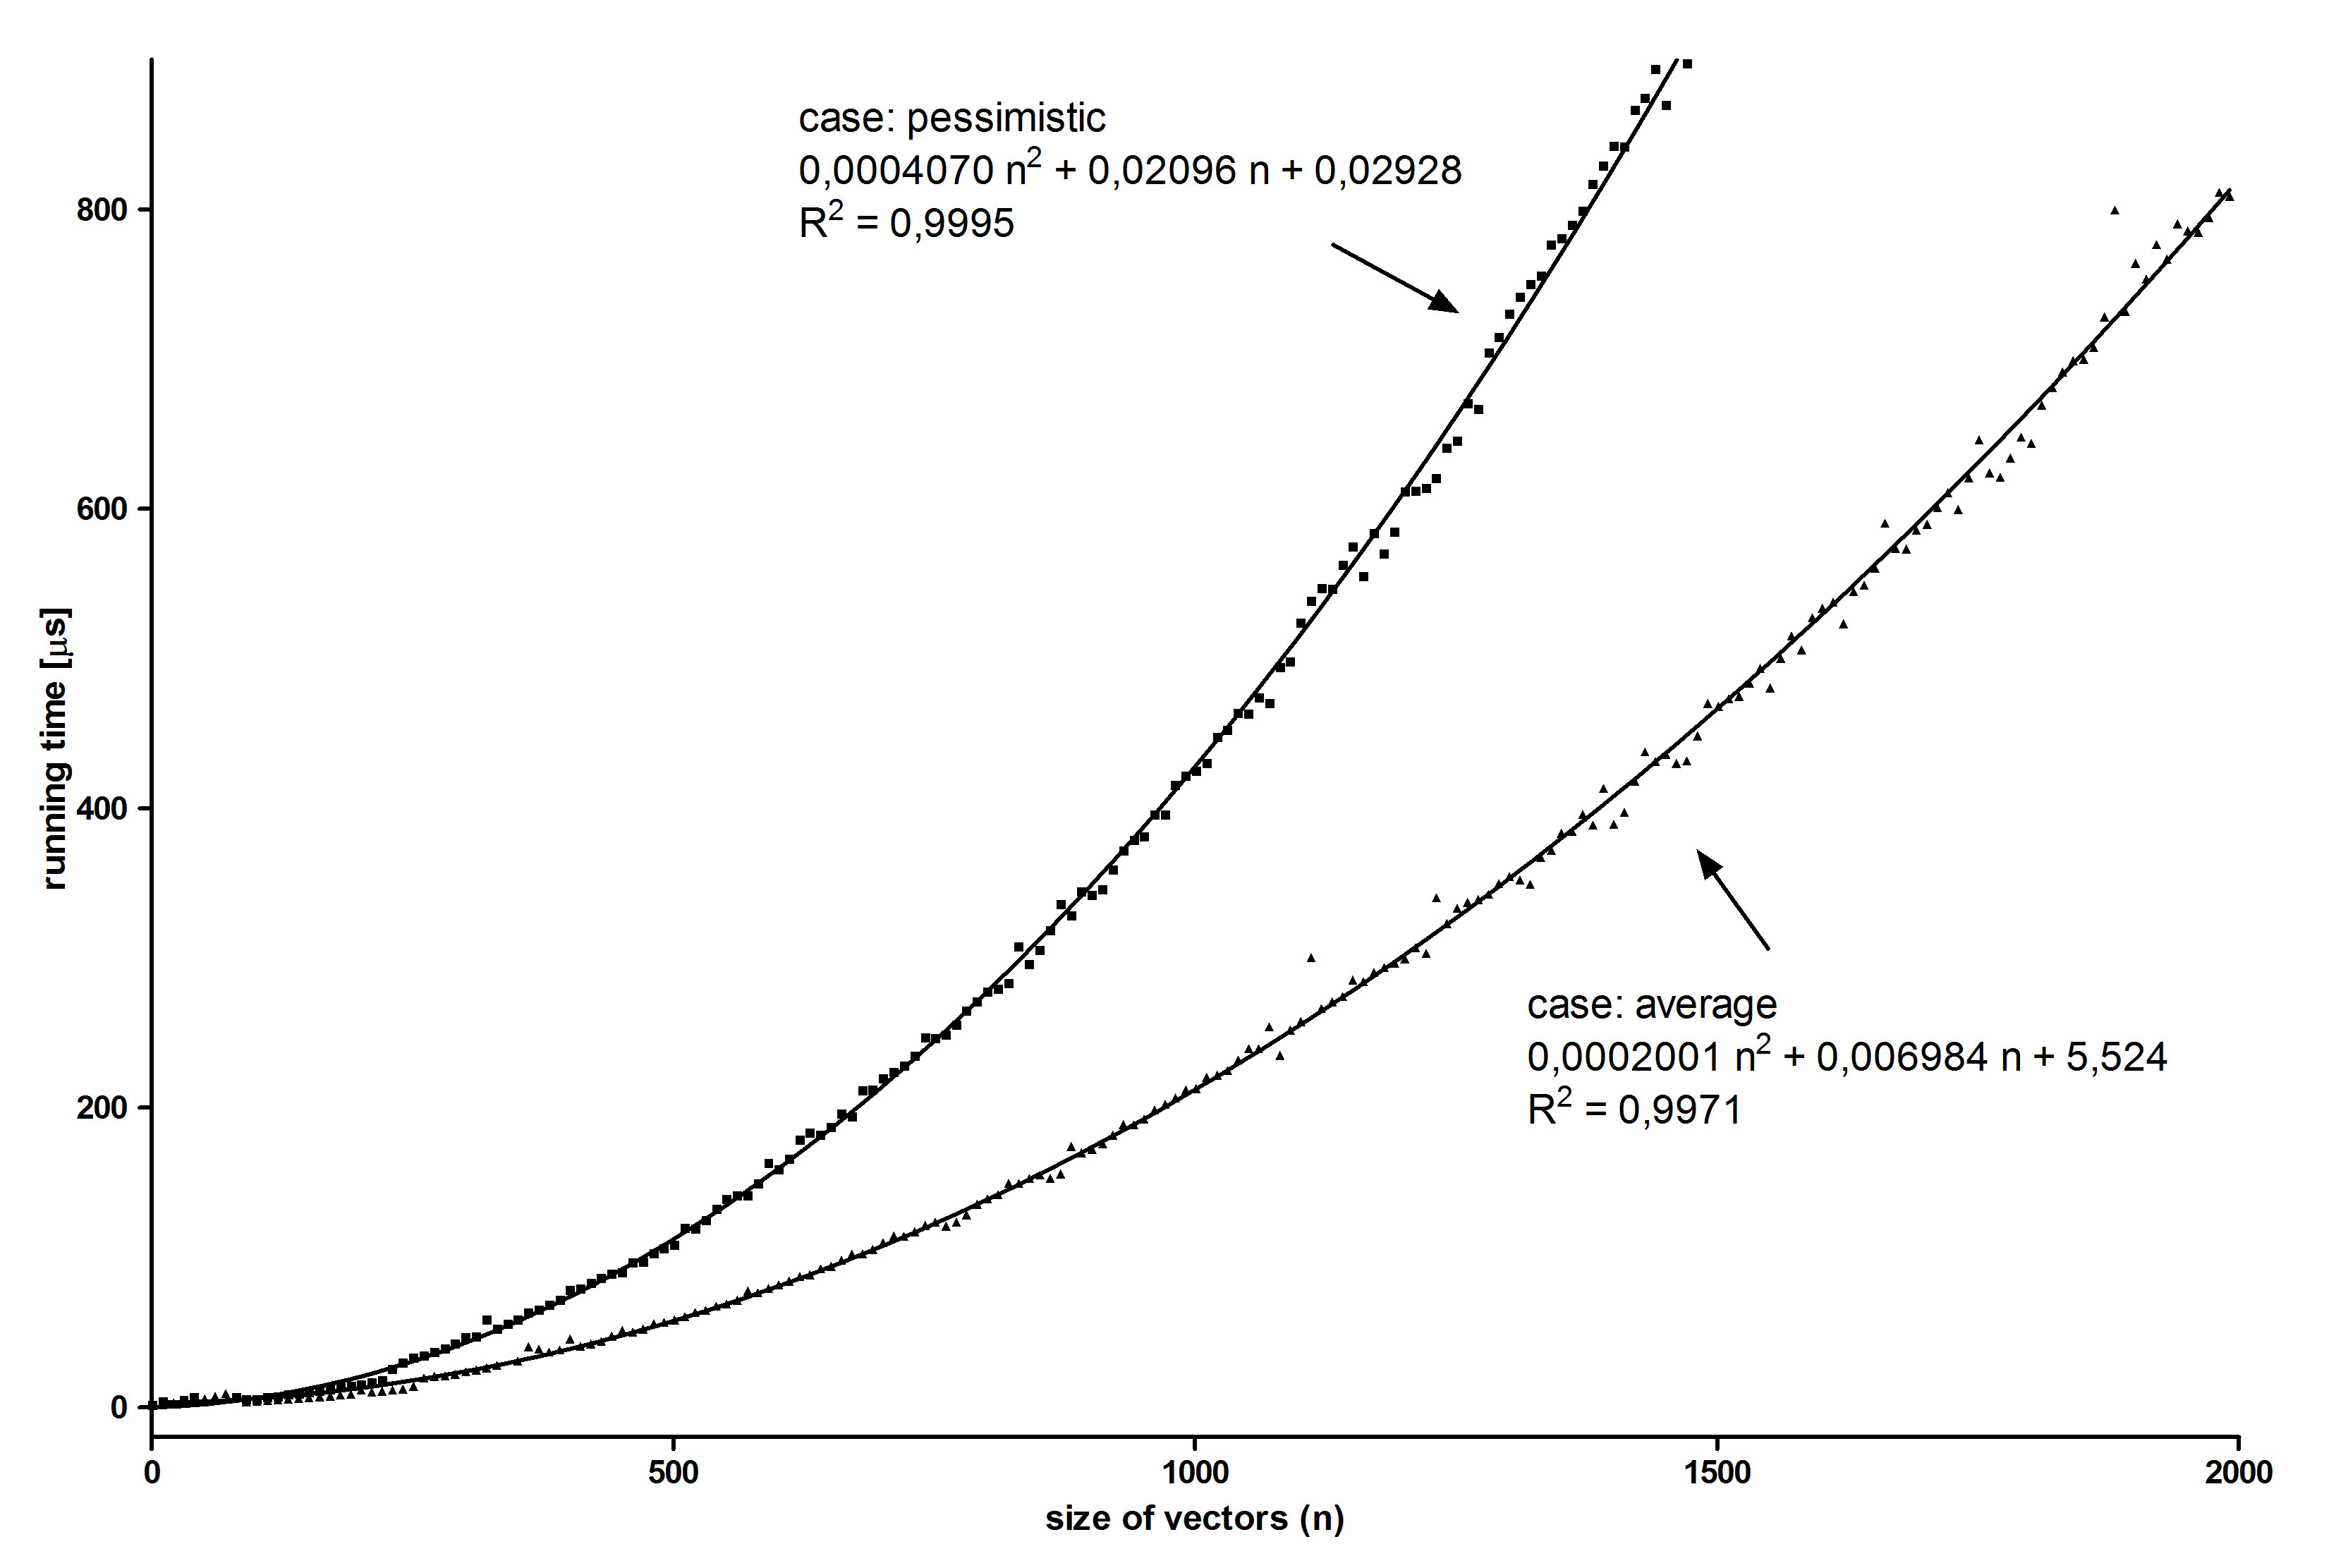
\includegraphics[width=0.9\textwidth]{figures/sample}
  \caption{This is a sample figure.}
  \label{fig:sample}
\end{figure}

				
Then we applied same test cases to our modified algorithm i.e.\ the
heuristic algorithm with our new operation \textit{Block Reversal}. The
performance is shown in \Cref{tab_our}.


\begin{table}[!tb]
  \begin{center}
    \caption{Performance table of \emph{Block reversal} in a heuristic algorithm}
    \label{tab_our}

    \begin{tabular}{|l|r|r|r|r|r|r|r|r|r|r|r|r|r|}
      \hline
      $\alpha$     & $\alpha n$ & \multicolumn{11}{c|}{Test Cases} & \multicolumn{1}{c|}{Average \# of}                                     \\
      \cline{3-13} &            & 1                                & 2  & 3  & 4  & 5  & 6  & 7  & 8  & 9  & 10 & 11 & calculated operation \\
      \hline
      0.1        & 2          & 2                                & 2	& 2  & 2  & 2  & 2  & 2  & 2  &	2  & 2	& 2  & 2                    \\
      0.2        & 4          & 4                                & 4	& 5  & 2  & 4  & 4  & 4  & 4  &	2  & 4	& 4  & 3.73                 \\
      0.3        & 6          & 5                                & 6	& 6  & 6  & 6  & 7  & 6  & 5  &	6  & 6	& 6  & 5.91                 \\
      0.4        & 8          & 7                                & 8	& 5  & 6  & 7  & 6  & 6  & 7  &	8  & 8	& 7  & 6.82                 \\
      0.5        & 10         & 9                                & 10	& 6  & 12 & 10 & 8  & 10 & 10 &	7  & 7	& 10 & 9                    \\
      0.6        & 12         & 9                                & 12	& 16 & 10 & 12 & 12 & 9  & 11 &	12 & 9	& 12 & 11.27                \\
      0.7        & 14         & 13                               & 7	& 18 & 15 & 14 & 8  & 13 & 11 &	13 & 13	& 14 & 12.64                \\
      0.8        & 16         & 10                               & 17	& 14 & 16 & 13 & 16 & 13 & 11 &	13 & 17	& 13 & 13.91                \\
      0.9        & 18         & 14                               & 16	& 15 & 12 & 15 & 11 & 15 & 11 &	15 & 12	& 12 & 13.45                \\
      1          & 20         & 18                               & 11	& 13 & 11 & 13 & 15 & 17 & 17 &	13 & 18	& 12 & 14.36                \\
      \hline
    \end{tabular}
  \end{center}
\end{table}


These are some dummy text used as page fillers only.

Lorem ipsum dolor sit amet, consectetur adipiscing elit. Cras et
ultricies massa. Nulla a sapien lobortis, dignissim nibh in, aliquet
mauris. Integer at dictum metus. Quisque in tortor congue ipsum
ultricies tristique. Maecenas ut tortor dapibus, sagittis enim at,
tincidunt massa. Ut sollicitudin sagittis ipsum, ac tincidunt quam
gravida ac. Nullam quis faucibus purus. Aliquam vel pretium
turpis. Aliquam a quam non ex interdum sagittis id vitae quam. Nullam
sodales ligula malesuada maximus consequat. Proin a justo eget lacus
vulputate maximus luctus vitae enim. Aliquam libero turpis, pharetra a
tincidunt ac, pulvinar sit amet urna. Pellentesque eget rutrum diam,
in faucibus sapien. Aenean sit amet est felis. Aliquam dolor eros,
porttitor quis volutpat eget, posuere a ligula. Proin id velit ac
lorem finibus pellentesque.

Maecenas vitae interdum mi. Aenean commodo nisl massa, at pharetra
libero cursus vitae. In hac habitasse platea dictumst. Suspendisse
iaculis euismod dui, et cursus diam. Nullam euismod, est ut dapibus
condimentum, lorem eros suscipit risus, sit amet hendrerit justo
tortor nec lorem. Morbi et mi eget erat bibendum porta. Ut tristique
ultricies commodo. Nullam iaculis ligula sed lacinia ornare.

Sed ultricies cursus nisi at vestibulum. Aenean laoreet viverra
efficitur. Ut eget sapien lorem. Mauris malesuada, augue in pulvinar
consectetur, ex tortor tristique ligula, sit amet faucibus metus
lectus interdum nisl. Nam eget turpis vitae ligula pulvinar bibendum a
ut ipsum. Mauris fringilla lacinia malesuada. Fusce id orci
velit. Donec tristique rhoncus urna, a hendrerit arcu vehicula
imperdiet. Integer tristique erat at gravida condimentum. Sed ornare
cursus quam, eget tincidunt enim bibendum sed. Aliquam elementum
ligula scelerisque leo sagittis, quis convallis elit dictum. Donec sit
amet orci aliquam, ultricies sapien nec, gravida nisi. Etiam et
pulvinar diam, et pellentesque arcu. Nulla interdum metus sed aliquet
consequat.

Proin in mi id nulla interdum aliquet ac quis arcu. Duis blandit
sapien commodo turpis hendrerit pharetra. Phasellus sit amet justo
orci. Proin mattis nisl dictum viverra fringilla. Interdum et
malesuada fames ac ante ipsum primis in faucibus. Curabitur facilisis
euismod augue vestibulum tincidunt. Nullam nulla quam, volutpat vitae
efficitur eget, porta sit amet nunc. Phasellus pharetra est eget urna
ornare volutpat. Aenean ultrices, libero eget porttitor fringilla,
purus tortor accumsan neque, sit amet viverra felis tortor eget
justo. Nunc id metus a purus tempus euismod condimentum non lacus. Nam
vitae diam aliquam, facilisis diam quis, pharetra nunc. Nulla eget
vestibulum tellus, ut cursus tellus. Vestibulum euismod pellentesque
sodales.

Maecenas at mi interdum, faucibus lorem sed, hendrerit nisi. In vitae
augue consequat diam commodo porta sit amet eu purus. Mauris mattis
condimentum feugiat. Nulla commodo molestie risus vitae maximus. Proin
hendrerit neque malesuada urna laoreet convallis. Etiam a diam
pulvinar, auctor sem ac, hendrerit risus. Ut urna urna, venenatis ac
tellus non, scelerisque tristique ligula. Vestibulum sollicitudin vel
leo malesuada accumsan. Donec sit amet erat diam. Vestibulum ante
ipsum primis in faucibus orci luctus et ultrices posuere cubilia
Curae; Vivamus odio dui, scelerisque et lorem egestas, posuere
ullamcorper nunc. Integer varius nunc nec velit tincidunt
commodo. Mauris rhoncus ultrices sapien non suscipit.


End of dummy text.


\endinput

%Chapter-2 Basic Terminologies

\chapter{Basic Terminologies}
	\label{c:2}
\section{Big Data}
Big Data is a term for voluminous amounts of data that has the potential to be mined for information. Big data can be analyzed for insights that lead to better decisions. Big Data is characterized by three main factors: the extremely large volume of data, the wide variety of data types and the velocity at which the data must be processed. 

Such voluminous data can come from countless different sources such as business sales records, the collected results of scientific experiments of real-time sensors used in the internet of things (IoT).

Data may exist in wide variety of types, including structured data, such as SQL database stores, as well as unstructured data such as document files or streaming data from sensors. Big data of different types and from different sources may be used together during analysis.

Principal Component Analysis(PCA), which is the main focus of our thesis, is considered as a pre-processing step in Big Data Analytic. It reveals the relations between the different dimensions of data and allows a reduction in dimensionality of the data via low rank approximation.

\section{Data Analysis}
According to \cite{dataanalysis} Data analysis, also known as analysis of data or data analytics, is a process of inspecting, cleansing, transforming, and modeling data with the goal of discovering useful information, suggesting conclusions, and supporting decision-making. Data analysis has multiple facets and approaches, encompassing diverse techniques under a variety of names, in different business, science, and social science domains.

Data mining is a particular data analysis technique that focuses on modeling and knowledge discovery for predictive rather than purely descriptive purposes, while business intelligence covers data analysis that relies heavily on aggregation, focusing on business information \cite{01}. In statistical applications data analysis can be divided into descriptive statistics, exploratory data analysis (EDA), and confirmatory data analysis (CDA). EDA focuses on discovering new features in the data and CDA on confirming or falsifying existing hypotheses. Predictive analytics focuses on application of statistical models for predictive forecasting or classification, while text analytics applies statistical, linguistic, and structural techniques to extract and classify information from textual sources, a species of unstructured data. All are varieties of data analysis.


\section{Data Analysis Approaches }
Under these circumstances, we can see that in case of extracting some information from the existing data, we may have to cover a good number of data centres located at different geographical area. This has given the introduction of a new data analysis approach, ``Distributed Data Analysis''. Therefore we get the idea of two approaches of data analysis.

\subsection{Centralized Approach}
The centralized approach to data analysis from distributed data centers is to centralize them first. As shown in Figure \ref{centralized}, this involves a two different steps: 


\begin{enumerate}

\item \textbf{Centralizing step} Data from various data centers are copied into a single data center. It involves recreation of data of all data centers in one location.

\item \textbf{Analysis Step} Process of extracting the necessary information from the centralized data takes place in that single data center. Here traditional intra data center technology is sufficient for the analysis purpose.

\end{enumerate}

\begin{figure}[!htbp]
  \centering
	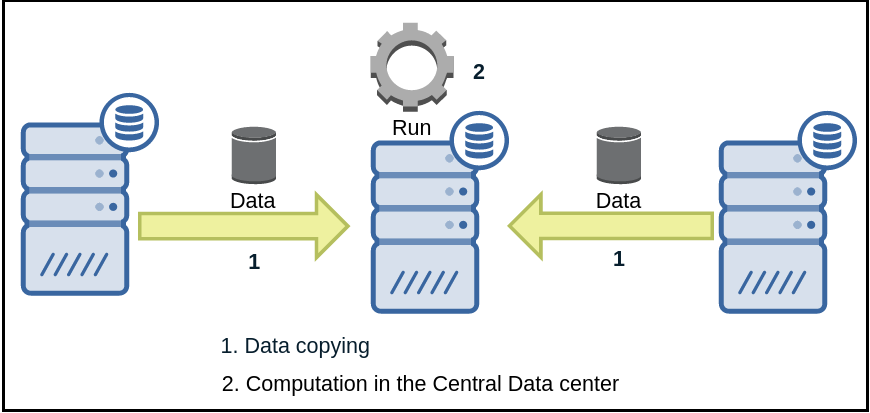
\includegraphics[width=3.2in]{figures/1.png}
	\caption{Centralized Approach}
	\label{centralized}
\end{figure}


This centralized approach is predominant in most practical settings. 
There are mainly two reasons behind its popularity. 
\begin{enumerate}
\item There are lots of frameworks that have already been established for centralized learning approach. That is why centralizing the data is the easiest way to reuse existing data analysis frameworks \cite{1,2,3}
\item Learning algorithms are highly communication intensive. Thus it is assumed that they will note be properly responsive to cross data center execution.
\end{enumerate}
For these reasons, this centralized approach is consistent with reports on the infrastructures of other large organizations, such as Facebook \cite{4}, Twitter \cite{5}, and LinkedIn \cite{6}. 

However the centralized approach has two shortcomings.
\begin{enumerate}
\item While making multiple copy of data at the central data center, it consumes a good amounts of inter data center bandwidth. Since inter data center bandwidth is expensive, it is not easy to increase it according to the necessity \cite{7,8,9,10}.
\item While creating copy of data, it may be a case that data is crossing national borders. However, in current workd data sovereignty is a growing concern that might create a big limitation in this aspect \cite{11,12}.

\end{enumerate}

\subsection{Distributed Approach}
In the distributed approach, raw data is kept in their corresponding data centers. Every data center does a portion of the execution that is only on the data of that data center. The final analysis takes pales by passing small amount of information among the data centers. 

\begin{figure}[!htbp]
  \centering
	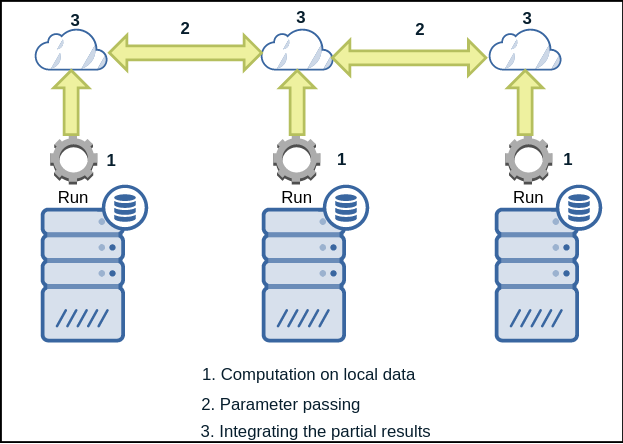
\includegraphics[width=3.2in]{figures/2.png}
	\caption{Distributed Approach}
\label{distributed}
\end{figure}

So according to Figure \ref{distributed}, we can see this approach includes three steps:

\begin{enumerate}
\item \textbf{Local Computation} Whenever the command of starting of any learning process is issued every data center start a partial computation on its own data. They create necessary high level information on data that will be needed in the final computation.

\item \textbf{Parameter Passing} Data centers communicate among themselves and share valuable information.

\item \textbf{Final Computation} By integrating the partial results data centers make the final computational model.
\end{enumerate}

In this way distributed solutions can achieve much lower cross data centers bandwidth utilization, and thus substantially lower cost for large-scale analysis tasks. As the current world has got a concern about `Big Data' and `Data Sovereignty', the distributed approach seems to be more efficient. 


\section{Geo Distributed Data}

Over the year concept about data has changed a lot. Only few years ago data were generated locally and computation was done locally also. But now data are generated over the whole world. Data are not bound to locality. 

Data are by born geographically distributed over the world. That's why nowadays geo distributed analysis is being popular. Data are not gather in one place rather algorithms are being designed to run over the geo-distributed data.

\section{Data Sovereignty}

Data sovereignty is the concept that information which has been converted and stored in binary digital form is subject to the laws of the country in which it is located \cite{sovereign}.

Many of the current concerns that surround data sovereignty relate to enforcing privacy regulations and preventing data that is stored in a foreign country from being subpoenaed by the host country's government.

The wide-spread adoption of cloud computing services, as well as new approaches to data storage including object storage, have broken down traditional geopolitical barriers more than ever before. In response, many countries have regulated new compliance requirements by amending their current laws or enacting new legislation that requires customer data to be kept within the country the customer resides. 

Verifying that data exists only at allowed locations can be difficult. It requires the cloud customer to trust that their cloud provider is completely honest and open about where their servers are hosted and adhere strictly to service level agreements (SLAs).


\section{Data Cluster and Cluster Computing}
A cluster is a system comprising two or more computers or systems (called nodes) which work together to execute a particular task. They are usually deployed for High Availability (HA) for greater reliability and High performance Computing (HPC) to provide greater computational power than a single computer can provide.

The components of a cluster are usually connected to each other through fast local area networks (LANs), with each node running its own instance of an operating system(OS). In most circumstance, all of the nodes use the same hardware and the same OS, although it is possible to user different OS and/or different hardware on each computer.

\subsection{Advantages}

Cluster computing provides the following important advantages.

\begin{enumerate}
	\item Cluster computing is completely a scalable solution. Resources may be removed or new resources may be added to clusters after the system has already been deployed. They can scale to very large and complex systems with large computing power, not possible with single computers. Also each of the machines in a cluster can be a complete system, usable for a Wide range of other computing applications.
	
	\item Clustering solutions are more fault tolerant. If one of the servers in the system stops working, other servers in the cluster can take the load. If a server in the cluster needs any maintenance, it can be done by stopping it while handing the load over to other servers.
	
	\item Clusters are more cost effective. A cluster will cost much less than a single computer of comparable speed and availability.
	
\end{enumerate}

\subsection{Disadvantages}

Unfortunately, clustering suffers from some limitations as well:

\begin{enumerate}
	\item As clusters consist of many computers running in parallel, it is obvious that these systems are only efficient in carrying out a specific task if the task can be separated into smaller subtasks that can be completed in parallel. This may not always be possible.
	
	\item The network hardware used to communicate typically has low bandwidth and high latency (as compared to the link between the different processors in a single computer) and this communication complexity usually acts as the bottleneck during execution of a task. Thus, algorithms are required to be designed to run on distributed settings and must be optimized to reduce communication between nodes which may be tough to do.
	
	\item Clusters can become very large and complex, and the maintenance of these large and complex systems could be quite expensive.
\end{enumerate}

\section{Data Parallelism}
Data parallelism is a form of parallelization across multiple processors in parallel computing environments. It focuses on distributing the data across different nodes, which operate on the data in parallel. It can be applied on regular data structures like arrays and matrices by working on each element in parallel. It contrasts to task parallelism as another form of parallelism \cite{dparallel}.

A data parallel job on an array of `$n$' elements can be divided equally among all the processors. Let us assume we want to sum all the elements of the given array and the time for a single addition operation is Ta time units. In the case of sequential execution, the time taken by the process will be $n*Ta$ time units as it sums up all the elements of an array. On the other hand, if we execute this job as a data parallel job on 4 processors the time taken would reduce to $(n/4)*Ta$ + Merging overhead time units. Parallel execution results in a speed up of $4$ over sequential execution. One important thing to note is that the locality of data references plays an important part in evaluating the performance of a data parallel programming model. Locality of data depends on the memory accesses performed by the program as well as the size of the cache.

\section{Model Parallelism}

Data Parallelism and Model Parallelism are different ways of distributing an algorithm. These are often used in the context of machine learning algorithms that use stochastic gradient descent to learn some model parameters \cite{mparallel}.

In model parallelism algorithm sends the same data to all the cores. Each core is responsible for estimating different parameter(s). Cores then exchange their estimate(s) with each other to come up with the right estimate for  all the parameters.


\section{TensorFlow}

TensorFlow \cite{tensor} is an open source software library for numerical computation using data flow graphs. As we have used the concept of model parallelism and data parallelism in our geo distributed algorithm, so it is important. Because in \textit{TensorFlow}  architecture both the model parallelism and data parallelism have been used.

The flexible architecture of \textit{TensorFlow} allows to deploy computation to one or more CPUs or GPUs in a desktop, server, or mobile device with a single API. \textit{TensorFlow} was originally developed by researchers and engineers working on the \textit{Google} Brain Team within \textit{Google}'s Machine Intelligence research organization for the purpose os conducting machine learning and deep neural networks research, but the system is general enough to be applicable in wide variety of other domains as well.


\section{\textit{Hadoop} Cluster}
\textit{Hadoop} \cite{116} is an open source software framework built on two technologies, Linux operation system and Java programming language. It supports the processing and storage of extremely large data sets in a cluster computing environment. It is part of the Apache project sponsored by the Apache Software Foundation.

All the modules in \textit{Hadoop} are designed with the assumption that hardware failures are common occurrences and should be automatically handled by the framework. 

\section{\textit{Hadoop} MapReduce}
MapReduce is the heart of \textit{Hadoop}. MapReduce is a processing technique and a programming paradigm for distributed computing based on Java. It allows for massive scalability across hundreds or thousands of servers in a \textit{Hadoop} cluster.

The MapReduce algorithm consists of two important tasks, namely Map and Reduce. Map takes a set of data and converts it into another set of data, where individual elements are broken down into tuples (key-value-pairs). Reduce takes the output from a map as an input and combines those data tuples into smaller set of tuples. As the sequence of the name MapReduce implies, the reduce task is always performed after the map job.

During a MapReduce job, \textit{Hadoop} assigns the Map and Reduce tasks to the appropriate serves in the cluster. The framework manages all the details of data passing such as issuing tasks, verifying task completion, and copying data around the cluster between the nodes.

Most of the computing takes place on nodes with data on local disks that reduces the network traffic.

After completion of the given tasks, the cluster collects and reduces the data to form an appropriate result, and sends it back to the \textit{Hadoop} server.

\section{Spark Cluster}
Spark \cite{spark} is an open source processing engine that provides scalable, massively parallel, in-memory execution environment for running analytics applications. It can be thought as an in-memory layer that sits above multiple data stores, where data can be loaded into memory and analyzed in parallel across a cluster.

Much like MapReduce, Spark works to distribute data across a cluster, and process that data in parallel. But unlike MapReduce - which shuffles files around on disk - Spark works in memory, making it much faster at processing data than MapReduce.

Spark includes rebuilt machine-learning algorithms and graph analysis algorithms that are especially written to execute in parallel and in memory. It also supports interactive SQL processing of queries and real-time streaming analytics.

Spark provides programmers with an application programming interface (API) centered on a data structure called the resilient distributed dataset (RDD), a read-only multiset of data items distributed over a cluster of machines, that is maintained in a fault-tolerant way. The availability of RDDs facilitates the implementation of both iterative algorithms, that visit their dataset multiple times in a loop, and exploratory data analysis (the repeated database-style querying of data). Thus, Spark is the ideal platform for implementing pragmatic PPCA (our proposed algorithm) which is an iterative algorithm.


\section{Dimensionality Reduction}

\section{Vector Norms}
A norm is a function $\pmb{||.||: V\rightarrow R}$ which satisfies

\begin{enumerate}[label={(\Roman*)}]
	\item  $\pmb{\parallel x \parallel \geq 0, \forall x \in V\ and \parallel x \parallel = 0 \Longleftrightarrow x = 0}$
	\item $ \pmb{\parallel x+y\parallel \leq \parallel x\parallel + \parallel y\parallel , \forall x,y  \in  V } $
	\item $ \pmb{\parallel \lambda x \parallel = \parallel \lambda \parallel \parallel x \parallel , \forall \lambda \in C \quad and \quad \forall x \in V}$
\end{enumerate}

Where $\pmb{V  \subseteq  C^n} $ is known as the vector space. In words, these conditions require that (I) the norm of a nonzero vector is strictly positive, (II) the norm of a vector sum does not exceed the sum of the norms of its parts which is known as the triangle inequality, and (III) scaling a vector scales its norm by the same amount. Thus, norms can be thought of as functions that define the size of a vector.

\section{p-Norm}

p-Norm is a family of vector norms, denoted as $\pmb{ \parallel . \parallel _p }$, given by:


$$\pmb{ \parallel x \parallel _p \quad} = \quad (\sum_{i=1}^{n} \pmb{|x_i|^p})^ {\pmb{\frac{1}{p}}} $$

The most widely used are the 1-norm, 2-norm (also known as Euclidean norm ), and $ \infty-norm$ ( also known as sup-norm):

\begin{align*}
 \parallel x \parallel _1 &= \sum_{i=1}^{n} |x_i| \\
 \parallel x \parallel _2 &= \sqrt{\sum_{i=1}^{n} x_i^2}\\
  \parallel x \parallel _\infty &= max(|x_i|)
\end{align*}

\section{Frobenius Norm}
This is a element-wise norm where the vector norm used is the 2-norm. Each entry of the matrix is considered as a dimension of a vector and 2-norm of the resulting vector is calculated. So we have,
$$ \pmb{\parallel A \parallel _F} = \sqrt{\sum_{i=1}^{m}\sum_{j=1}^{n}\pmb{a_{ij}^2}}$$

which is equivalent to 

$$\pmb{ \parallel A \parallel _F = \sqrt{tr(A*A)} = \sqrt{tr(AA*)} }$$


where A is an $ m x n $ matrix, $a_ij$ is the value in the i-th row and j-th column of A, A* is the conjugate transpose of A, and tr(B) is the trace of B (the sum of its diagonal entries). Since tr(AA*) is the sum of the eigenvalues of AA*, we have an alternative characterization of the Frobenius norm:

$$ \pmb{\parallel A \parallel _F }= \sqrt{\sum_{i=1}^{n}\lambda _i} $$


\section{Normal Distribution}

In probability theory, the normal (or Gaussian) distribution is a very common continuous probability distribution. Normal distributions are important in statistics and are often used in the natural and social sciences to represent real-valued random variables whose distributions are not known \cite{01} \ \ \ [2].

The normal distribution is useful because of the central limit theorem. In its most general form, under some conditions (which include finite variance), it states that averages of samples of observations of random variables independently drawn from independent distributions converge in distribution to the normal, that is, become normally distributed when the number of observations is sufficiently large. Physical quantities that are expected to be the sum of many independent processes (such as measurement errors) often have distributions that are nearly normal  \ \ \  [3]   Moreover, many results and methods (such as propagation of uncertainty and least squares parameter fitting) can be derived analytically in explicit form when the relevant variables are normally distributed.

The normal distribution is sometimes informally called the bell curve. However, many other distributions are bell-shaped (such as the Cauchy, Student's t, and logistic distributions). Even the term Gaussian bell curve is ambiguous because it may be used to refer to some function defined in terms of the Gaussian function which is not a probability distribution because it is not normalized in that it does not integrate to 1.

The probability density of the normal distribution is \cite{normal}
$$\pmb{f(x | \mu , \sigma ^ 2) = \frac{1}{\sqrt{2\pi \sigma ^2}} e^{-\frac{(x-\mu)^2}{2 \sigma ^2}} }$$

Where: 

\begin{itemize}
	\item $\mu$ is the mean or expectation of the distribution (and also its median and mode).
	\item $ \sigma $ is the standard deviation.
	\item $ \sigma ^2 $ is the variance.
\end{itemize}




\section{Matrix Diagonalization}

Matrix diagonalization is the process of taking a square matrix and converting it into a special type of matrix--a so-called diagonal matrix--that shares the same fundamental properties of the underlying matrix. Matrix diagonalization is equivalent to transforming the underlying system of equations into a special set of coordinate axes in which the matrix takes this canonical form. Diagonalizing a matrix is also equivalent to finding the matrix's eigenvalues, which turn out to be precisely the entries of the diagonalized matrix. Similarly, the eigenvectors make up the new set of axes corresponding to the diagonal matrix.

The remarkable relationship between a diagonalized matrix, eigenvalues, and eigenvectors follows from the beautiful mathematical identity (the eigen decomposition) that a square matrix A can be decomposed into the very special form

$$ A \quad = \quad PDP^{-1} $$

where P is a matrix composed of the eigenvectors of $A$, $D$ is the diagonal matrix constructed from the corresponding eigenvalues, and $P^{-1}$ is the matrix inverse of $P$. According to the eigen decomposition theorem, an initial matrix equation

$$ AX \quad = \quad Y $$

can always be written 

$$ PDP^{-1}X = Y $$

(at least as long as P is a square matrix), and premultiplying both sides by $P^{-1}$ gives

$DP^-1X = P^{-1}Y.$

Since the same linear transformation $P^{-1}$ is being applied to both X and Y, solving the original system is equivalent to solving the transformed system

$DX' = Y'$,

where $X'=P^{-1}X$ and $Y'=P^{-1}Y$. This provides a way to canonicalize a system into the simplest possible form, reduce the number of parameters from $n \times n$ for an arbitrary matrix to $n$ for a diagonal matrix, and obtain the characteristic properties of the initial matrix. This approach arises frequently in physics and engineering, where the technique is oft used and extremely powerful.



\section{Expectation Maximization (EM) Algorithm}

\section{Stop Condition}

In iterative algorithm like EM, main terminating condition considered is the change in desired variable or objective function. For example in PPCA our desired variables are $W$ and $ \sigma ^2$. To check convergence we can give tolerance limit as input. If magnitude of changes in desired variable is less than our tolerance limit then we consider our algorithm has converged. But this is not most effective when we want to know how much accuracy we have obtained after convergence. Thus in many cases, error is checked after each iteration and algorithm is terminated if error goes down our target limit.





%Chapter-3 PCA as Data Analytic Technique
\chapter{PCA as a Data Analytic Tool}
	\label{c:3}
Principal component analysis (PCA) is a statistical procedure that uses an orthogonal transformation to convert a set of observations of possibly correlated variables into a set of values of linearly uncorrelated variables called principal components \cite{13}. The number of principal components is less than or equal to the smaller of the number of original variables or the number of observations. This transformation is defined in such a way that the first principal component has the largest possible variance and each succeeding component in turn has the highest variance possible under the constraint that it is orthogonal to the preceding components. As we can use PCA for dimensionality reduction, it can be used as a preprocessing step  in many machine learning algorithms that do not perform well with high-dimensional data. Therefore we can easily realize that PCA is an excellent tool for big data analysis. 

There are several ways to perform PCA. Eigen Value Decomposition (EVD) of covariance matrix and Singular Value Decomposition (SVD) are two basic and most common ways \cite{14}. These methods usually perform better on small datasets on a single machine. But in distributed settings and for big data, they introduce a new set of difficulties; they do not scale well to high dimensional data and are inefficient in terms of computation and communication cost \cite{elgamal}. To overcome these difficulties, two other methods, Stochastic SVD (SSVD) \cite{16} and Probabilistic PCA (PPCA) \cite{17} are used in practice. But unlike the other methods to calculate principal component (i.e. EVD of covariance matrix, SVD, SSVD), PPCA has two important advantages. It has the ability of handling missing data and calculating probabilistic model to generate synthesized data \cite{18}. These features are best suited for big data as missing values are prevalent in this case and a probabilistic model of the data will be more effective for analytical purposes.

Despite of being an excellent tool of data analysis, we lack in proper approach of PPCA in big data analysis. We saw a decent approach of making scalable PCA or \textit{sPCA} in a distributed environment  \cite{elgamal}.  It was designed for data analysis on large datasets on distributed commodity clusters. But unfortunately this approach is not capable of handling datasets with very large dimension, we can say data that is at the same time tall and wide. Moreover data sovereignty is not ensured. There was no method of performing PCA on big data located at different geographic location which involves independent computation at different clusters and accumulation of intermediate results. 

In this chapter, we will try to show in depth the various approaches of performing PCA with their advantages and disadvantages. Moreover we will show the very recent optimization on scalability of PPCA which is known as \textit{sPCA} with its special features and limitations.

\section{Assumptions Involved in PCA}
Mathematically, PCA is defined as on orthogonal linear transformation that transforms the data to a new coordinate system such that the greatest variance by some projection of the data comes to lie on the first coordinate (called the first principal component), the second gratest variance on the second coordinate and so on. Therefore, the assumptions involved in PCA are:

\begin{enumerate}
\item \textbf{Linearity}\\
Linearity vastly simplifies the problem by restricting the set of potential bases. With this
assumption PCA is now limited to re-expressing the data as a linear combination of its
basis vectors that is, we need to find the appropriate change of basis.
\item \textbf{Large variances have important structure}\\
This assumption also encompasses the belief that the data has a high Signal-to-Noise
Ratio ($SNR = \dfrac{\sigma_{signal}^2}{\sigma_{noise}^2}$). Hence, principal components with larger associated variances represent interesting structure, while those with lower variances represent noise.
Note that this is a strong, and sometimes, incorrect assumption.
\item \textbf{Orthogonal PCs}\\
This assumption provides an intuitive simplification that makes PCA soluble with linear algebra decomposition techniques.  
\end{enumerate}

\section{PCA and Change of Basis}
The goal of principal component analysis is to identify the most meaningful basis to re-express a data set. The hope is that this new basis will filter out the noise and reveal hidden structure. Determining this fact allows an experimenter to discern which dynamics are important, redundant or noise. 


With this rigor we may now state more precisely what PCA asks: \textit{Is there another basis, which is a linear combination of the original basis, that best re-expresses our data set?}


Let $\pmb{X}$ be the original data set, where each column is a single sample (or moment in time) of our data set.Here $\pmb{X}$ is a $D \times N$ matrix where $\pmb{N}$ in the number of samples and $\pmb{D}$ is the dimension of each sample. Let Y be another $D \times N$ matrix related by a linear transformation $\pmb{P}$. $\pmb{X}$ is the original recorded data set and $\pmb{Y}$ is a new representation of that data set.

\begin{equation}
\label{eq1}
\pmb{Y = PX}
\end{equation}
Also let us define the following quantities
\begin{itemize}
\item
 $\pmb{p_i}$ are the rows of $\pmb{P}$
 \item
 $\pmb{x_i}$ are the columns of $\pmb{X}$ 
 \item
 $\pmb{y_i}$ are the columns of $\pmb{Y}$
\end{itemize}


%\newpage
Equation \ref{eq1} represents a change of basis and thus can have many interpretations:
\begin{itemize}
\item $\pmb{P}$ is a matrix that transforms $\pmb{X}$ into $\pmb{Y}$
\item Geometrically, $\pmb{P}$ is a rotation and a stretch which again transforms $\pmb{X}$ into $\pmb{Y}$
\item The rows of $\pmb{P}$, $\{\pmb{p_1,p_2, \dots , p_D}\}$ are a set of new basis vectors for expressing the columns of $\pmb{X}$
\end{itemize}


The latter interpretation is not obvious but can be seen by writing out the explicit dot products of $\pmb{PX}$

\begin{align*}
\pmb{PX} &= 
\left[ \begin{array}{c}
\pmb{p_1} \\
\pmb{\vdots} \\
\pmb{p_D} 
\end{array}          \right]
\left[ \begin{array}{ccc}
\pmb{x_1} &\pmb{\hdots} &\pmb{x_N} \\
\end{array}          \right]
\\\pmb{Y} &= 
\left[ \begin{array}{ccc}
\pmb{p_1\cdot x_1} & \dots &\pmb{p_1\cdot x_N} \\
\vdots & \ddots &\vdots \\
\pmb{p_D\cdot x_1} & \dots &\pmb{p_N\cdot x_N} \\
\end{array}          \right]
\end{align*}

\newpage We can note the form of each column of  $\pmb{Y}$

$$\pmb{y_i} = 
\left[
\begin{array}{c}
\pmb{p_1 \cdot x_i}\\
\pmb{\vdots}\\
\pmb{p_D \cdot x_i}
\end{array}
\right]
$$

We recognize that each coefficient of $\pmb{y_i}$ is a dot-product of $\pmb{x_i}$ with the corresponding row in $\pmb{P}$. In other words, the $j^{th}$ coefficient of $\pmb{y_i}$ is a projection on to the $j^{th}$ row of $\pmb{P}$. This is in fact the very form of an equation where $\pmb{y_i}$ is a projection on to the basis of $\{\pmb{p_1, \hdots, p_D }\}$. Therefore, the rows of P are a new set of basis vectors for representing of columns of $\pmb{X}$.

By assuming linearity the problem reduces to finding the appropriate change of basis. The row vectors $\{\pmb{p_1, \hdots, p_D }\}$ in this transformation will become the principal components of $\pmb{X}$.. Several questions now arise:

\begin{itemize}
\item What is the best way to re-express $\pmb{X}$?
\item What is a good choice of basis $\pmb{P}$?
\end{itemize}

These questions must be answered by next asking ourselves what features we would like $\pmb{Y}$ to exhibit. Evidently, additional assumptions beyond linearity are required to arrive at a reasonable result. The selection of these assumptions is the subject of the next section.



\section{Eigenvalue Decomposition (EVD)}
Given a matrix $\textbf{Y}$ of size $N \times D$ ($N$ rows and $D$ columns), a PCA algorithm obtains $d$ principal components ($d \leq D$) that explain the most variance (and hence information) of the data in matrix $\textbf{Y}$ \cite{pca,kraska}. To be useful in practice, $d$ is chosen to be much smaller than $D$, that is $d \ll D$ . In case EVD technique, the target matrix $V$ is of dimension $N \times k$ where the columns of $V$ are the principal components of $\textbf{Y}$. 

\subsection{Covariance Matrix}
How do we quantify and generalize these notions to arbitrarily higher dimensions? Consider two sets of measurements with zero means:
$$A = \{a_1,a_2,...,a_N\} , B = \{b_1,b_2,...,b_N\}$$
where the subscript denotes the sample number. The variance
of $\pmb{A}$ and $\pmb{B}$ are individually defined as,
$$\sigma_A^2 = \dfrac{1}{N}\sum_i a_i^2$$
$$\sigma_B^2 = \dfrac{1}{N}\sum_i b_i^2$$
The covariance between  $\pmb{A}$ and $\pmb{B}$ is a straight-forward generalization.
$$covariance\ of\ \pmb{A}\ and\ \pmb{B} \equiv \sigma_{AB}^2 = \dfrac{1}{N}\sum
_i a_ib_i$$
The covariance measures the degree of the linear relationship between two variables. A large positive value indicates positively correlated data. Likewise, a large negative value denotes negatively correlated data. The absolute magnitude of the covariance measures the degree of redundancy. Some additional facts about the covariance:
\begin{itemize}
\item
$\sigma_{AB}$ is zero if and only if $\pmb{A}$ and $\pmb{B}$ are uncorrelated (e.g. Figure \ref{corel}, left panel)
\item
$\sigma^2_{AB} = \sigma^2_A\ if\ A = B$
\end{itemize}


\begin{figure}[!htbp]
\centering
\frame{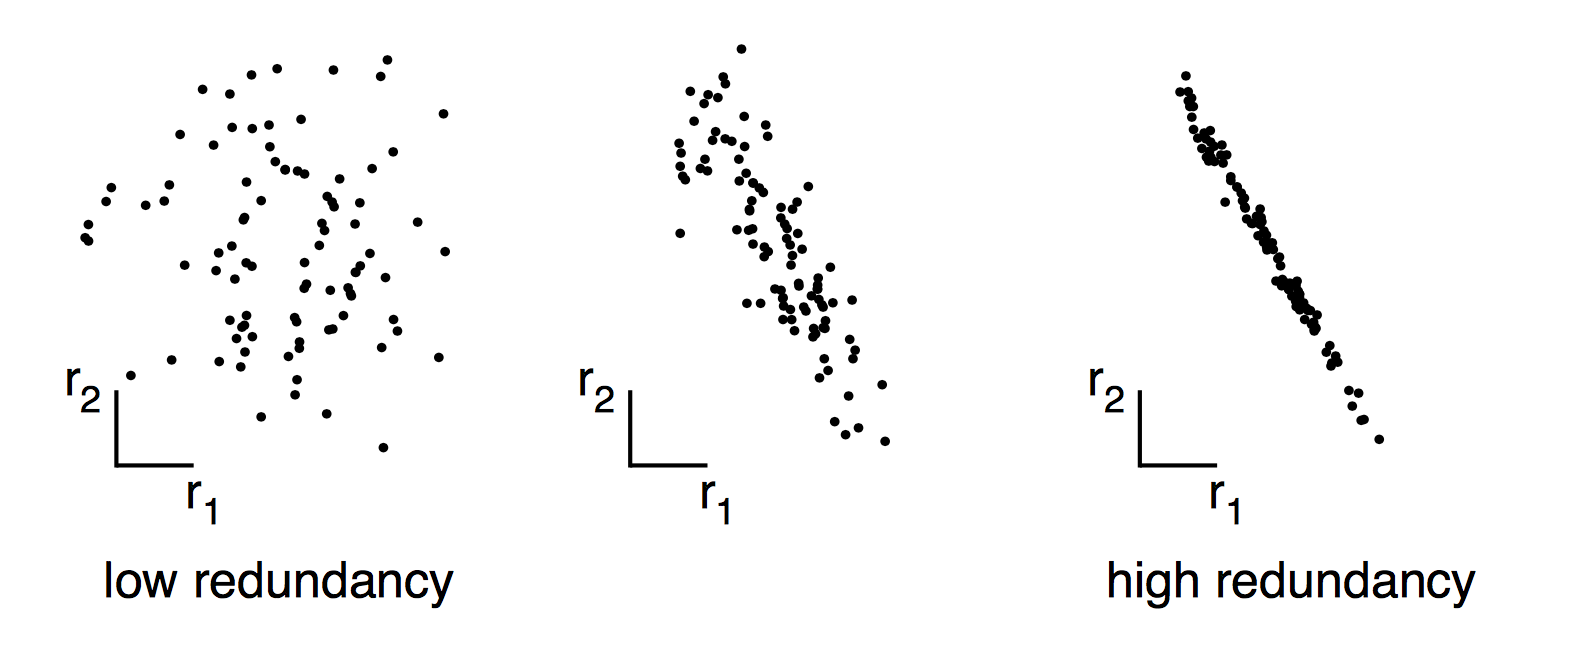
\includegraphics[scale=.5]{figures/corel}}
\caption{A spectrum of possible redundancies in data from the two separate measurements $r_1$ and $r_2$. The two measurements on the left are uncorrelated because one can not predict one from the other. Conversely, the two measurements on the right are highly correlated indicating highly redundant measurements.}
\label{corel}
\end{figure}

We can equivalently convert $\pmb{A}$ and $\pmb{B}$ into corresponding row
vectors.
\begin{align*}
\pmb{a} &= [a_1\ a_2\ \dots \ a_n]\\
\pmb{b} &= [b_1\ b_2\ \dots \ b_n]
\end{align*}
so that we may express the covariance as a dot product matrix computation
$$\sigma_{ab}^2 \equiv \dfrac{1}{N}\pmb{ab}^T$$
Finally, we can generalize from two vectors to an arbitrary number. Rename the row vectors a and $\pmb{b}$ as $\pmb{x_1}$ and $\pmb{x_2}$, respectively, and consider additional indexed row vectors $\pmb{x_1}$, $\dots$ , $\pmb{x_D}$. Define a new $D \times N$ matrix $\pmb{X}$.
$$ \pmb{X} = 
\left[ \begin{array}{c}
\pmb{x_1}\\\vdots\\\pmb{x_D}
\end{array}
\right]
$$
One interpretation of $\pmb{X}$ is the following. Each row of $\pmb{X}$ corresponds to all measurements of a particular type. Each column of $\pmb{X}$ corresponds to a set of measurements from one particular trial. We now arrive at a definition for the covariance matrix $\pmb{C_x}$

$$\pmb{C_x \equiv \dfrac{1}{N}XX}^T$$

Consider the matrix $\pmb{C_x = \dfrac{1}{N}XX}^T$ The $ij^{th}$ element of $\pmb{C_x}$ is the dot product between the vector of the ith measurement type with the vector of the $j^{th}$ measurement type. We can summarize several properties of $\pmb{C_x}$:
\begin{itemize}
\item $\pmb{C_x}$ is a square symmetric $D \times D$ matrix (Theorem 2 of Appendix \ref{ch:linear})
\item The diagonal terms of $\pmb{C_x}$ are the variance of particular measurement types
\item The off-diagonal terms of $\pmb{C_x}$ are the covariance between measurement types.
\end{itemize}
$\pmb{C_x}$ captures the covariance between all possible pairs of measurements. The covariance values reflect the noise and redundancy in our measurements.
\begin{itemize}
\item In the diagonal terms, by assumption, large values correspond to interesting structure
\item In the off-diagonal terms large magnitudes correspond to high redundancy
\end{itemize} 
Pretend we have the option of manipulating $\pmb{C_x}$. We will suggestively define our manipulated covariance matrix $\pmb{C_Y}$. What features do we want to optimize in $\pmb{C_Y}$?

\subsection{Diagonalize the Covariance Matrix}
We can summarize the last two sections by stating that our goals are

\begin{enumerate}
\item to minimize redundancy, measured by the magnitude of the covariance
\item maximize the signal, measured by the variance
\end{enumerate}  
What would the optimized covariance matrix $\pmb{C_Y}$ look like?
\begin{itemize}
\item All off-diagonal terms in $\pmb{C_Y}$ should be zero. Thus, $\pmb{C_Y}$ must be a diagonal matrix. Or, said another way, $\pmb{Y}$ is decorrelated
\item Each successive dimension in Y should be rank-ordered according to variance
\end{itemize} 
There are many methods for diagonalizing $\pmb{C_Y}$. It is curious to note that PCA arguably selects the easiest method: PCA assumes that all basis vectors $\{\pmb{p_1 , \dots , p_m} \}$ are orthonormal, i.e. $\pmb{P}$ is an orthonormal matrix.


\begin{figure}[!htbp]
\centering
\frame{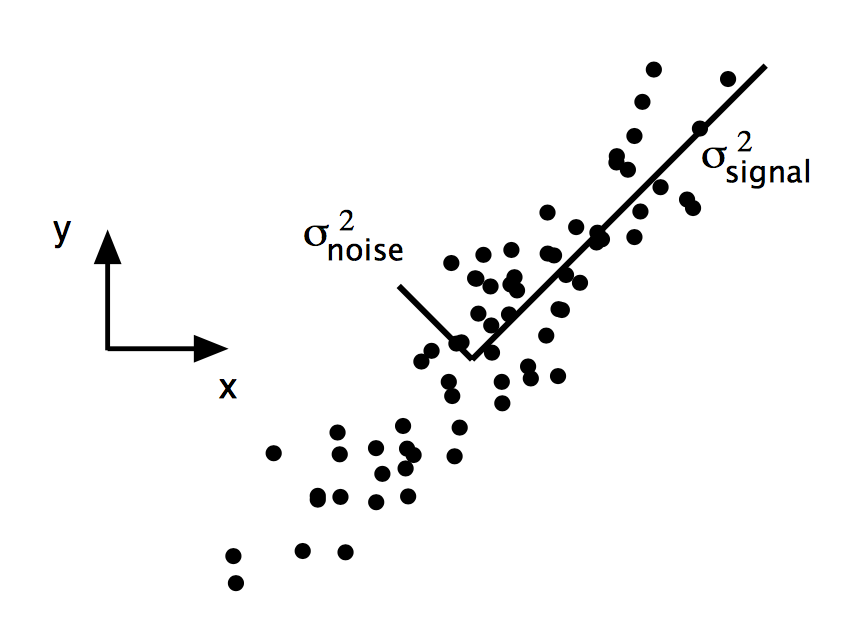
\includegraphics[scale=.6]{figures/fig2}}
\caption{A typical 2D example. The signal and noise variances $\sigma^2_{signal}$ and $\sigma^2_{noise}$ are graphically represented by the two lines subtending the cloud of data. The largest direction of variance lie along the best-fit line}
\label{fig2}
\end{figure}

 In a simple $2D$ example like in Figure \ref{fig2}, $\pmb{P}$ acts as a generalized rotation to align a basis with the axis of maximal variance. In multiple dimensions this could be performed by a simple algorithm:
 \begin{enumerate}
\item Select a normalized direction in m-dimensional space along which the variance in $\pmb{X}$ is maximized. Save this vector as $\pmb{p_1}$ .
\item Find another direction along which variance is maximized, however, because of the orthonormality condition, restrict the search to all directions orthogonal to all previous selected directions. Save this vector as $\pmb{p_2}$
\item Repeat this procedure until $D$ vectors are selected.
 \end{enumerate}
The resulting ordered set of $\pmb{p}$'s are the principal components.




\subsection{Solving PCA in EVD Approach}
We derive our first algebraic solution to PCA based on an important property of eigenvector decomposition. Once again, the data set is $\pmb{P}$, an $D \times N$ matrix, where $D$ is the number of measurement types and $N$ is the number of samples. The goal is summarized as follows

\begin{center}
\begin{tabular}{p{12cm}}
Find some orthonormal matrix $\pmb{P}$ in $\pmb{Y = PX}$ such that $\pmb{C_Y \equiv \dfrac{1}{N}XX}^T$ is a diagonal matrix. The rows of  $\pmb{P}$  are the principal components of  $\pmb{X}$ 
\end{tabular}
\end{center}
We begin by rewriting $\pmb{C_Y}$ in terms of the unknown variable

\begin{align*}
\pmb{C_Y} &= \dfrac{1}{N}\pmb{YY}^T\\
&= \dfrac{1}{N}\pmb{(PX)(PX)}^T\\
&= \dfrac{1}{N}\pmb{PXX}^T\pmb{P}^T\\
&= \pmb{P}(\dfrac{1}{N}\pmb{XX}^T)\pmb{P}^T\\
\pmb{C_Y} &= \pmb{PC_XP}^T 
\end{align*}

Note that we have identified the covariance matrix of $\pmb{X}$  in the last line.

Our plan is to recognize that any symmetric matrix A is diagonalized by an orthogonal matrix of its eigenvectors (by Theorems 3 and 4 from Appendix \ref{ch:linear}). For a symmetric matrix $\pmb{A}$  Theorem 4 provides $\pmb{A = EDE}^T$, where $\pmb{D}$  is a diagonal matrix and $\pmb{E}$  is a matrix of eigenvectors of $\pmb{A}$  arranged as columns.

Now we comes the trick. We select the matrix $\pmb{P}$  to be a matrix where each row $\pmb{p_i}$  is an eigenvector of $\dfrac{1}{N}\pmb{XX}^T$ . By this selection, $\pmb{P \equiv E}^T$ . With this relation and Theorem 1 of Appendix \ref{ch:linear} ($\pmb{P}^{-1} = \pmb{P}^T$) we can finish evaluating $\pmb{C_Y}$.

\begin{align*}
\pmb{C_Y} &= \pmb{PC_XP}^T\\
&= \pmb{P(E}^T\pmb{DE)P}^T\\
&= \pmb{P(P}^T\pmb{DP)P}^T\\
&= \pmb{(PP}^T)\pmb{D(PP)}^T\\
&= \pmb{(PP}^{-1})\pmb{D(PP)}^{-1}\\
\pmb{C_Y} &= \pmb{D}
\end{align*}

It is evident that the choice of $\pmb{P}$ diagonalizes $\pmb{C_Y}$. This was the goal for PCA. We can summarize the results of PCA in the matrices $\pmb{P}$ and $\pmb{C_Y}$.

\begin{itemize}
\item The principal components of $\pmb{C_Y}$ are the eigenvectors of $\pmb{C_X}$ = $\dfrac{1}{N}\pmb{XX}^T$
\item The $i^{th}$ diagonal value of $\pmb{C_Y}$ is the variance of $\pmb{X}$ along $\pmb{p_i}$
\end{itemize}

\section{Practical Approach of EVD}
In practice computing PCA of a data set $\pmb{X}$ is done in two steps:
\begin{enumerate}
\item subtracting off the mean of each measurement type 
\item computing the eigenvectors of $\pmb{C_X}$
\end{enumerate}
\section{Singular Value Decomposition (SVD)}
Let $\textbf{X}$ be an arbitrary $N \times D$ matrix and $\pmb{X}^T\pmb{X}$ be a rank $r$, square, symmetric $D \times D$ matrix. 

\subsection{Performing SVD}
To do Singular Value Decomposition of matrix \textbf{X} let us assume that:
\begin{itemize}
\item $\{\hat{v} _1,\hat{v} _2, \dots ,\hat{v} _r\}$ is the set of orthonormal $D \times 1$ eigenvectors with associated eigenvalues $\{\lambda _1, \lambda _2, \dots, \lambda _r\}$ for the symmetric matrix $\pmb{X^TX}$
$$(  \pmb{X^TX} ) \hat{v} _i = \lambda _i\hat{v} _i$$

\item
$\sigma_i \equiv \sqrt{\lambda_i}$ are positive real and termed the singular values.

\item 
$\{\hat{u} _1,\hat{u} _2, \dots ,\hat{u} _r\}$ is the set of $N \times 1$ vectors defined by $\pmb{\hat{u}_i \equiv \dfrac{1}{\sigma_i}X\hat{v}_i}$

\begin{equation}
\label{eq3}
\pmb{\sigma_i\hat{u}_i \equiv X\hat{v}_i}
\end{equation}

\end{itemize}

This result says a quite a bit. $\pmb{X}$ multiplied by an eigenvector of $\pmb{X^TX}$ is equal to a scalar times another vector. We can summarize this result for all vectors in one matrix multiplication by following the prescribed construction in Figure \ref{SVD}. We start by constructing a new diagonal matrix $\sum$.

$$\pmb{
\sum \equiv
\left[
    \begin{array}{cccccc}
    \sigma_1                                    \\
    & \ddots & & &\text{\huge0}\\
	& & \sigma_{\tilde{r}} \\
	& & &0 \\
	& \text{\huge0} &  & &\ddots             \\
      &               &   &   &  & 0
    \end{array}
    \right]
    }
$$

where $\sigma_{\tilde{1}} \geq \sigma_{\tilde{2}} \geq  \dots \geq \sigma_{\tilde{r}}$ are the rank-ordered set of singular values. Likewise we construct accompanying orthogonal matrices,
$$\pmb{V} = 
	\left[
	\begin{array}{cccc}
	\pmb{\hat{v}_{\tilde{1}}} &\pmb{\hat{v}_{\tilde{2}}} & \dots &\pmb{\hat{v}_{\tilde{D}}}
	\end{array}
	\right]
$$   
$$ \pmb{U} = 
	\left[
	\begin{array}{cccc}
	\pmb{\hat{u}_{\tilde{1}}} &\pmb{\hat{u}_{\tilde{2}}} & \dots &\pmb{\hat{u}_{\tilde{N}}}
	\end{array}
	\right]
$$   

where we have appended an additional ($D - r$) and ($N - $r) orthonormal vectors to ``fill up'' the matrices for \textbf{V} and \textbf{U} respectively (i.e. to deal with degeneracy issues).
 Figure \ref{SVD} provides a graphical representation of how all of the pieces fit together to form the matrix version of \textit{SVD}.
$$\pmb{XV = U\sum}$$
where each column of $\pmb{V}$ and $\pmb{U}$ perform the scalar version of the decomposition (Equation \ref{eq3}). Because $\pmb{V}$ is orthogonal, we can multiply both sides by $\pmb{V^1}$ = $\pmb{V}^T$ to arrive at the final form of the decomposition.
\begin{equation}
\label{eq4}
\pmb{X = U \sum V}^T 
\end{equation}
Although derived without motivation, this decomposition is quite powerful. Equation \ref{eq4} states that any arbitrary matrix \textbf{X} can be converted to an orthogonal matrix, a diagonal matrix and another orthogonal matrix (or a rotation, a stretch and a second rotation)


\begin{figure}
\centering
\frame{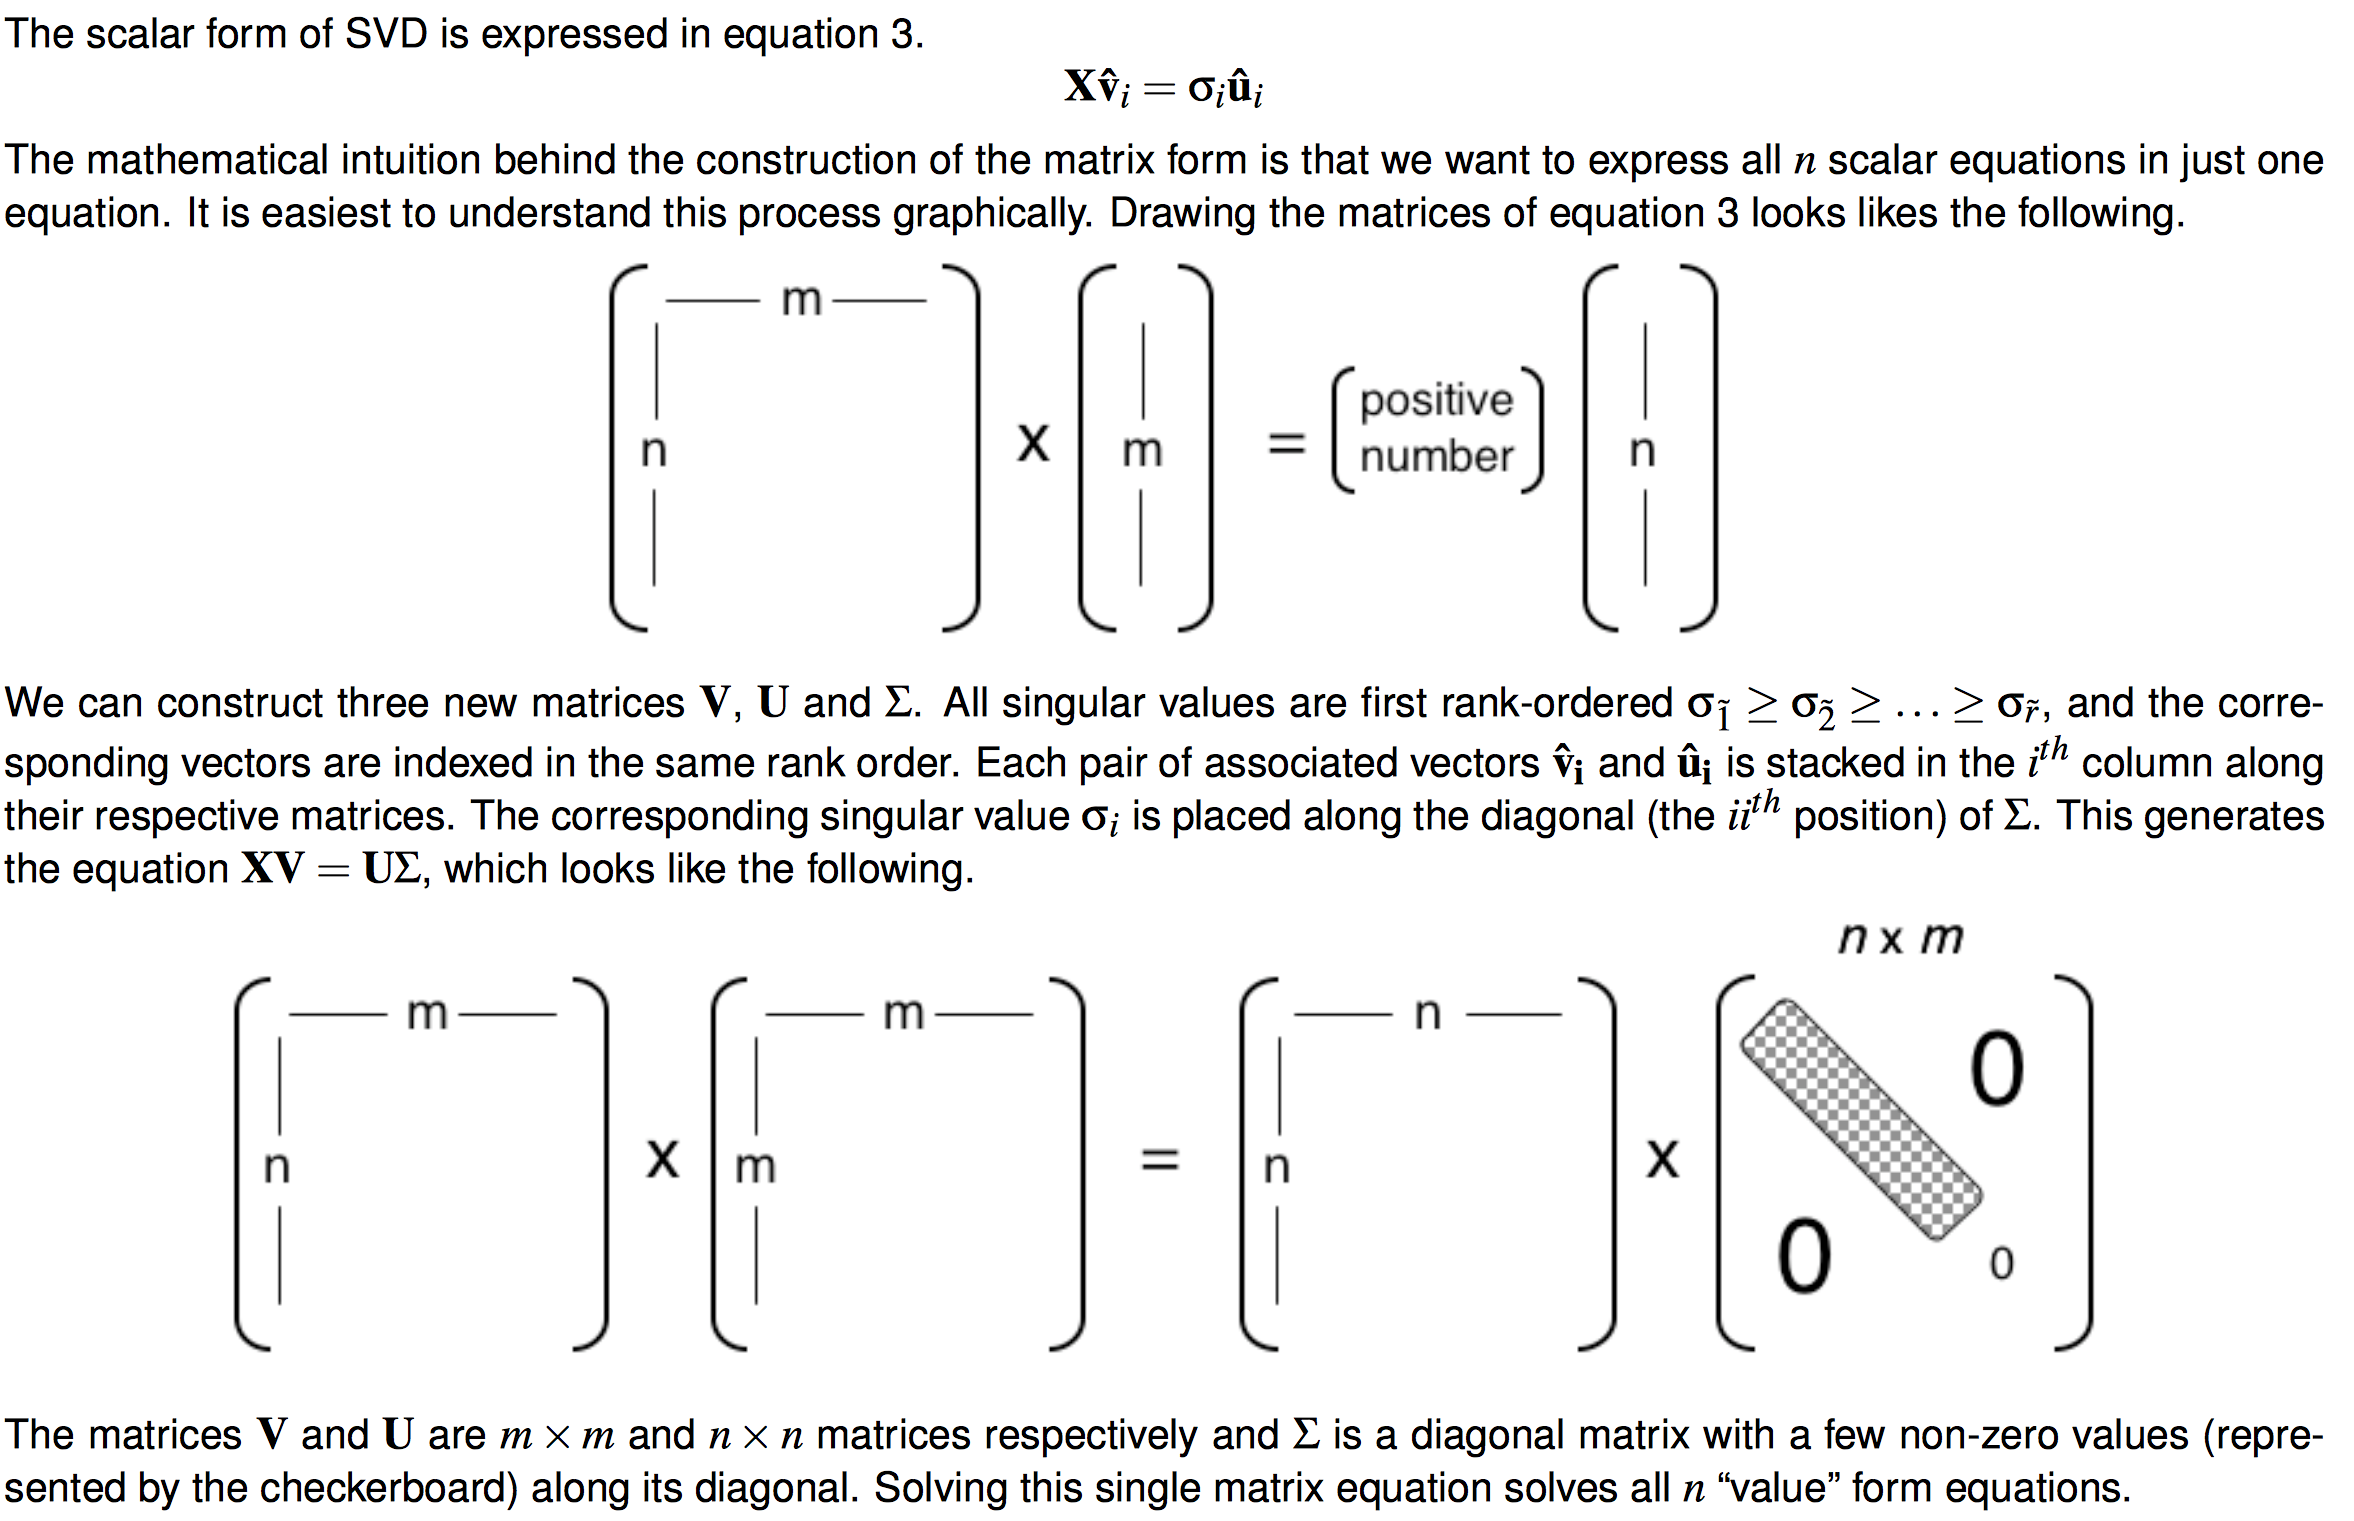
\includegraphics[scale=.38]{figures/SVD}}
\caption{Construction of the matrix form of SVD \ref{eq4} from the scalar form \ref{eq3}}
\label{SVD}
\end{figure}

\subsection{Linking SVD with EVD}

How does this link in to the previous \textit{EVD} analysis of PCA? Let us consider the $N \times D$ matrix, \textbf{X}, for which we have a singular value decomposition, $\pmb{X = U \sum V}^T$. There is a theorem from linear algebra which says that the non-zero singular values of \textbf{X} are the square roots of the nonzero eigenvalues of $\pmb{AA}^T$ or $\pmb{A}^T\pmb{A}$. 

\newpage The former assertion for the case $\pmb{A}^T\pmb{A}$ is proven in the following way:
\begin{align*}
\pmb{A}^T\pmb{A}  &= (\pmb{U\sum V}^T)^T(\pmb{U\sum V}^T)\\
										   &= (\pmb{V\sum}^T\pmb{U}^T)(\pmb{U\sum V}^T)\\
										   &= \pmb{V}(\sum^T\sum)\pmb{V}^T
\end{align*}

We observe that $\pmb{A}^T\pmb{A}$ is similar to $\sum^T\sum$ and thus it has the same eigenvalues. Since $\sum^T\sum$ is a square ($D \times D$), diagonal matrix, the eigenvalues are in fact the diagonal entries, which are the squares of the singular values. Note that the non-zero eigenvalues of each of the covariance matrices, $\pmb{AA}^T$ and $\pmb{A}^T\pmb{A}$ are actually identical.


It should also be noted that we have effectively performed an eigenvalue decomposition for the matrix, $\pmb{A}^T\pmb{A}$. Indeed, since AT A is symmetric, this is an orthogonal diagonalisation and thus the eigenvectors of $\pmb{A}^T\pmb{A}$ are the columns of $\pmb{V}$. This will be important in making the practical connection between the SVD and and the PCA of matrix X, which is what we will do next.


Returning to the original $N \times D$ data matrix, $\pmb{X}$, let us define a new $D \times N$ matrix, $\pmb{Z}$:

$$\pmb{Z} = \dfrac{1}{\sqrt{N-1}}\pmb{X}^T$$

Recall that since the m rows of $\pmb{X}$ contained the $N$ data samples, we subtracted the row average from each entry to ensure zero mean across the rows. Thus, the new matrix, $\pmb{Z}$ has columns with zero mean. Consider forming the $D \times D$ matrix, $\pmb{Z}^T\pmb{Z}$:
\begin{align*}
\pmb{Z}^T\pmb{Z} &= (\dfrac{1}{\sqrt{N-1}}\pmb{X}^T)^T(\dfrac{1}{\sqrt{N-1}}\pmb{X}^T)\\
&= \dfrac{1}{N-1}\pmb{XX}^T\\
i.e. \  \pmb{Z}^T\pmb{Z} &= \pmb{C_x}
\end{align*}
We find that defining $\pmb{Z}$ in this way ensures that $\pmb{Z}^T\pmb{Z}$ is equal to the covariance matrix of $\pmb{Z}$, $\pmb{C_x}$. From the discussion in the previous section, the principal components of $\pmb{X}$ (which is what we are trying to identify) are the eigenvectors of $\pmb{C_x}$. Therefore, if we perform a singular value decomposition of the matrix $\pmb{Z}^T\pmb{Z}$, the principal components will be the columns of the orthogonal matrix, $\pmb{V}$.

The last step is to relate the \textit{SVD} of $\pmb{Z}^T\pmb{Z}$ back to the change of basis:

$$\pmb{Y} = \pmb{PX}$$

We wish to project the original data onto the directions described by the principal components. Since we have the relation $\pmb{V} = \pmb{P}^T$ , this is simply: 

$$\pmb{Y} = \pmb{V}^T\pmb{X}$$

If we wish to recover the original data, we simply compute (using orthogonality of $\pmb{V}$): 

$$\pmb{X} = \pmb{VY}$$

\subsection{SVD for Dense Matrices}


Golub and Kahan \cite{golub} introduced a two-step approach for computing SVD: convert the input matrix to a bidiagonal one and then perform SVD on the bidiagonal matrix. Demmel and Kahan \cite{demmel} improved this approach by adding another step before bidiagonalization, which is QR decomposition. \cite{elgamal} refered to this method as SVD-Bidiag, which has the following three steps for a given matrix $\pmb{Y}$:
\begin{enumerate}
\item
compute the QR decomposition of $\pmb{Y}$, which results in an orthogonal matrix \textbf{Q} and an upper triangular matrix $\pmb{R}$ 

\item
transform \textbf{R} to a bidiagonal matrix $\pmb{B}$
\item 
compute SVD on $\pmb{B}$
\end{enumerate}
The SVD-Bidiag algorithm is implemented in \textit{RScaLAPACK}. Their analysis showed that the computational complexity of the SVD-Bidiag algorithm is dominated by the QR decomposition and bi-diagonalization steps, and is given by $\mathcal{O}(ND^2 + D^3)$. Therefore, the SVD-Bidiag algorithm is only suitable when D is small. More details can be found in \cite{elgamal}.

\subsection{SVD for Sparse Matrices}
SVD can be computed efficiently for sparse matrices using Lanczos' algorithm \cite{roman}, which has a computational complexity of $\mathcal{O}(Nz^2)$, where $z$ is the number of non-zero dimensions (out of \textbf{D} dimensions). More details can be found in \cite{elgamal}.


\section{Stochastic SVD (SSVD)}
Randomized sampling techniques have recently gained popularity in solving large-scale linear algebra problems. The work in \cite{halko} describes a randomized method to compute approximate decomposition of matrices, which is referred to as stochastic SVD (SSVD). SSVD has two steps: 
\begin{enumerate}
\item It uses randomized techniques to compute a low-dimensional approximation of the input matrix
\item It performs SVD on the approximation matrix
\end{enumerate}
The accuracy of the results depends on the performance of the randomized techniques and the size of the approximation matrix. Accuracy can be improved through running the randomization step multiple times. Therefore, SSVD has the flexibility of trading off the accuracy of the results with the required computational resources.

\section{Computational Complexity}
Computational complexity of SSVD is dominated by the first step, which is $\mathcal{O}(DNd)$. This is a much better complexity than the previous techniques, because $d$ is typically much smaller than $D$ and is usually a constant. However, SSVD requires exchanging multiple intermediate matrices, which may cause a problem for scalability. The amount of intermediate data can be up to $\mathcal{O}(max(Nd,d2))$ \cite{elgamal}.
\section{Probabilistic PCA (PPCA)}
We will be trying to present \textit{PPCA} in some kind of detail. For this we will follow the research work of Tipping and Bishop \cite{bishop}
\subsection{What is PPCA}
We can obtain a probabilistic formulation of PCA by introducing a Gaussian latent i.e. unobserved variable model. This kind of model is highly related to statistical factor analysis. First let us define some quantity:
\begin{itemize}
\item $\pmb{y}$ is a $D$ dimensional observed data vector
\item $\pmb{x}$ is a $d$ dimensional latent variable
\item $\pmb{W}$ is a $D \times d$ transformation matrix
\item the columns of $\pmb{W}$ are the principal components
\item $\pmb{\mu}$ is the dimension wise mean vector of $\pmb{y}$. This parameter allows the data to have non zero mean
\item $\pmb{\epsilon}$ is a $D$-dimensional zero-mean  noise variable
\item Here $\pmb{x}$, $\pmb{\epsilon}$, $\pmb{y}$ are normal distributed i.e. Gaussian distributed
\begin{align*}
\pmb{x} &\sim \mathcal{N}(\pmb{0},\pmb{I})\\
\pmb{\epsilon} &\sim \mathcal{N}(\pmb{0},\pmb{\sigma^2I})\\
\pmb{y} &\sim \mathcal{N}(\pmb{\mu},\pmb{WW}^T+\pmb{\sigma^2})
\end{align*}
where $\pmb{x} \sim \mathcal{N}(\pmb{u},\sum)$ denotes the Normal distribution with $\pmb{u}$ mean and $\sum$ covariance matrix.
\end{itemize}
A latent variable model seeks to relate a $D$-dimensional observation vector $\pmb{y}$ to a corresponding $d$-dimensional vector of latent variables $\pmb{x}$ where the relationship is linear:
\begin{equation}
\pmb{y} = \pmb{Wx}+ \pmb{\mu} + \pmb{\epsilon}
\label{PPCA:eq1}
\end{equation}
The motivation is that, with $d < D $, the latent variables will offer a more parsimonious explanation of the dependencies between the observations. The model parameters may thus be determined by maximum-likelihood, As there is no closed-form analytic solution for finding $\pmb{W}$ and $\pmb{\sigma}^2$, their values must be obtained via an iterative procedure.

\subsection{The Probability Model}
The use of the isotropic Gaussian noise model $\mathcal{N}(\pmb{0},\pmb{\sigma^2I})$ for   in conjunction with equation (\ref{PPCA:eq1}) implies that the $\pmb{x}$-conditional probability distribution over $\pmb{y}$-space is given by:
\begin{equation}
\label{PPCA:eq2}
\pmb{y|x} \sim \mathcal{N}(\pmb{Wx}+\pmb{\mu}, \pmb{\sigma}^2\pmb{I})
\end{equation}
With the marginal distribution over the latent variables also Gaussian and conventionally defined by $\pmb{x} \sim \mathcal{N}(\pmb{0},\pmb{I})$, the marginal distribution for the observed data $\pmb{y}$ is readily obtained by integrating out the latent variables and is likewise Gaussian:
\begin{equation}
\label{PPCA:eq3}
\pmb{y} \sim \mathcal{N}(\pmb{\mu},\pmb{C})
\end{equation}
where the observation covariance model is specified by $\pmb{C}=\pmb{WW}^T+\pmb{\sigma^2}$. given $N$ observations $\{\pmb{y_n}\}^N_1$ as the input data, the log likelihood of data is given by:
\begin{align}
\label{PPCA:eq4}
{\mathcal{L}(\{ \pmb{y_r}\}^N_1)} &= \sum_{n=1}^N \ln{p(\pmb{n_r})} \nonumber \\
&= -\dfrac{1}{N}\{D*\ln(2\pi) + \ln|\pmb{C}| + tr(\pmb{C}^{-1}*\pmb{S})\}
\end{align}
where $\pmb{S}$ is the sample covariance matrix of data $\pmb{\{y_r\}}$ given by:
\begin{equation}
\label{PPCA:eq5}
\pmb{S} = \dfrac{1}{N} \sum_{n=1}^N (\pmb{y_r - \mu})(\pmb{y_r - \mu})^T
\end{equation}
and $tr(\pmb{M})$ is the trace of matrix $\pmb{M}$

\subsection{Properties of the Maximum-Likelihood Estimators}
According to \cite{bishop}, the likelihood equation \ref{PPCA:eq4} is maximized when:
\begin{equation}
\label{PPCA:eq7}
\pmb{W}_{ML} = \pmb{U}_d \sqrt{\pmb{\Lambda}_d - \sigma^2\pmb{I}}\pmb{R}
\end{equation}
where:

where the $d$ column vectors in the $D \times d$ matrix $\pmb{U}_d$ are the principal eigenvectors of $\pmb{S}_d$, with corresponding eigenvalues $\{\lambda_1, \dots , \lambda_d\}$ in the $d \times d$ diagonal matrix $\pmb{\Lambda}_d$, and $\pmb{R}$ is an arbitrary $d \times d$ orthogonal rotation matrix. Thus, from Equation (\ref{PPCA:eq7}), the latent variable model defined by Equation (\ref{PPCA:eq1}) effects a mapping from the latent space into the principal subspace of the observed data.

It may also be shown that for $\pmb{W} = \pmb{W}_{ML}$, the maximum-likelihood estimator for $\sigma^2$ is given by:
\begin{equation}
\label{PPCA:eq8}
\sigma^2_{ML} = \dfrac{1}{D - d} \sum_{i=d+1}^D \lambda_i
\end{equation}
which has a clear interpretation as the variance `lost' in the projection, averaged over the lost dimensions.
\subsection{An EM Algorithm for Probabilistic PCA}
In the EM approach to maximising the likelihood for PPCA, we consider the latent variables  $\{\pmb{x}_n\}$ to be `missing' data and the `complete' data to comprise the observations together with these latent variables. The corresponding complete-data log-likelihood is then:

\begin{equation}
\label{PPCA:eq22}
\mathcal{L}_C = \sum^N_{n=1} \ln {p(\pmb{y}_n),\pmb{x}_n)} 
\end{equation}

The corresponding E-step and M-step are given below:
\begin{align}
\label{PPCA:EM}
\text{\textbf{E-step:}} \ \ \ \ \ \ \ \  \langle \pmb{x}_n \rangle &= \pmb{M}^{-1}\pmb{W}^T(\pmb{y}_{n} - \pmb{\mu}) \\
\label{PPCA:EM1}
\text{\textbf{E-step:}}  \ \ \ \ \langle \pmb{x}_n\pmb{x}_n^T \rangle &= \mathlarger{\sigma}^2\pmb{M}^{-1}+ \langle \pmb{x}_n\rangle \langle\pmb{x}_n \rangle ^T\\
\label{PPCA:EM2}
\text{\textbf{M-step:}} \ \ \ \ \ \ \ \ \ \ \  \pmb{\Tilde{W}} &= \left[ \mathlarger{\sum}_{n=1}^N(\pmb{y}_n - \pmb{\mu)} \langle \pmb{x}_n \rangle^T  \right] \left[ {\mathlarger{\sum}_{n=1}^N}\langle \pmb{x}_n\pmb{x}_n^T \rangle \right]^{-1} \\
\label{PPCA:EM3}
\text{\textbf{M-step:}}  \ \ \  \ \ \ \  \ \ \ \ \mathlarger{\sigma}^2 &= \dfrac{1}{ND} \mathlarger{\sum}^N_{n=1} \left[    || \pmb{y}_n - \pmb{\mu} ||^2 - 2\langle \pmb{x}_n \rangle \widetilde{\pmb{W}}(\pmb{y}_n - \pmb{\mu}) + tr \left( \langle \pmb{x}_n\pmb{x}_n^T \rangle \widetilde{\pmb{W}}^T\widetilde{\pmb{W}}  \right) \right]
\end{align}

In order to make the EM algorithm look simple we define:
\begin{align*}
\pmb{E}_n &= \langle \pmb{x}_n \rangle\\
\pmb{F}_n &= \langle \pmb{x}_n\pmb{x}_n^T \rangle\\
\pmb{Y}_m &= (\pmb{y}_n - \pmb{\mu})\\
{Frob(\pmb{Y}_m)} &= || \pmb{y}_n - \pmb{\mu} ||^2
\end{align*}
Therefore, we can write the EM steps with simplified notations:
\begin{align*}
\text{\textbf{E-step:}} \ \ \ \ \  \pmb{E} &= \pmb{M}^{-1}\pmb{W}^T(\pmb{Y}_{m}) \\
\text{\textbf{E-step:}} \ \ \ \ \  \pmb{F} &= \mathlarger{\sigma}^2\pmb{M}^{-1}+ \pmb{E}\pmb{E}^T\\
\text{\textbf{M-step:}} \ \ \ \  \pmb{\widetilde{W}} &= (\pmb{Y}_m\pmb{E}^T)\pmb{F}^{-1} \\
\text{\textbf{M-step:}} \ \ \ \ \mathlarger{\sigma}^2 &= \dfrac{1}{ND} \left[    Frob(\pmb{Y}_m) - 2 \mathlarger{\sum}^N_{n=1} \pmb{E}_n^T \widetilde{\pmb{W}}{\pmb{Y}_m}_n + tr \left(\pmb{F} \widetilde{\pmb{W}}^T\widetilde{\pmb{W}}  \right) \right]
\end{align*}

Iterating Equation (\ref{PPCA:EM}), (\ref{PPCA:EM1}), (\ref{PPCA:EM2}), (\ref{PPCA:EM3}) upto convergence, we can make a good approximation of both $\pmb{W}$ and $\pmb{\mathlarger{\sigma}^2}$.
The basic algorithm of PPCA is given below:

\begin{algorithm}[!htbp]
\caption{Basic PPCA}
\begin{algorithmic}[1]
	\STATE $W = normrnd(D,d)$
	\STATE $ss=normrnd(1,1)$
	\STATE $Y_m=columnMean(Y)$
	\STATE  $Y_c=Y-Ym$
	\WHILE {$(!Stop\_Condition)$}
		\STATE $M = W^T * W + ss * I$
		\STATE $X = Y_c * W * M^{-1}$
		\STATE $XtX = X^T * X + ss * M^{-1}$
		\S	TATE $YtX = Y_c^T * X$
		\STATE $W = YtX \times$ \textit{invert($XtX$)}
		\STATE $ss2 = trace(XtX * W^T * W)$
		\STATE $ss3= \sum_{n=1}^N X_n * W^T * {Y_c}_n$
		\STATE $ss = (||Y c||^2_F + ss2-2 * ss3)\times N^{-1} \times D^{-1}$
	\ENDWHILE
\label{basic}
\end{algorithmic}
\end{algorithm}

 
\section{Recent Implementation of \textit{sPCA}}
\cite{elgamal} presented a  scalable implementation of Probabilistic PCA for distributed platforms such as MapReduce and Spark. 
\subsection{Special Features}
The implementation of \textit{sPCA} has a good number of features:
\subsubsection{Mean Propagation to Leverage Sparsity}
The first optimization they propose is the mean propagation idea, which preserves and utilizes the sparsity of the input matrix $\pmb{Y}$. PPCA requires the input matrix to be mean-centered, meaning that the mean vector $\pmb{\mu}$ must be subtracted from each row of the original matrix $\pmb{Y}$. Large matrices, however, are mostly sparse, with many zero elements. Sparse matrices can achieve a small disk and memory footprint by storing only non-zero elements, and performing operations only over non-zero elements. Subtracting the non-zero mean from the matrix would make many elements non-zero, so the advantage of sparsity is lost.

To avoid the problems of subtracting the mean, they keep the original matrix $\pmb{Y}$ and the mean $\pmb{\mu}$ in two separate data structures. they did not subtract the mean $\pmb{\mu}$ from $\pmb{Y}$. Rather, they propagate the mean throughout the different matrix operations.
\subsubsection{Minimizing Intermediate Data}
Intermediate data can slow down the distributed execution of any PCA algorithm, because it needs to be transferred to other nodes for processing to continue. Their second optimization is job consolidation, which means merging multiple distributed jobs into one in order to reduce the communication between these jobs.
\subsubsection{Efficient Matrix Multiplication}
PPCA requires many matrix multiplications, which are expensive operations in a distributed setting. To appreciate the techniques that \textit{sPCA} employs to overcome the inefficiency of matrix multiplication, they briefly explain different possible implementations of this operation.
\subsubsection{Efficient Frobenius Norm Computation}
The PPCA algorithm requires computing the Frobenius norm of the mean-centered input matrix. To solve this problem, they design an algorithm which does not even require creating the dense vector. Many machine learning algorithms compute various norms of matrices. The proposed method for optimizing the computation of the Frobenius norm can be extended to other matrix norms using similar ideas. Thus, this simple optimization can benefit several other machine learning algorithms.

\subsection{Limitations}
Despite of having some wonderful features \textit{sPCA} has some limitations also. We can discuss these limitations from two aspects.

\begin{enumerate}
\item The approach is not applicable for high dimensional data or we can say tall and wide big data. Though the approach has done some efficient use of memory by reducing the generation of intermediate data, it still runs out of memory while running on big data whose vertical dimension is in the range of millions. We failed to run \textit{sPCA} on dataset of dimension $10M\times5M$ in our set-up cluster where we have machines with $64GB$ of RAM.\\   

\item There was no implementation on geographically distributed big data. In current world where data is distributed across national border to ensure fast access and national data sovereignty, it is necessary to be capable of doing data analysis on such geo-distributed data. However, \textit{sPCA} did not indicate a process of generating some kind of partial result and later accumulate them to produce the final analytical results.
\end{enumerate}




%In this paper, we explore these two issues in depth. We will propose a solution which is capable of handling \textit{Tall and Wide} big data and at the same time can perform on geographically distributed datasets where there is no provision of passing raw data across the data center. 


%The rest of this paper is organized as follows. In Section II, we discuss the background of PPCA showing its valuable advantages as well as some limitations. In Section III, we analyse already established approach \textit{sPCA}. We present our proposed implementation of PPCA on geographically distributed \textit{Tall and Wide} big data in Section IV. We justify our contribution in Section V. Section VI presents some of the properties of our approach and Section VII presents our experimental evaluation. Finally, Section VIII concludes the paper.

\endinput

% Citation examples

%Chapter-4 Our Focus

\chapter{Our Focus}
	\label{c:4}
In current world, the rate of generation of data is quite large. We live in an age of Big Data and Internet of Things (loT). The term Big Data is not really an overstatement. Numerous web services share and collect data of huge scale, typically in terabytes range, and the data includes various aspects of users, for example, clicks, visits, likes, shares, comments, reviews, ratings, tweets, photos, videos etc. Apart from these web services, big data is also generated by countless sensors all around the globe to gather valuable information about respective fields. For example, closed circuit cameras recording is a good source of big data. In a nutshell, every electronic device, Internet services, embedded system and sensor the globe produce and transmit data and big data is being generated by these multiple sources at an alarming velocity, volume and variety.

For researchers, however, big data brings new sets of challenges like how to efficiently and
effectively handle big data in commodity computers, how to apply conventional algorithms, how
to properly manage big data in distributed setting etc. Specially, in field of machine leaning and
Pattern recognition, big data poses a threat, because the conventional algorithms were designed
solely to fulfil its purpose where entire dataset can fit in memory. Distributed setting was not
taken into consideration. In nutshell, to extract any meaningful insight from this big data, we
need powerful tools to analyse it, elastic frameworks to cope up with its sheer volume and most
importantly we have to rethink and redesign existing algorithms which are most suitable for
smaller sized dataset and do not take advantage of clusters.

In this chapter we will discuss the present issues that we are going to take into consideration in our research. We will indicate the challenges we targeted and in later chapters we will give our proposals in order to minimize these challenges in data analysis.
\section{Tall and Wide Data}
In general, the width of data means the number of features that each data sample is comprised of. In present world, this features count is increasing at large scale. The feature count or width of data sample can also be named as ``Dimension of Data". One of the most effective use of PCA is dimensionality reduction. Many machine learning algorithms are not capable of handling data with large dimension. Therefore, we can use PCA to reduce the width of data then fit them in some kind of machine learning model. This present some kind of new challenge. The present PCA algorithms are not that much capable of handle very wide data that is tall also. Therefore before making the data suitable for machine learning models by dimensionality reduction, the PPCA algorithm has to deal with the curse of tall and wide data. The present implementation of \textit{sPCA} done good number of optimization to make efficient use of memory. Still it is not capable of handling tall and wide data. The memory overflow occurs while computing the intermediate results. 
\section{The Blessings and Curses of Geo Distributed Data}
Geo Distributed Data has both positive and negative sides. In this section we will show some of them.
\subsection{The Bright Sides}
\subsubsection{Assurance of Faster Data Access}
As data stays closer to end users, the users can easily access the data with lower latency.
\subsubsection{Protection of National Privacy}
Now data contains some kind national privacy. Moreover no nation will want the data of its people to cross the national boundary. As a result there are regulations on na
\subsubsection{Sparsity of Data Centers}
The Data centers are not places on the same regions. Multiple Data centers are placed in different place. 
\subsubsection{Development in Business Sector}
As different giant companies establishing there data center in different countries, so the business is growing.


\subsection{The Dark Sides}
\begin{itemize}
	\item New Challenges in Data Analysis
	\item Unavailability of Global View 
	\item Break Down of Data Consistency
\end{itemize}


\chapter{Preliminary Work on Regression Analysis}
	\label{c:5}
The field of geo-distributed data analysis is quite vast. A detailed study of these aspects of the distributed approach of data analysis is beyond the scope of our tasks during the first few days. As a part of learning how to work on data analytic what we wanted to introduce is a problem specific approach. We were interested in doing ``Regression Analysis" on data located at different geographical areas all around the world. Primarily we have worked out with only two variants of regression analysis ``Linear Regression" and ``Polynomial Regression". So we can say the other variants as well as other problem oriented approaches were not be covered in this chapter. 

\section{Contribution}
Summarizing, our main contributions are:
\begin{itemize}
\item We propose an approach of regression analysis that is deals with geo-distributed data and provide an in-depth study of the relative merits against centralized approach.
\item We propose a system that builds upon Apache Hadoop MapReduce \cite{116} framework and extends their functionality to support multi data center learning applications.
\item We propose an approach that will minimize the number of transfers among data centers thus minimize the inter data center bandwidth utilization.
\item We propose an approach that is a combination of the two concepts \emph{Data Parallelism} \cite{117} and \emph{Model Parallelism} \cite{117}.
\item We present experimental results implemented on \emph{Amazon Web Services (AWS)}. 
\end{itemize}

\section{Problem Specification}
We were interested in building a regression model on geographically distributed data. We had the intention of using least square regression analysis. In order to facilitate the study, we formalize the problem in two dimensions: 
\begin{enumerate}
\item We will make our assumptions about the data, its type, size and distribution.
\item We limit the regression analysis to 2nd order only. That means we would try only ``Linear Regression" and ``Polynomial Regression".
\end{enumerate}
So we can see that regression analysis on higher order and other classes of regressions (eg. ``Logistic Regression") will not be covered in this paper.

\subsection{Assumptions on Data}
To keep the analysis simple we used data only in text format. There may be multiple text files which will be considered as input files to our program. every text file contains multiple lines and each of these lines will be tokenized and the information will be extracted.

\subsection{Distribution of Data}
In order to run our program on distributed data we used cloud computing facilities of \emph{Amazon Web Services (AWS)}. We created two different data centers in two different geographic location, ``North Virginia" and ``Malaysia". Every data center was consisted of two \emph{Linux} instances. Among the two instances  of a data center we named one of  them as \emph{NameNode} and other one as \emph{DataNode}. The \emph{NameNode} works as a master node of its corresponding data center. Full data of a particular data center is further distributed in its \emph{NameNode} and \emph{DataNode}. Any kind of jobs on the the data of a data center can also be split and distributed among its instances. 


\section{Approach}
We created \emph{Hadoop MapReduce} cluster on \emph{Amazon AWS}. Our implementation needs to obtain resources like CPU cores, Memory during the partial computation on data in a particular data center in a uniform basis. Such resources are managed by a resource manager in the \emph{Hadoop} cluster system. Further, \emph{Apache Hadoop YARN}'s new federation feature allows us to view multiple data centers as a single one.
Data on a data center is organized by \emph{Haddop} File System \emph{HDFS}. 

\subsection{Learning Process}
For running our regression computation on geographically distributed data we mainly focused on two concepts:
\begin{itemize}
\item \textbf{Data Parallelism} It is the main idea of distributed data. Its can be seen as application of a single instruction to multiple data items. It focuses on distributing the data across different nodes, which operate on the data in parallel. As an example we can mention the array operations. In case of summing the data of an array, we can make multiple partition of the array and then apply summation formula on each partition. The aggregated result will give us the final summation. In our distributed data organization, data are located in different location while we need to make the same computation on them. This can be achieved by making partial computation on each data partition and aggregate them at the end.   

\item \textbf{Model Parallelism} In case of model parallelism the system gives every processor the same data but applies a different model to it. Model parallelism finds its applications in deep learning. As we can see that data centers are generally composed of multiple machines, we can use that resource to speed up the computation. If any learning process consists of multiple types of computation then we can create different model and place them in different machines. Therefore, at the time of making partial learning from any data center, each machine can do its model task on a parallel basis and the whole result can be obtained at a lower time period.
\end{itemize}

The first innovation in our approach is that we intend to make a mixed use of both \emph{Data Parallelism} and \emph{Model Parallelism}. 
\begin{itemize}
\item Data that are distributed in different data centers located at different geographic location resemble the \emph{Data Parallelism} concept. 
\item Then in case of a single data center, every machines of that data center has a shared view on the data because of the \emph{HDFS} file system. In order to compute $n$ parameters, if the data center has $n$ machines then we can distribute the different computation in different machines. That means every machine will work on separate models in parallel. This gives the use of model parallelism. 
\end{itemize}


The parameter to passed among the data centers can be determined from the equations or regression. For example of we consider regression of second degree, it can be expressed as:
\begin{align*}
y &= y_{model} + \epsilon\\
y_{model} &= ax^2 + bx + c
\end{align*}
where,
\begin{align*}
y &= original\ value\\
y_{model} &= model\ value\\
\epsilon &= error\\
\epsilon &= y - y_{model}\\
\end{align*}




If we intend to use least square regression model then we have to minimize the total squared error


\begin{align*}
S &= \sum \epsilon ^ 2\\
&= \sum (y-y_{model})^2
\end{align*}

In the process of minimizing $S$ we get the necessary equation to find the co-efficients in matrix form:

\[
\left[
\begin{array}{ccc}
\sum x_i^4 &\sum x_i^3 &\sum x_i^2 \\
\sum x_i^3 &\sum x_i^2 &\sum x_i \\
\sum x_i^2 &\sum x_i &n
\end{array}
\right]
\left[
\begin{array}{c}
a\\b\\c
\end{array}
\right]
=
\left[
\begin{array}{c}
\sum x_i^2y\\\sum x_iy_i\\\sum y_i
\end{array}
\right]
\]

Here we have to compute 7 parameters that appear in the matrix form. Every data center will compute these parameters on its own data. Then they will be sent to the initiating data center. At the initiating data center all the parameter will be merged to get the final model.

\subsection{Algorithm}
The whole process is divided into two parts. First of all, every data center will compute parameters by executing computation on their corresponding partial data. This task will be handled by the child processes. And the initiating data center i.e. master data center will run the parent process. which will receive the partial computational result and merge them to built a complete regression model.

\begin{algorithm}[!htbp]
	\caption{Geo-Distributed Regression Analysis}
	 \label{algo:1}
	\begin{algorithmic} [1]
	\STATE \textbf{Input: }Data located at different geographic location
	\STATE \textbf{Output: }Regression model
	\STATE \underline{Parent Process}
	\STATE select an arbitrary data center as the initiating one, \emph{root}
	\WHILE{end of ``node list'' has not encountered}
		\STATE pick a data center, \emph{node}
		\STATE create a parallel executable child process with the parameters \emph{root} and \emph{node}
	\ENDWHILE
	\STATE $available = false$
	\WHILE{$available = false$}
		\IF{every partial computational files from every data centers are available}
			\STATE $available = true$
		\ENDIF
	\ENDWHILE
	\STATE merge all the partial computational files into a single one
	\STATE create final regression model using the merged files
	\end{algorithmic}
\end{algorithm}



\begin{algorithm}[!htbp]
    \caption{Geo-Distributed Regression Analysis}
	\begin{algorithmic} [1]
	\label{algo:2}
	\STATE \textbf{Input: }{Data located in corresponding local machines}
	\STATE \textbf{Input: }{Information of 2 nodes}
    \STATE \textbf{Output: }{Partial Parameter}
	\STATE \underline{Child Process}
	\STATE set the input and output locations of \emph{Hadoop} File System
	\STATE run the “Partial Regression Computation” program
	\IF{root and node are the same}
	
		\STATE the $node$ is the initiating data center $root$ itself
		\STATE rename the output files with information of $root$
		\STATE move the renamed files in the $Common Container$ location of $root$
	
	
	\ELSE
	
		\STATE the $node$ is a non initiating data center
		\STATE rename the output files with information of $node$
		\STATE send the renamed files in the $Common Container$ location of $root$
	
	\ENDIF
	\end{algorithmic}
\end{algorithm}


\newpage

From the algorithm, we can see that there will be two types of communication during the learning task:
\begin{itemize}
\item \textbf{Global Communication}
Every data center has multiple instances of machines. Among them only one will communicate with other data centers. Such machine will be considered as a master node. There will be message passing among the master nodes of data centers. Whenever a learning process is to be initialized one of the master nodes will issue command to each master nodes to start their partial computation. Again after the partial computation of each data centers the parameters will be passed towards the initializing data center's master node. In this way the master nodes of every data center will create a Global Communication Group among them.
\item \textbf{Local Communication}
Whenever a data center's master node receives the command of partial computation, it will communicate with its other machines i.e. slave nodes. The computation task will be distributed among all the machines of that data center in order to exploit the advantage of \emph{Model Parallelism}. We can say that each machine of a data center will work on one or some specific job. At the completion of each job each separate machine will write its result in a common container of the master node from where all the partial results will be transferred to initialing data center's master node.
\end{itemize}
The communication group are shown in Figure \ref{communication}


\begin{figure}[!htbp]
\centering
\frame{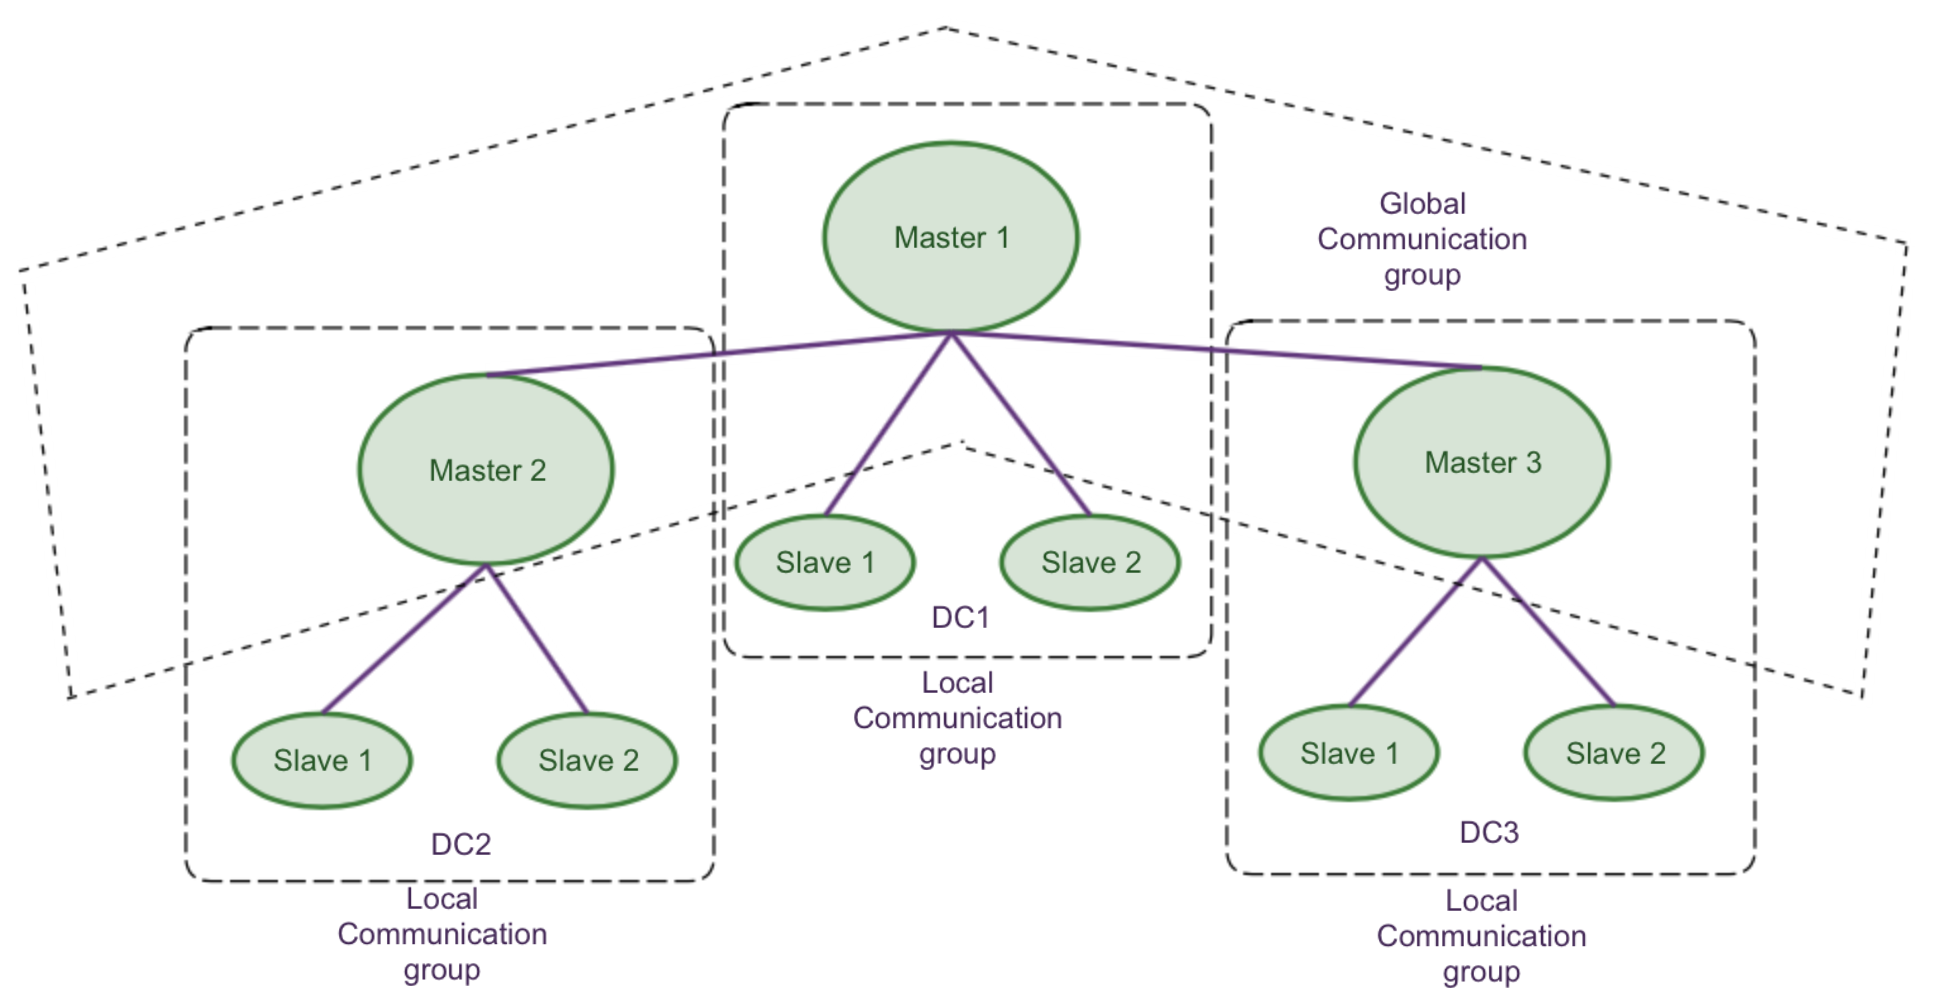
\includegraphics[width=5.2in]{communication.png}}
\caption{Communication Groups}
\label{communication}
\end{figure}


Figure \ref{learning} shows how the algorithms works. Here direction of the arrows shows the transfer direction.

\begin{figure}[!htbp]
\centering
\frame{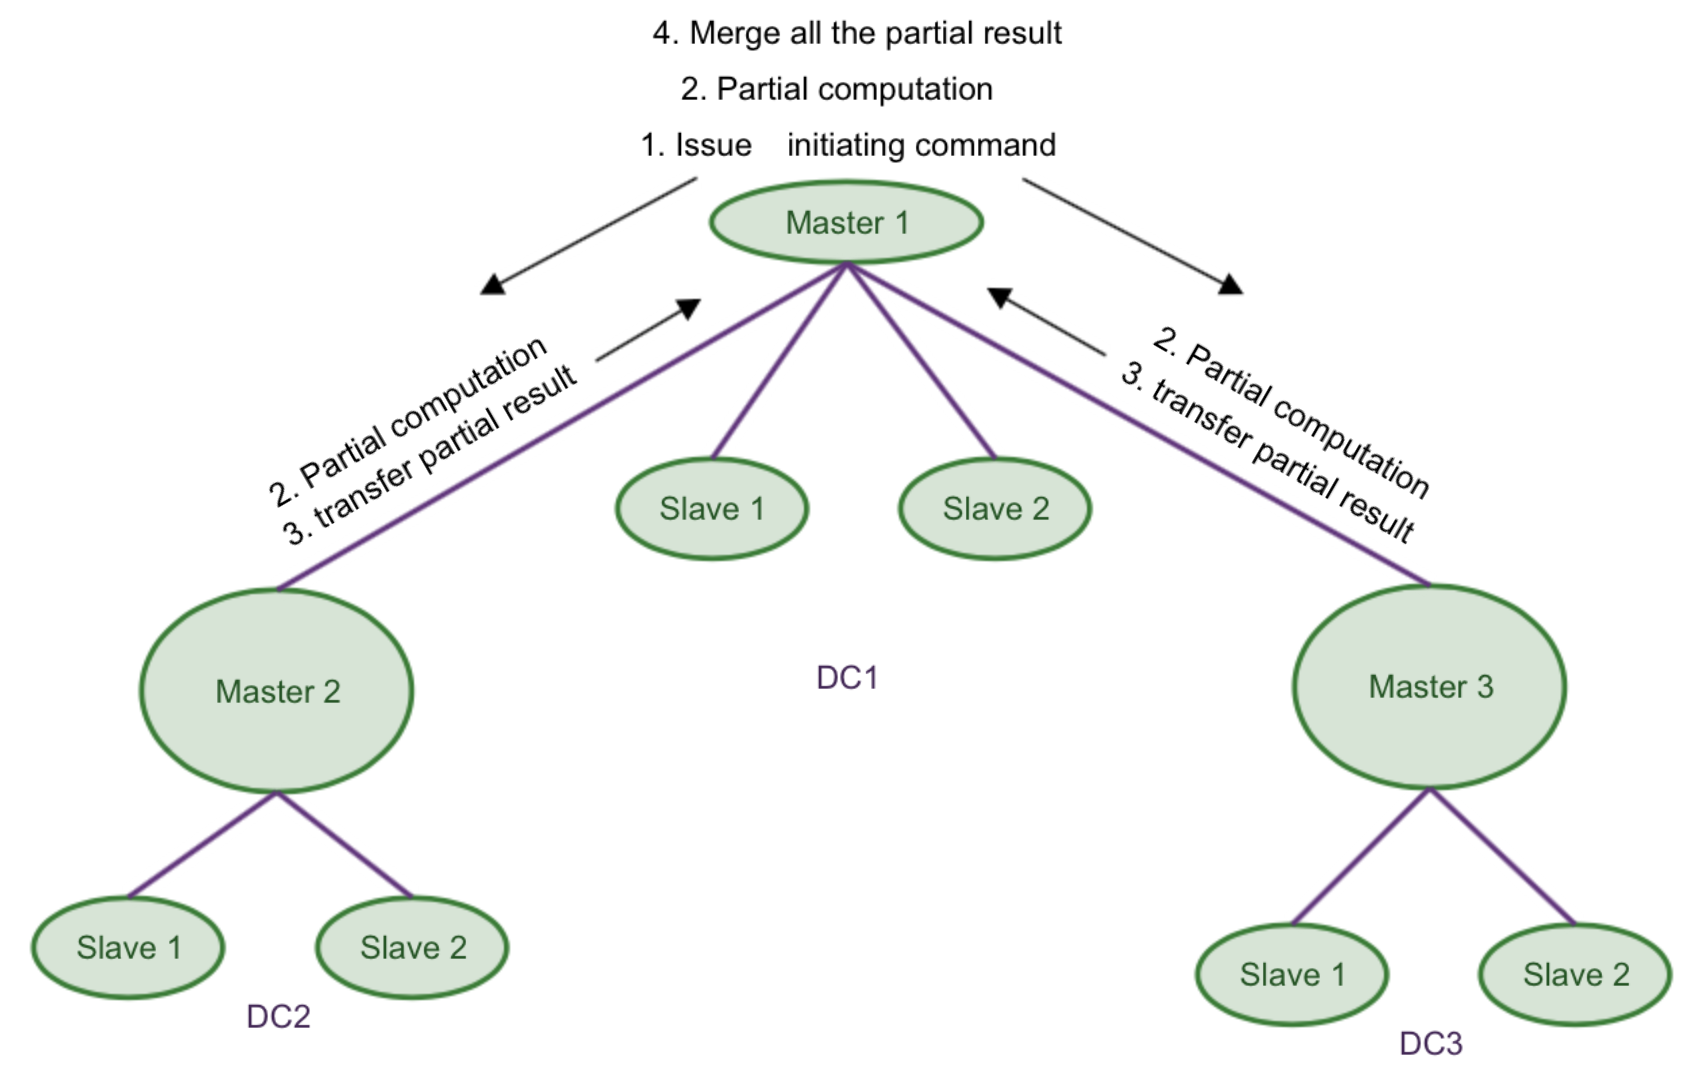
\includegraphics[width=5.2in]{learning.png}}
\caption{Graphical Interpretation of Learning Algorithm }
\label{learning}
\end{figure}

\newpage

\section{Our Implementation}
For the main program we used \emph{Hadoop MapReduce} framework. We used \emph{Java} as programming language. For inter data center communication we used \emph{Secure Shell (SSH)} Protocol. For some extra works we had to use \emph{C++} programming language also. 
\subsection{How the Distributed Algorithm Works}
A shell script initializes the whole learning process. Master node of every data center will contain this program file. Every data center will have the information of other data centers where data reside in distributed fashion. This program will read every other data center's information and with this information it will start another child program along with it's own information.

The child program receives information of all the data centers one by one. Then it will communicate with that data center and issue a command  to start it's internal computation for parameters to build a complete regression model.

The child process will match the information of two data centers passed to it. If it is the initiating data center, then it will start some master task. Other wise slave tasks will be initiated.

At first environment variables associated with \emph{Hadoop MapReduce} will be set up. At this point the main program of computing partial results will be executed on every data centers. The program is based on mapping input data into specific intermediate outputs and then reducing them. For example, while running the computation model of $\sum x^k$, the map function will map every $x$ into $x^k$ and send to the reducer. The corresponding reducer will sum all those   $x^k$ to generate $\sum x^k$. 

When the partial computational output is available in initiating data center, this program will rename the output files with appropriate names including corresponding data center information and move them into a common container. 

The main difference of non initiating data centers is rather than moving the renamed files this program will send those files to the common container. 

When all the partial computations are completed, the margin process will combine all the files of this container. 


\subsection{Runtime Analysis}
If the size of data is $n$, i.e. there are $n$ rows in every sample input then in the \emph{MapReduce} program, the number of maps for each parameter model will be $O(n)$. If the number of parameters to be generated is $p$ and number of machines is $\frac{p}{m}$ then the number of maps will be $O(mn)$\\
If the reducer of a parameter merges every two intermediate outputs of corresponding mapper then we can minimize the number of reducers to $O(\log _2 n)$. Therefore if the number of machines  is $\frac{p}{m}$, the number of reducers will be $O(m\log _2 n)$..

\section{Experimental Findings}
In case of finding any parameter, while any job is submitted it takes few time or its initial setup. For analyzing the result we ignored that  setup time by finding it empirically.
First of all we show the time vs data size graph. From Figure \ref{time vs size}, we can see that the time grows almost linearly with the size of data. 



\begin{figure}[!htbp]
\centering
\frame{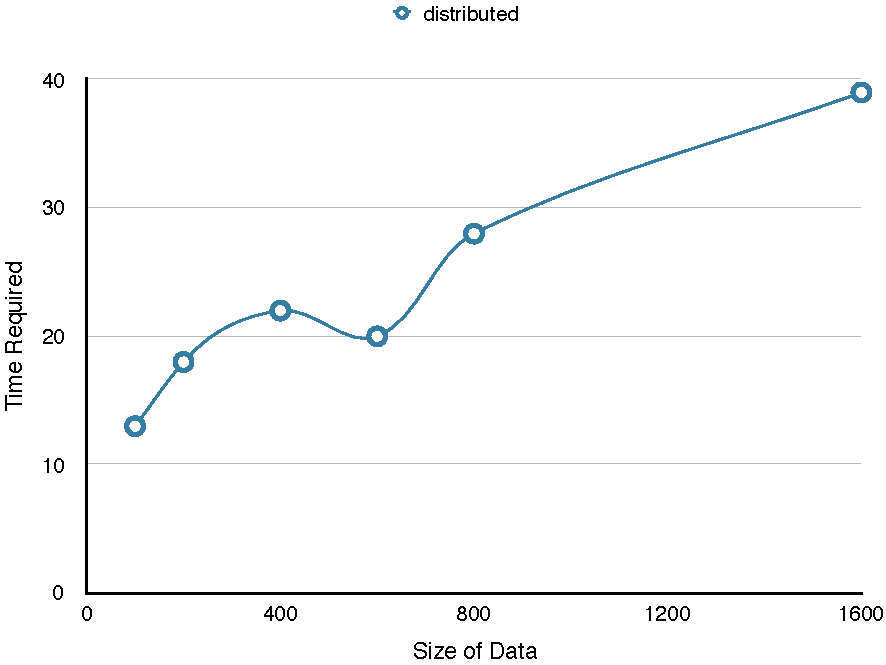
\includegraphics[width=5.2in]{dist.pdf}}
\caption{Time Required vs Data Size graph of our Distributed Approach}
\label{time vs size}
\end{figure}


A comparison between centralized approach and our distributed approach is shown in Figure \ref{cent vs dist}. We can easily see that time required for centralized approach is growing at a pretty high rate than that of the distributed approach.



\begin{figure}[!htbp]
\centering
\frame{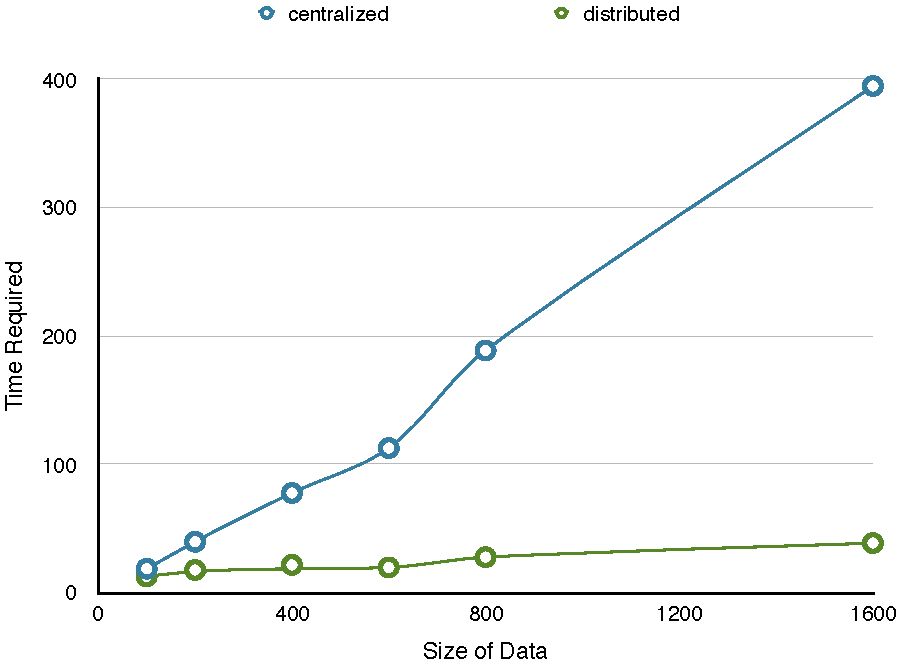
\includegraphics[width=5.2in]{centvsdist.pdf}}
\caption{Comparison graph between centralized and distributed approach}
\label{cent vs dist}
\end{figure}



As we were making an use of \emph{Model Parallelism}, the number of instances in a data center plays a big role in the computational runtime. We can demonstrate it by an example. 
\begin{itemize}
\item In case we have $n$ models to run and have $\frac{n}{k}$ instances in a data center. Then every instance will be assigned to run $k$ models. It means these $k$ models will run at a sequential basis. Obviously the number $k$ is preferable to be as low as possible.
\item The best result can be found with $k=1$. While the number of instances are equal to the number of models then every model can be run in parallel. Then the total runtime will be the  time  of the worst time taken model.  
\end{itemize}

As we were using free tires of $750$ hours in \emph{Amazon Web Services}, we did not have the scope to use as more instances as possible. In fact, we could  only use 3 instances at most for every data center. Still it showed a significant variance in runtime while running on different number of instances. In Figure   
\ref{instances}, we can see that the run time decreases as the number of instances increases.

\begin{figure}[!htbp]
\centering
\frame{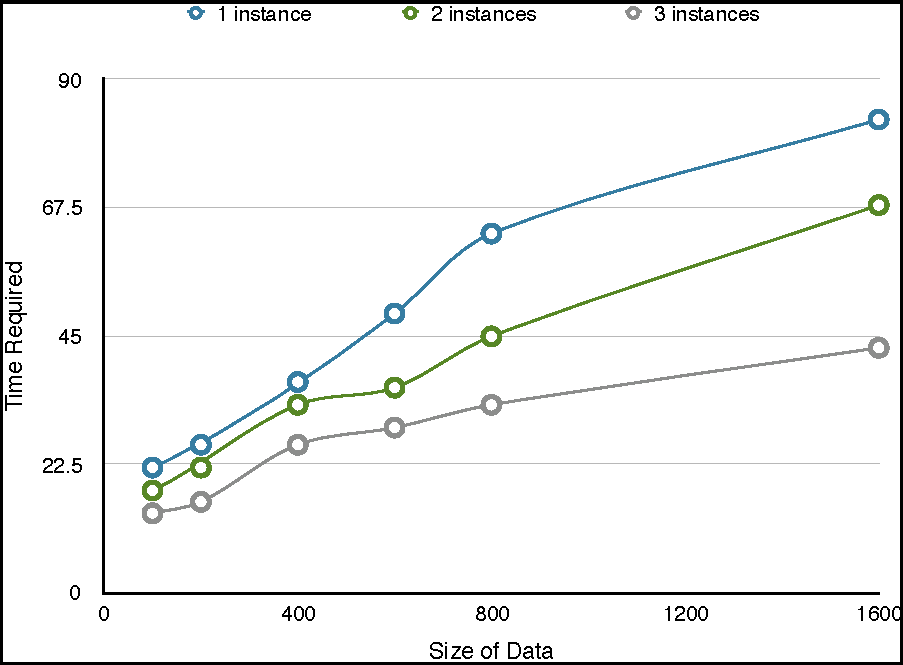
\includegraphics[width=5.2in]{instances.pdf}}
\caption{Comparison graph based on number of instances}
\label{instances}
\end{figure}



\newpage
\section{Limitations}
We used a general approach to create the regression models for both linear and polynomial regression. Each data center does its portion of computation on its own data. We applied the approach on mainly text input files where each file consisted of multi line texts. For each line we extracted 2 parameter as $x$ and $y$. Here we can see that we are finding sums such that $\sum x^2$, $\sum x^3$, $\sum y^2$, $\sum y^3$ etc. To be specific in order to create a linear regression model we need to calculate sums of exponents of $x$ and it was up to $\sum x^2$ then for polynomial it was up to $\sum x^4$. In general it can be observed that for a regression analysis of $n$th order we need to calculate up to $\sum x^{2n}$ and have to send $3n+2$ numbers of such summation values to a central data center. So we can see that using higher order regression analysis it will become practically impossible to use this approach. 

More problems arise while $x$'s carry large values. In case of polynomial regression if in general every data center has one billion $10^9$ line text input in data files and the average value of $x$ is in range $10^3$, then the system will have to handle sum values in the range of $10^{21}$. A different approach of handling such big numbers should be followed to make the approach more useful.   

The time required for the computations of parameters are not same. Primarily, in case of using \emph{Model Parallelism} if we have exactly same number of instances and models then we assume to have the best runtime. But all the models dont take the same time. As a result the load of running models can be further distributed among idle instances. Whenever any low time consuming model is finished in any instance, it becomes idle and any high time consuming model can be split and a portion can be assign to run in such idle instances.

\endinput

\chapter{Our Proposed Approach}
	\label{c:6}
As discussed before, we are interested in presenting an approach that will resolve the memory limitation problem and hence give an systematic way to run \emph{PPCA} on geographically distributed data. 

\section{Handling Tall and Wide Big Data}
Our first concern was to make commodity computers capable of performing PPCA on such big data which has very large sample count as well as very high dimension i.e. very large feature count. In this respect we will follow the approach from \cite{elgamal} with some necessary improvements. To have a distributed settings we will take advantage of cluster computing. In case of very wide data the size of principal subspace $W$ is going to be very big. Therefore, we have to treat the principal subspace $W$ as big data also. Performing PPCA in the conventional approach on tall and wide big data will result in the overflow of memory. Therefore, we have to make some kind of improvements to make the approach capable of handling tall and wide big data in case of performing PPCA overcoming the memory scarcity. The steps of performing PPCA in a single cluster is as follows:

\subsection{\textbf{Step 1 - Partition of Principal Subspace $W$}}\hspace*{\fill} \\
For data with the dimension $N \times D$ we will get a principal subspace of dimension $D \times d$ where $d$ denotes the number of principal components we want. Working with full horizontal $D$ dimension of $W$ will result in memory overflow. Therefore, we will make $n$ horizontal partition of $W$ and create $W_1, W_2, \dots , W_n$. As a result each stage of creating $W$ will consists of $n$ smaller stages of creating $W_i$. 


\subsection{\textbf{Step 2 - Data Partition}}\hspace*{\fill} \\
As we are partitioning the horizontal $D$ dimension of principal subspace $W$, we are indirectly make vertical partition of our data of $N \times D$. At each iteration of generating $W$, we have to work on a specific horizontal segment of it. Therefore, we have to work with only that segment of dimension of our data. In that sense we can say that we are creating vertical partition of our main data matrix. It might be a case that data is pretty large that even a distributed setting with multiple machines might not be capable of performing the PPCA task by keeping the full data in memory. In such case our approach can be memory efficient by loading only a single segment of data at each iteration. This will help in memory intense tasks.  

\subsection{\textbf{Step 3 - Expectation Step and Omission of Noise Model}}\hspace*{\fill} \\
From Algorithm \ref{basic} we can see that computation of $\pmb{\sigma ^2}$ involves $X$ which is going to a $N \times d$ matrix. Therefore, passing such big data will result in communication bottleneck. For simplicity of computation and minimizing the inter data cluster communication, we will omit the noise calculation. 

On the other hand, in order to take advantage from segmented computation, we have to make some changes in the Expectation and Maximization steps of the main \textbf{EM Algorithm} of PPCA. 
Omitting the noise model and from Equation (\ref{PPCA:EM}), (\ref{PPCA:EM1}) and Algorithm \ref{basic}, the E-Steps are:

\begin{align}
\label{1}
M &= W^T * W\\
\label{2}
X &= Y_c * W * M^{-1}\\
\label{3}
XtX &= X^T * X\\
\label{4}
YtX &= Y_c^T * X
\end{align}

In our approach $M$ is not going to be produces at the start of the process as ot depends on $W$ which will be segmented in our system. Therefore we are going to produce multiple number of $M$'s and accumulate them to produce the final $M$. The steps equivalent to Equation \ref{1}: 
\begin{align}
\label{5}
M_i &= W_i^T * W_i \\
\label{6}
M &= \sum^n_{i = 1} M_i
\end{align}
Similar thing will happen for producing $X$ of Equation \ref{2}:
\begin{align}
\label{7}
X_i &= {Y_c}_i * W_i\\
\label{8}
X &= \sum^n_{i = 1} X_i
\end{align}
%We can see that as soon as $M_i$'s and $X-i$'s are generated at the end of $n$ segmented iterations according to Equations \ref{5} and \ref{7}, we can generate $M$ and $X$ by using Equations \ref{6} and \ref{8}. Then Equation \ref{9} will be executed to produce final $X$
Steps to produce $XtX$:
\begin{align*}
    X   &= X * M^{-1}\\
    XtX &= X^T * X\\
        &= (X * M^{-1})^T*(X * M^{-1})\\
        &= {M^{-1}}^T*X^T*X*M^{-1}\\
        &= {(M^{-1})}^T*(X^T*X)*(M^{-1})
\end{align*}
Similarly we will produce $YtX$
\begin{align*}
    X   &= X * M^{-1}\\
    (YtX)_i &= {Y_c}_i^T * X\\
        &= ({Y_c}_i^T * X) * M^{-1} 
\end{align*}

\subsubsection{\textbf{Step 4 - Maximization Step}}\hspace*{\fill} \\
As we have mentioned earlier we are omitting the calculation of variance $\pmb{\sigma ^2}$. Therefore, our maximization step gets limited to the only computation of new $W$. As we are generating $W$ in a segmented approach, at iteration $i$ we are going to generate $W_i$ as follows:
\begin{equation*}
    Wi = (YtX)_i * XtX^{-1}
\end{equation*}
Here $(YtX)_i$ is the $YtX$ generated from $Y$ for the range of dimension corresponding to $i$.


\section{Flow Graph and IO Operations}
Figure \ref{flow_graph} shows the flow of the algorithm of handling tall and wide big data in a single cluster. The algorithm will start from a random state. It will randomly generate initial segments $W_1, W_2, \dots , W_n$. Then save them in  File System. At each round the algorithm will load a particular segment $W_i$ and with the corresponding dimensions of data $Y_i$ it will generate $M_i$ and $X_i$. after $n$ iterations complete $X$ and $M$ will be generated. Then using $X$, $M^{-1}$ and ${M^{-1}}^T$, it will generate $XtX$. At the same time using $Y_i$, $X$ and $M^{-1}$, it will generate particular $(YtX)_i$. Then using $XtX$ and $(YtX)_i$, the algorithm will generate new $W_i$ and store it in File System and then call the accumulation process to start for that particaulr $W_i$. \ref{tallnwide} is the Algorithm to handle tall and wide biog data in a single cluster while 

\begin{figure}[!htbp]
\centering
\frame{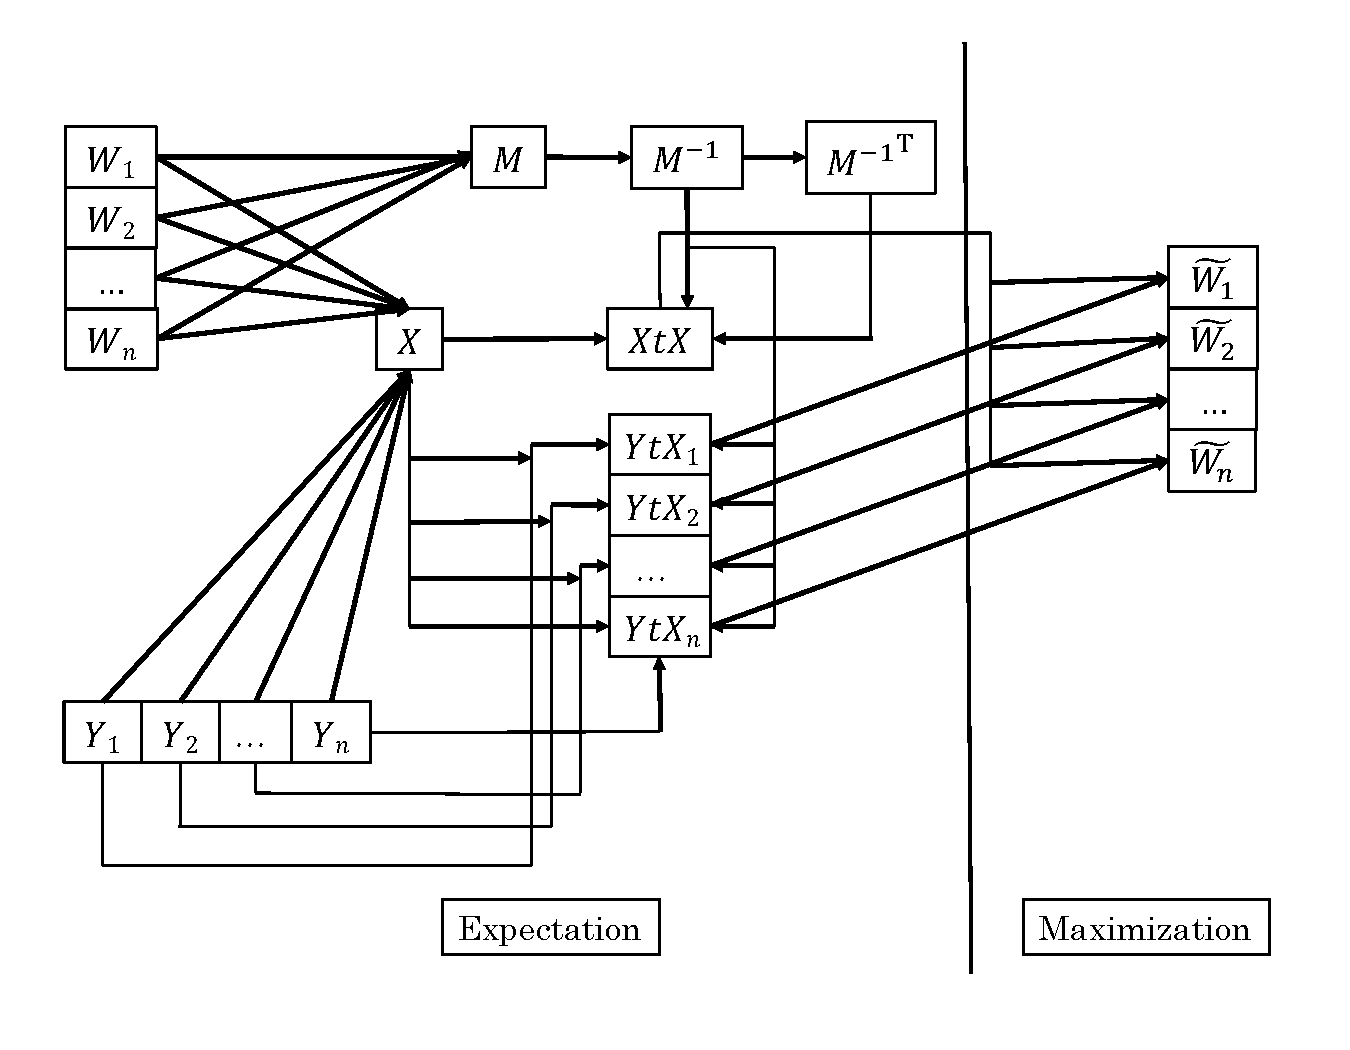
\includegraphics[width=5.5in]{flow.pdf}}
\caption{Flow Graph of Algorithm \ref{tallnwide}}
\label{flow_graph}
\end{figure}



\begin{algorithm} [!htbp]
  \caption{PPCA on Tall and Wide Big Data}
  \begin{algorithmic}[1]
  	\label{tallnwide}
  \STATE \textbf{createMyInfo()}
  \STATE $myInfo$ = \textit{readFile}($myInfo$)
  \STATE Let $Range[1.....partitionCount+1]$ be an array %containing range value of $W$ 
  \FOR {i from $1$ to $partitionCount$}
  	\STATE $Range[i] = (i-1)\times D \div partitionCount$
  \ENDFOR
  \FOR {i from $1$ to $partitionCount$}
  		\STATE $start$ = $Range[i]$  
		\STATE $end$ = $Range[i+1]$ 
		\STATE $W_i = $\textit{GenerateRandomW($start, end, d$)}
		\STATE \textit{saveWInStorage($W_i$)}
  \ENDFOR
  \STATE $Stop\_Condition$ = $False$
  \WHILE{($!(Stop\_Condition)$)}
  	  \STATE $M = null$ 
  \STATE $X = null$
	\FOR{i from $1$ to $partitionCount$}
		\STATE $start$ = $Range[i]$  
		\STATE $end$ = $Range[i+1]$  
		\STATE $W_i =$ \textit{loadWFromStorage}($start, end$)
		\STATE $M_{new} = W_i^T \times W_i$
		\STATE $M = M$ + $M_{new}$
		\STATE $X_m = Y_m \times W_i$
		\STATE \textbf{SegementedXJob($X, Y, X_m, W_i, start, end$)}
	\ENDFOR
	\STATE $invM = $\textit{invert($M$)}
	\STATE $YtX = null$
	\STATE $XtX = null$
	\FOR{i from $1$ to $partitionCount$}
		\STATE $s$ = $Range[i]$  
		\STATE $e$ = $Range[i+1]$  
		\STATE \textbf{generateYtXandXtX($YtX,XtX,X,Y,Y_m,i,s,e$)}
		\STATE $YtX = YtX \times invM$
		\STATE $XtX = invM^T \times XtX \times invM$
		\STATE $Wi = YtX \times $ \textit{invert($XtX$)}
		\STATE \textbf{startAccumulation($myInfo, i$)}
	\ENDFOR
  \ENDWHILE
  \end{algorithmic}
\end{algorithm}


\section{Accumulation of partial results from geographically distributed clusters}
As we mentioned earlier our data will be geographically distributed. That means we are not going to have any global view of data and no raw data passing is allowed to preserve national data sovereignty. Therefore, the partially computed results have to accumulated to produce the final result. We had the intention to minimize (a) the volume of data to be transmitted throughout the whole process and (b) accumulate the partial results in a way that will ensure the minimum accumulation time.
The former was handled in the previous subsection. In The later part we are going to be use some graph theory properties to achieve what we desire.

At each iteration of PPCA we are generating a segment of our principal subspace $W$. An arbitrary segment can can be denoted as $W_i$. Whenever one such segment is newly generated, each data cluster will call the \textbf{Accumulation} procedure from Algorithm \ref{accum}. The full accumulation process that we are proposing can be presented as follows:

\subsection{\textbf{Step 1: Generating The Initial Graph}}\hspace*{\fill} \\
The data clusters that are geographically distributed are connected by high or low bandwidth connection based on their location. According to \cite{nokia} and \cite{fujitsu}:
\begin{itemize}
\item Clusters that are located at the same region  generally have connection of bandwidth in the range above $100gbps$ 
\item Clusters that are located at nearby regions  generally have connection of bandwidth in the range of $10$-$100gbps$ 
\item Clusters that are located at different and distanced regions  generally have connection of bandwidth in the range of $1$-$10gbps$ 
\end{itemize}
At the start of the full PPCA process, every data cluster will check the bandwidth of the  connections of every other clusters it is connected with and generate a graph. The full process will results in a complete graph if there is an interconnection between every two data clusters. In this graph every node $v_i$ will represent a data cluster $DC_i$ while edge $e_{ij}(cost)$ between nodes  $v_i$ and  $v_j$ denotes that   $DC_i$ and $DC_j$ are connected at a b/w using which certain amount of data needs $cost$ amount of time to transmit among the two vertices. The Figure \ref{G} shows such a generated graph with $10$ data clusters.


\begin{figure}[!htbp]
	\centering
	\frame{\includegraphics[width=5.2in, page=3]{t.pdf}}
	\caption{Generated Graph $G$ According to Step-1}
	\label{G}
\end{figure}

\subsection{\textbf{Step 2: Generating MST}}\hspace*{\fill} \\
Using the graph generated in \textit{step 1}, every node will generate a \textit{Minimum Spanning Tree} to make a connected component with the least cost using time required to transmit data as the cost of the tree edges. 
Figure \ref{MST} shows the MST generated from graph from Figure \ref{G}.

\begin{figure}[!htbp]
	\centering
	\frame{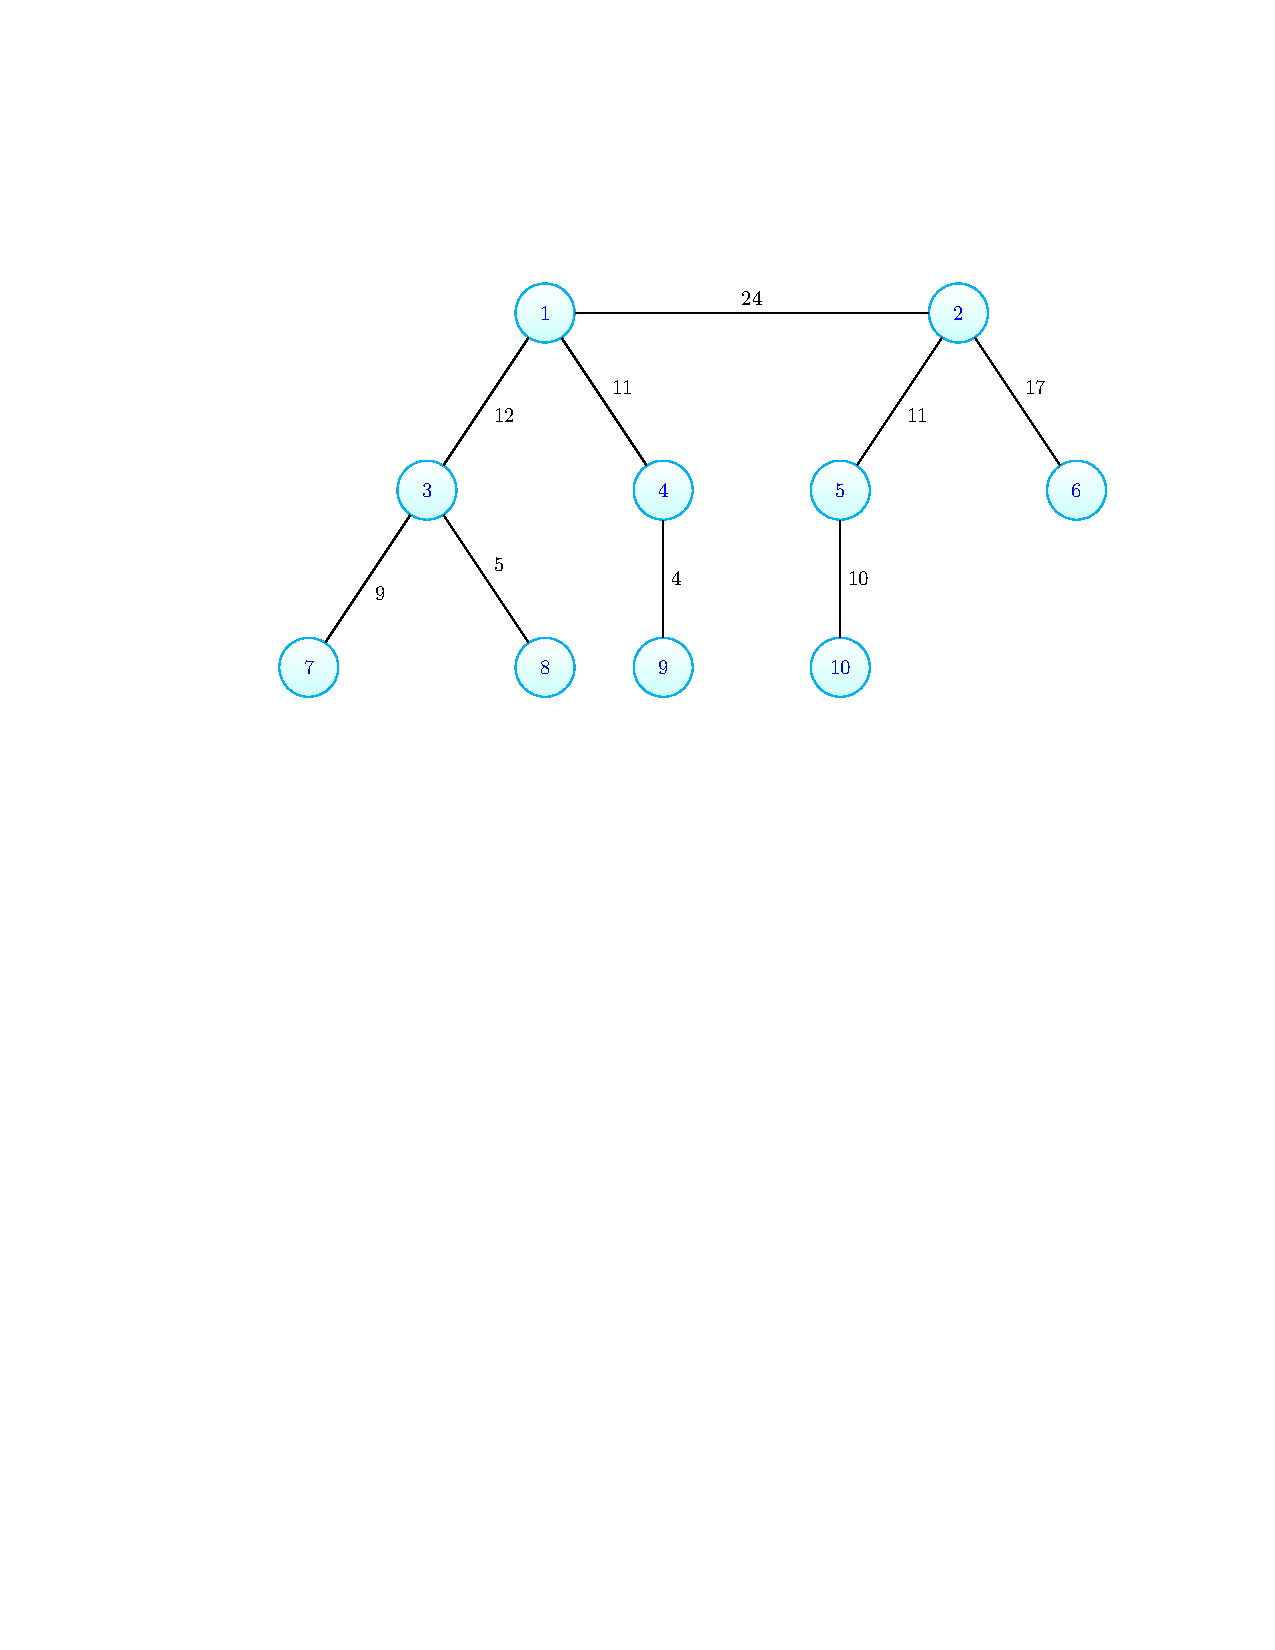
\includegraphics[width=5.2in, page=1]{t.pdf}}
	\caption{Generated MST According to Step-1 from Graph $G$}
	\label{MST}
\end{figure}


\subsection{\textbf{Step 3: Sub Tree Generation for Parallel Accumulation}}\hspace*{\fill} \\
We are going to generate two sub trees from the MST generated in \textit{Step 2} according to Algorithm \ref{algo6}. We will intended to choose the maximum time consuming edge $e_m$ and make a sub tree rooted at each of the end vertices of that edge. This will be done to make the process to use the maximum time consuming link only once while accumulating data. What we are trying to achieve is that all the data cluster nodes at each of the sub trees now can perform the accumulation task in parallel. Accumulation will be done in  bottom up direction. 
Therefore two accumulated results will  available at the two root data nodes. At that point a single exchange will results in having the final result at each of the root node of the two sub trees.

From this sub tree generation with using the node information, every data node will learn the information of its child nodes and parent nodes. During accumulation it will accumulate results from its child data nodes and notify the completion of it accumulation to its parent node.  

What we keep in mind that this  subtree formulation method might create some kind of unbalanced subtree. Figure \ref{uMST} shows such an unbalanced sub tree where $subtree1$ has a total cost of $51$ and $subtree1$ has a total cost of $21$.

\begin{figure}[!htbp]
	\centering
	\frame{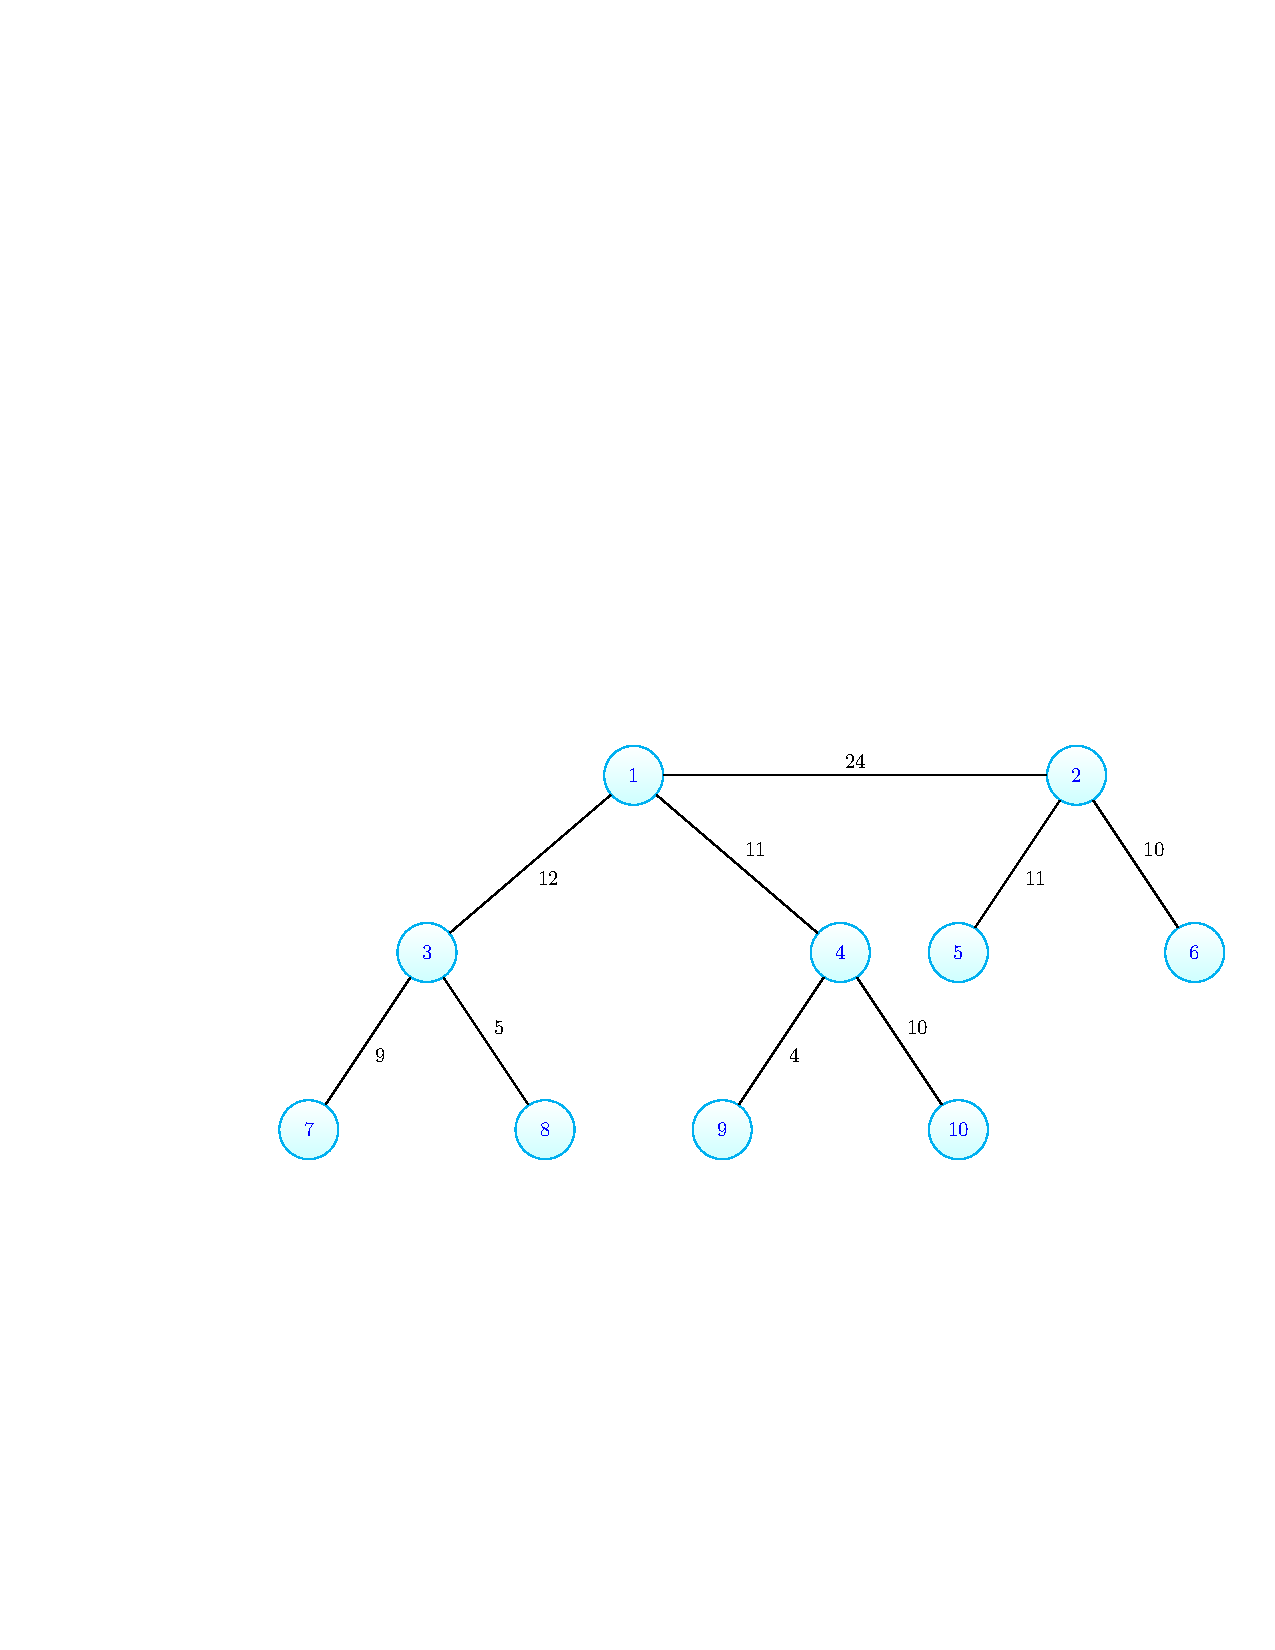
\includegraphics[width=5.2in, page=1]{t1.pdf}}
	\caption{Unbalanced Sub Tree}
	\label{uMST}
\end{figure}

To overcome such condition, we will then make a trade off between choosing the highest time consuming link and the balanced cost of the sub trees. To make the sub tree costs more or less balanced we will try to take the next maximum time consuming link and so on. 

\begin{algorithm} [!htbp]
	\caption{createSubTree}
	\begin{algorithmic}[1]
	\label{algo6}
		\STATE \textbf{Input: }$V_m$, Vertex Set of MST
		\STATE \textbf{Input:}	$E_m$, Edge Set of MST
		\STATE \textbf{Output: }$\{subTree1, subTree2\}$, Two Subtrees
		\STATE sort $E_m$ according to increasing b/w
		\STATE $done$=$Fasle$
		\WHILE{!$done$}
			\STATE $e$ = \textit{nextMinimumBWEdge($E_m$)}
			\STATE $v1$ = $e.startVertex$
			\STATE $v2$ = $e.endVertex$
			\STATE $subTree1$ = \textit{subTree($v1$)}
			\STATE $subTree2$ = \textit{subTree($v2$)}
			\STATE $cost1$ = \textit{cost($subTree1$)}
			\STATE $cost2$ = \textit{cost($subTree2$)}
			\IF{\textit{(max($cost1,cost2$)}/\textit{min($cost1,cost2$)}$ \leq 1.5$)}
				\STATE $done = True$
			\ENDIF
		\ENDWHILE	
		\STATE \textbf{return} $\{subTree1, subTree2\}$
	\end{algorithmic}
\end{algorithm}


\subsection{\textbf{Step 4: Redistribution of Final Accumulated Result}}\hspace*{\fill} \\
Whenever each of the root nodes completes the accumulation of its own sub tree, it will wait for the other root to complete. After that it will access the partially accumulated result from the other root node and complete the full computation. At this stage it will distribute the final result by pushing it through the links connecting to its neighbours. As there will be dedicated links, the result can be sent to each of the neighbours at the same time. Whenever ant node in a sub tree receives the final result it will also redistribute it to its child nodes in the tree configuration. The job will end with the leaf data nodes receiving the final accumulated result.

The Algorithm \ref{accum} is for accumulating the partial result. It will be called from every data nodes (leaf or non leaf) and according to the node information generated by Algorithm \ref{info} will communicate with other nodes in the communication tree.

\begin{algorithm} [!htbp]
\caption{startAccumulation}
	\begin{algorithmic}[1]
	\label{accum}
	\STATE \textbf{Input:} $myInfo$
	\STATE \textbf{Input:} $indexOfW$
	\STATE $W$ = \textit{loadW($indexOfW$)} 
	\FOR {(each $childNode$ in $myInfo.child()$)}
		\IF{($childNode.WisReady(indexOfW)$)}
			\STATE  $W_{child}$ = \textit{getWFromNode($childNode$)}
			\STATE $W$ = $W$+$W_{child}$
		\ENDIF
	\ENDFOR
	\STATE \textit{notifyParent($myInfo.parent$)}
	\IF {($myInfo.rootNode$)}
		\STATE Wait Until Other Root Node Data is Ready
		\STATE  $W_{otherRoot}$ = \textit{getWFromNode($myInfo.otherRootNode$)}
		\STATE $W$ = $W$+$W_{otherRoot}$
		\STATE Announce $doneW(indexOfW)$ as $True$
		\FOR {(each $childNode$ in $myInfo.child()$)}
			\STATE \textit{transmit($W$)}
			\STATE \textit{transmit($doneW(indexOfW)$)}
		\ENDFOR
	\ELSE
		\WHILE{(!$doneW(indexOfW)$)}
			\STATE \textit{wait()}
		\ENDWHILE
		\FOR {(each $childNode$ in $myInfo.child()$)}
			\STATE \textit{transmit($W$)}
			\STATE \textit{transmit($doneW(indexOfW)$)}
		\ENDFOR
	\ENDIF
	
	\end{algorithmic}
\end{algorithm}


\begin{algorithm}[!htbp]
	\caption{createMyInfo}
	\begin{algorithmic} [1]
	    \label{info}
	\STATE \textbf{Input: }$V: $ Set of Clusters as Vertices
	\STATE \textbf{Input: }$E: $ Set of Weighted Edges; b/w as Link Weights
	\STATE \textbf{Input: }$G=\{V,E\}$ Clusters' Distribution Graph
	\STATE $MST(V_m,E_m)$ = \textit{createMST($G$)}
	\STATE \{$subTree1, subTree2$\} = \textbf{createSubTree($V_m,E_m$)}
	\STATE $myInfo$ = \textit{createMyInfo($subTree1, subTree2, myID$)}
	\STATE \textit{saveMyInfo($myInfo$)}
	\end{algorithmic}
\end{algorithm}

\section{Communication Groups}
From the preceding subsections we can see that there will be two types of communication:
\begin{itemize}
\item \textbf{Local Communication}
This type of communication persists during the handling of tall and wide data in a single data cluster. Here all the slave data nodes of a single data cluster will work on a specific segment of the data matrix $Y$. While the single segment of $W$ will be available in every data node at a time. The master node will handle the partitioning of the data matrix while as well as the scheduling tasks. The slave nodes will work on their specific data segment and generate partial results that will be passed to the master node in order to generate the aggregated one. 
\item \textbf{Global Communication}
During the accumulation processes since $W_i$'s will be saved in the File System that will be under control of the master node in a data cluster only the master data nodes of different data clusters will communicate among themselves. This communication group is referred to as global communication group. 
\end{itemize}
The communication group are shown in Figure \ref{communication1}


\begin{figure}[!htbp]
    \centering
    \fbox{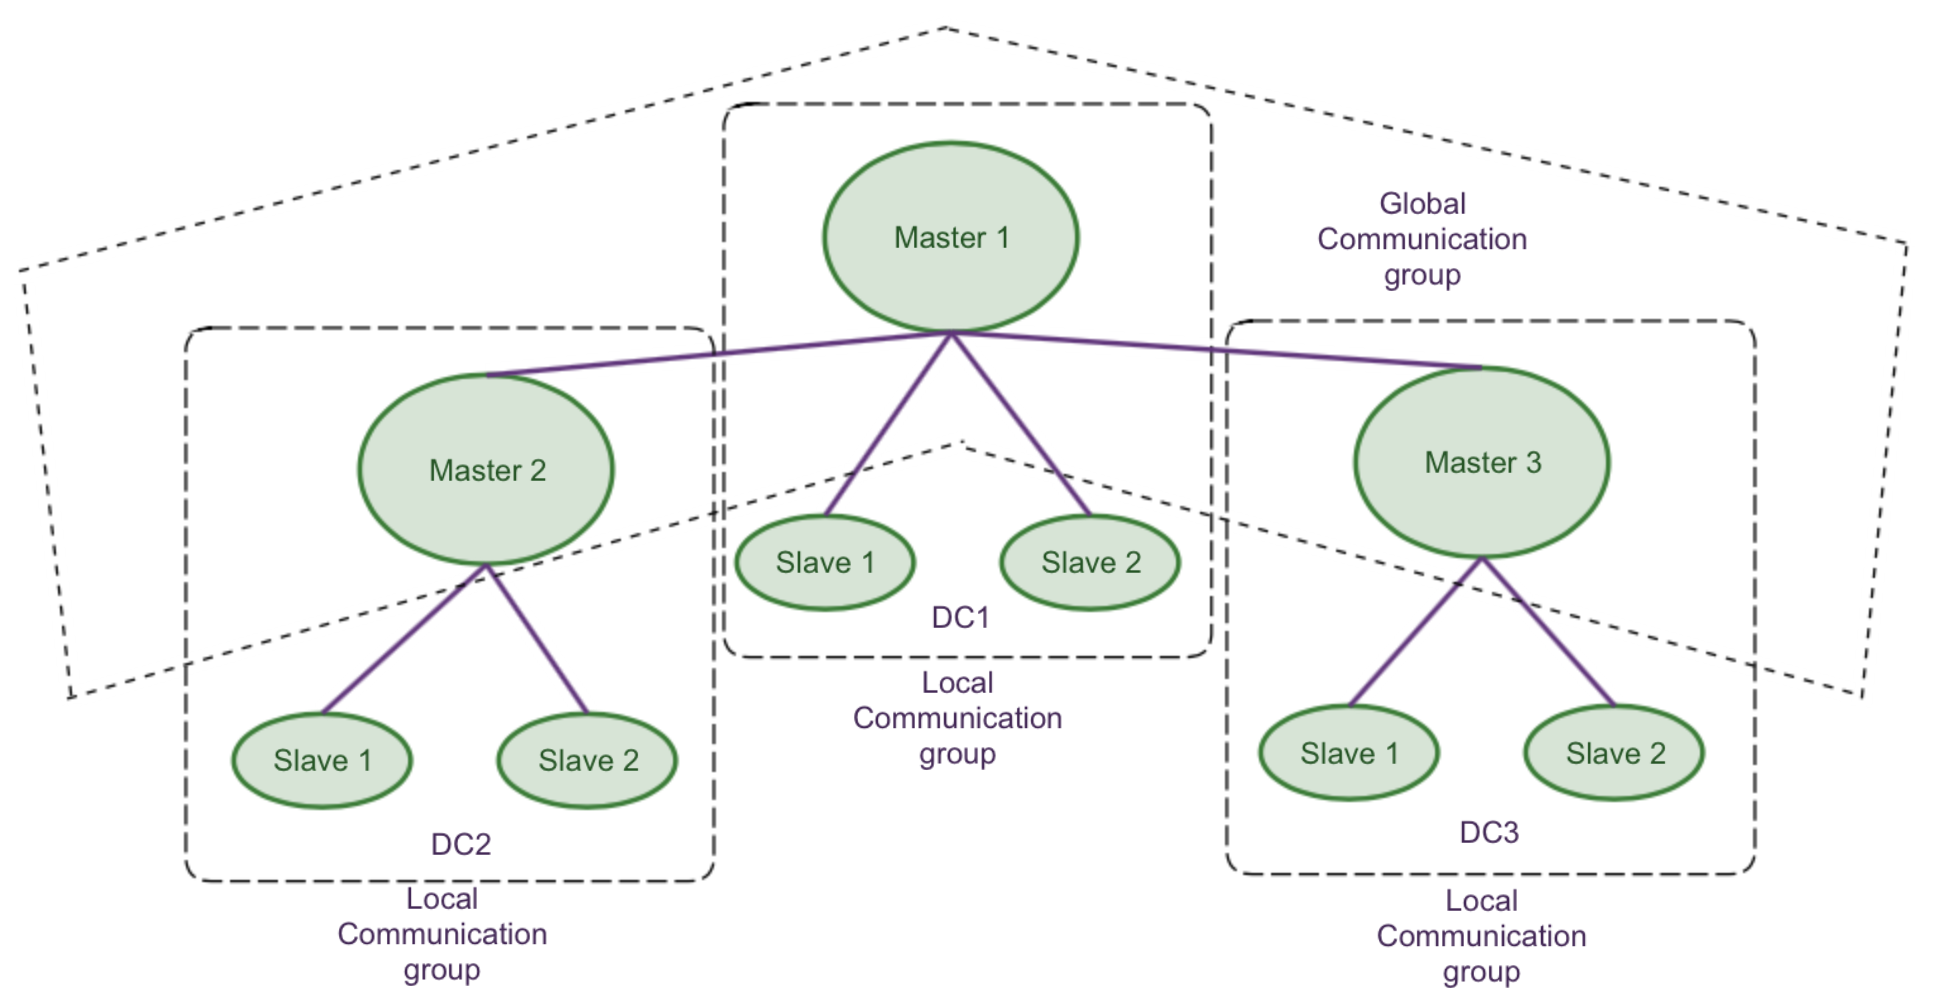
\includegraphics[width=5.2in]{communication.png}}
    \caption{Communication Groups in TallnWide and Accumulation}
    \label{communication1}
\end{figure}



\chapter{Properties of our Approach}
	\label{c:7}
In this section, we analyze the computational and communication complexity of our proposed algorithm and derive some theoretical properties.

\section{Computational Complexity}
We will discuss the computational complexity for Algorithm \ref{tallnwide} that do the task of computing principal subspace $W$ pf the input data $Y$. For computational complexity analysis, we will consider a spark-like \cite{spark} distributed setting where in a data cluster each of the data nodes has a portion of full data and intermediate results are stored in-core. Specifically if there are $c$ data nodes in a single cluster and each of them have approximately $N_i \times D$ data matrix $Y_i$, then we can write:
 $$Y = \sum _{i=1}^c Y_i$$
We assume the partition count of $W$ to be $p$. if every segment of $W$ is of size $D_i \times d$ where $d$ is number of principal components to be computed. Then we can write:
$$W = \sum _{i=1}^p W_i$$

Now our Algorithm \ref{tallnwide} has three different parts.

From line 7 to 12 a \textbf{For Loop} is generating initial random $W_i$'s. Here the running time is $\mathcal{O}(pD_id)$

From line 17 to 24 another \textbf{For Loop} is there to compute $X$ of Equation \ref{5} and \ref{6}. Here tasks of line 20-24 will have a time complexity of $\mathcal{O}(D_id^2+d^2+d+d+N_iD_id)$. That makes the aggregated runtime of this for loop $\mathcal{O}(pN_iD_id)$.

From line 29 to 37 another \textbf{For Loop} is generating $XtX$ and $YtX$, fining at generating new $W_i$. Therefore line 32-35 will have a time complexity of $\mathcal{O}(N_id^2 + D_iN_id+D_id^2+d^4 + D_id^2)$. That makes the aggregated runtime of this for loop $\mathcal{O}(pN_iD_id)$.

Therefore, if \textbf{While Loop} of line 14 runs for $r$ rounds then the total run time is going to be $\mathcal{O}(2rpN_iD_id)$.

\section{Communication Complexity}
The approach is highly communication intensive. At the end of generating each new segment of principal subspace $W$ each data cluster will call Algorithm \ref{accum} as a background process. This will make a data cluster to accumulate from its child nodes and give a notification to its parent. Each accumulation demands the transmission of a $D_i \times d$ matrix where $D_i$ varies with the number of partition is done on $W$. As partition information i.e. $D_i$ is available at the start of the process the communication tree generation can be done based on the available bandwidth between any two data clusters and the time required to transmit data of that size. For simplicity we assume the availability of dedicate bandwidth between any two data clusters.Under these assumptions, the time needed to make the accumulated result of a subtree available at the root node of that subtree is equal to the maximum aggregated time of any path from root to leaf node. If such paths are $P_1$ and $P_2$ of $subTree1$ and $subTree2$ respectively and maximum time consuming link time is $max\_time$, then the time of communication will be $$2*max\_time+2*max(time(P_1),time(P_2))$$ 
The $2$ is added as accumulated data will be redistributed in the same paths. In Figure \ref{fig:comm} the maximum time consumtioon link has a time of $27$ units the gray shaded paths has the maximum time consumption of $46$ and $31$ units. Therefore the communication time of accumulating one segement of $W$ will be $$2*27+2*max(46,31) = 146\ units$$ 

\begin{figure}
    \centering
    \frame{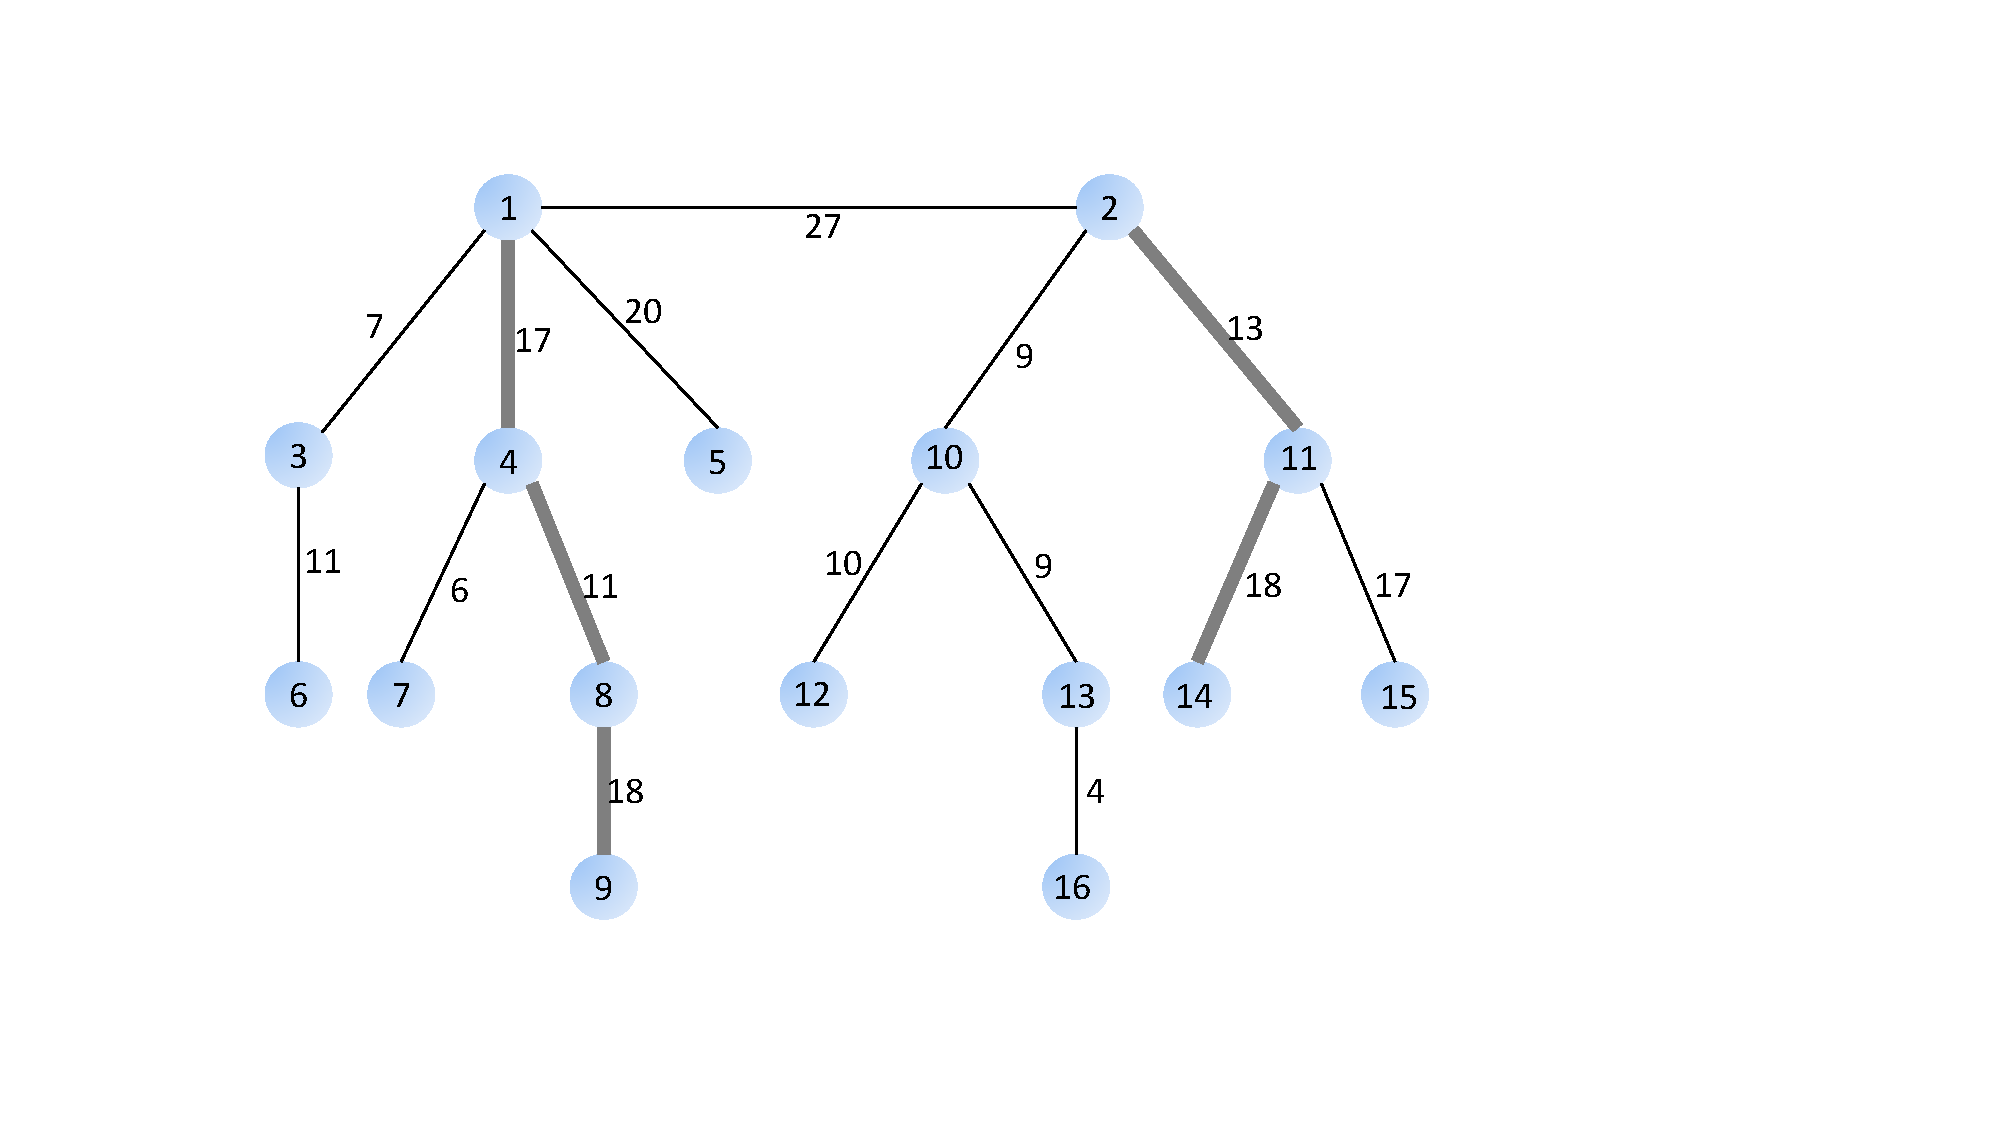
\includegraphics[width=5.2in]{com.pdf}}
    \caption{Communication Complexity}
    \label{fig:comm}
\end{figure}


\section{Stop Condition}
From Algorithm \ref{tallnwide} we can see that the \textbf{While} loop of line 14 will continue until the stop condition being true. While the algorithm will start we will set a tolerance rate. While the reconstruction error comes within the tolerance rate the algorithm will be considered to reach the convergence and eventually it will stop further iteration. The error checking formula is given by \cite{bishop}:
$e = ||Y -X * W^{-1}||_1$
However, since the sampling rate and size of data matrix will be varied, to make the eroor computing dependent of these  two, \textit{sPCA} \cite{elgamal} reported the norm of the reconstruction error divided by the norm of the matrix made up of the randomly selected rows, which is:
$$e=||Y_r - X_r*W^{-1}||_1/||Y_r||_1$$
Unfortunately the $W$ here is being generated as a whole but in our case we will be working on a particular segment of $W$. Therefore, We will have in hand a particular segment of $W$ namely $W_i$, a particular segment of $Y$ namely $Y_i$ and $X$ as a whole. This will break the data consistency and our calculated $e$ will be the desired one. Therefore, we were not able to compute original reconstruction error in this approach and examine the stop condition. Rather we used some approach used widely in Matlab. We checked the change in $W$ newly generated with the previous one and found the point of convergence by having a change in $W$ smaller than the tolerance. Initially we had two variables:
\begin{align*}
dw &= 0\\
maxWNew &= 0
\end{align*}
At the end of each iteration, These two variables will have their changed value and as soon as $dw$ is less than tolerance the algorithm will be considered to achieve convergence. 
\begin{align*}
maxWnew &= max(|{\widetilde{W}}_{pq}|, maxWnew)\ \forall p \in D, q \in d\\
dw &= max(|{W}_{pq} - {\widetilde{W}}_{pq} |, dw)\\
dw &= \dfrac{dw}{\sqrt{eps} + maxWnew}
\end{align*}

\begin{algorithm}
	\begin{algorithmic}[1]
	\label{stop}
	\caption{checkStopCondition}
	\STATE \textbf{Input:}$start$, $end$, $Wold$, $Wnew$, $stopCondition$, $dw$,  $maxWNew$, $tolerance$
	\FOR {$p$ = $start$ to $end$}
		\FOR {$q$ = $0$ to $nPC$}
		\STATE $maxWnew$ = \textit{max}(\textit{abs}($Wold[p-start][q]$), $maxWnew$)
		\ENDFOR
	\ENDFOR
	\FOR {$p$ = $start$ to $end$}
		\FOR {$q$ = $0$ to $nPC$}
		\STATE $maxWnew$ = \textit{max}(\textit{abs}($Wold[p-start][q] - Wnew[p-start][q]$), $dw$)
		\ENDFOR
	\ENDFOR
	\STATE $sqrtEps$ = 2.2204e-16
	\STATE $dw$ = $dw /$ ($sqrtEps + maxWnew$)
	\IF {$dw \leq tolerance$}
		\STATE $stopCondition$ = $True$
	\ENDIF
	\end{algorithmic}
\end{algorithm}

\chapter{Implementation in Spark Cluster System}
	\label{c:8}
We implemented our proposed system on Spark \cite{spark} cluster computing system. Spark gives us various types of storage system. Spark provides resilient distributed datasets (RDDs) and parallel operations on these datasets. Resilient Distributed Datasets (RDD) is a fundamental data structure of Spark \cite{spark-site}. It is an immutable distributed collection of objects. Each dataset in RDD is divided into logical partitions, which may be computed on different nodes of the cluster. From user level the persistanc of RDD can be controlled. It can be cached in memory or store on disk to be used later through IO operations. Moreover the user can control its partitioning process like partition by key.

In case of small data that can be kept in memory while computing, we did the in-memory computations by making the input matrix $Y$ persistent in the memory of the machines of our spark cluster. Therefore we could perform faster distributed operations on our data. On the other hand, for clusters with small count of nodes i.e. small amount of memory, we have to make IO operations by keeping the data on disks and load a specific segment of it while needed. 
The Algorithms \ref{segmented1} and \ref{segmented2} are based on the Spark Programming. 







\begin{algorithm} [!htbp]
  \caption{SegmentedXJob($X,Y,X_m,W,start,end$)}
  \begin{algorithmic} [1]
\label{segmented1}
	\STATE $Y_nX$ = $Y$.zip($X$)
	\STATE $X$ = $Y_nX$.map\{($Y_nX$)$_i \Rightarrow$
	        \STATE \tab $Y_i$ = ($Y_nX$)$_i$.\textit{arg0()}.\textit{range}($start,end$)
			\STATE \tab $X_i$ = ($Y_nX$)$_i$.\textit{arg1()}
			\STATE \tab dotRes = $Y_i \times W$
			\STATE \tab $X_i$ = $X_i$ + dotRes - $(X_m)_i$
			\STATE \}
  \end{algorithmic}
\end{algorithm}



\begin{algorithm} [!htbp]
  \caption{SegmentedXJob($YtX,XtX,X,Y,Y_m,i,s,e$)}
  \begin{algorithmic} [1]
\label{segmented2}
	\STATE $Y_nX$ = $Y$.zip($X$)
	 \IF{($i == 1$)}
	 		\STATE $YtXSum = spark.accumultor(newMatrix(D,d))$
			\STATE $XtXSum = spark.accumultor(newMatrix(D,d))$
	 		\STATE $Y_nX$.map\{($Y_nX$)$_i \Rightarrow$
	 		\STATE \tab $Y_i$ = ($Y_nX$)$_i$.\textit{arg0()}.\textit{range}($s,e$)
			\STATE \tab $X_i$ = ($Y_nX$)$_i$.\textit{arg1()}
			\STATE \tab $(YtX)_i$ = $Y_i^T \times  X_i$ - $Y_m^T \times X_i$   
			\STATE \tab $(XtX)_i$ = $X_i^T \times  X_i$
			 \STATE \tab $YtXSum$.\textit{add($(YtX)_i$)}
			 \STATE \tab $XtXSum$.\textit{add($(XtX)_i$)}
			\STATE \}
		\STATE $YtX = YtXSum$.\textit{value()}
		\STATE $XtX = XtXSum$.\textit{value()}
	\ELSE
			\STATE $YtXSum = spark.accumultor(newMatrix(D,d))$
	 		\STATE $Y_nX$.map\{($Y_nX$)$_i \Rightarrow$
			\STATE \tab $Y_i$ = ($Y_nX$)$_i$.\textit{arg0()}.\textit{range}($s,e$)
			\STATE \tab $X_i$ = ($Y_nX$)$_i$.\textit{arg1()}
			\STATE \tab $(YtX)_i$ = $Y_i^T \times  X_i$ - $Y_m^T \times X_i$   
			 \STATE \tab $YtXSum$.\textit{add($(YtX)_i$)}
			\STATE \}
		\STATE $YtX = YtXSum$.\textit{value()}
	 \ENDIF
  \end{algorithmic}
\end{algorithm}

\chapter{Experimental Evaluation}
	\label{c:9}
In this chapter we will present our experimental result that we found while implementing our approach in \textit{Spark} Cluster computing system.
\section{Cluster Setup}
We built \textit{Spark} clusters in our \textit{Undergraduate Thesis Lab}. To evaluate the performance of the method to handle \textit{Tall and Wide Big Data}, we created clusters that was composed of three machines with one master node and two slave nodes. Each of the machines had $64GB$ of memory and quad core processor of $3.6GHz$. That makes our cluster with $12$ cores of processor to work with. We installed \textit{Apache Spark 2.0} with \textit{\textit{Hadoop} 2.7} for \textit{HDFS}.

On the other hand, to test the accumulation process, we created 8 spark clusters each of which contained only one slave node. as we did not have that amount of machines in a single cluster, we used small dimensional data to test this part of the method.




\section{Data Sets}
We use two real datasets. These data sets contains data of different types and of different sizes. The dimensionalities are also different. The datasets are:

\begin{itemize}
\item \textbf{Amazon Product Ratings}\hspace*{\fill} \\
This data set is from \textit{Amazon} web sites that includes the user ratings on various products items. In the raw data, it contains three columns: 1) unique User ID, 2) unique Product ID, 3) Product Rating. To make it easily fit in our system we gave each of the User ID and Product ID a number. There was $21\ millions$ user id's and $9\ millions$ product id's. That makes it $21M \times 9M$ sparse data matrix. In the matrix if cell ($x,y$) have a number $z$, that means user $x$ has given a rating $z$ to the product $y$. The raw data was of size $4.73GB$
\item \textbf{Twitter Follower Relationship}\hspace*{\fill} \\
This data set is of \textit{Twitter} that includes the follower information of every user ID. The raw data has two columns: two User IDs. The first User ID is followed by the second one. The maximum user Id is $61578414$. That makes it a data set where every data sample has a dimension of $61M$ while it has $61M$ rows that makes it a data set of $61M \times 61M$. a $1$ in cell $(x,y)$ indicates that user $y$ follows user $x$ while a $0$ indicates the negatively. The raw data was of size $26.17GB$
\end{itemize}

\section{Performance Metrics}
We did not have much opportunity to compare our method with others as there are no other algorithm that can handle geo-distributed tall and wide big data. Though the \textit{sPCA} \cite{elgamal} showed some kind of implementation of PPCA in a distributed cluster, it also fails to run on very large dimensional data. Moreover, it has no method to accumulate partial data from different geographic locations. 

\subsection{Partition Count of $W$}
In case of handling Tall and Wide data in a single cluster we made partitions of the principal subspace $W$. However, one of the limitations of our method is that we could not find a optimum partition count based on the data size and available resources. Rather we gathered some empirical results by giving manual input on the partition count. Table \ref{tab:amazon_partition} shows the influence of no of partitions on the total running time and IO operation time of the data matrix of \textit{Amazon Product Rating} Dataset. As at a time, we are working on a single partition of $W$ and also creating a single partition of $W$, we had to allow IO operations. We had to load and store $W_i$ while working on 
the range of dimension of our data matrix $Y$ corresponding to the subscript $i$. Table \ref{tab:twitter_partition} shows the same information for data matrix of \textit{Twitter Follower} Dataset.

\begin{table}[!htbp]
    \centering
    \begin{tabular}{|c|c|c|c|c|c|}
    \hline
    Memory &Data Size &Partitions &Iterations &Runtime &IO Time \\
    \hline
    \multirow{4}{17pt}{$6GB$}  & \multirow{4}{7em}{$21M \times 9.8M$} &15  &7		&18.0 Hrs   	  &65 Mins\\
    \cline{3-6}
         & & 13 &8		&18.5 Hrs   	  &50 Mins\\
    \cline{3-6}
         & & 11 &7		&14.1 Hrs   	  &44 Mins\\
    \cline{3-6}
         & & 10 &\multicolumn{3}{|c|}{Failed} \\
    \hline
    
    \multirow{4}{17pt}{$8GB$}  & \multirow{4}{7em}{$21M \times 9.8M$} &12  &8		&9.8 Hrs   	  &61 Mins\\
    \cline{3-6}
         & & 11 &7		&9.5 Hrs     	  &57 Mins\\
    \cline{3-6}
         & & 10 &6		&5.5 Hrs   	  &50 Mins\\
    \cline{3-6}
         & & 9 &\multicolumn{3}{|c|}{Failed} \\
    \hline
    
    \multirow{4}{17pt}{$8GB$}  & \multirow{4}{7em}{$10M \times 7M$} &9  &8		 &5.3 Hrs   	  &41 Mins\\
    \cline{3-6}
         & & 8 &7		 &4.1 Hrs    	  &38 Mins\\
    \cline{3-6}
         & & 7 &\multicolumn{3}{|c|}{Failed} \\
    \hline
    \multicolumn{6}{c}{}
    \end{tabular}
    \caption{Effect of Partition count of $W$ on Amazon Data Set }
    \label{tab:amazon_partition}
\end{table}

\begin{table}[!htbp]
    \centering
    \begin{tabular}{|c|c|c|c|c|c|}
    \hline
    Memory &Data Size &Partitions &Iterations &Runtime &IO Time \\
    \hline
    \multirow{4}{17pt}{$8GB$}  & \multirow{4}{7em}{$61M \times 61M$} &22  &6		&91.1 Hrs   	  &345 Mins\\
    \cline{3-6}
         & & 20 &7		&108.5 Hrs   	  &397 Mins\\
    \cline{3-6}
         & & 19 &\multicolumn{3}{|c|}{Failed} \\
    \hline
    
    \multirow{4}{17pt}{$12GB$}  & \multirow{4}{7em}{$61M \times 61M$} &20  &8		&99.3 Hrs   	  &405 Mins\\
    \cline{3-6}
         & & 18 &7		&87.4 Hrs   	  &317 Mins\\
    \cline{3-6}
         & & 17 &\multicolumn{3}{|c|}{Failed} \\
    \hline
    \multicolumn{6}{c}{}
    \end{tabular}
    \caption{Effect of Partition count of $W$ on Twitter Data Set }
    \label{tab:twitter_partition}
\end{table}

\subsection{Running Time}
We compare our Spark implementation with \textit{sPCA}. It should be noted that for higher dimensional data \textit{sPCA} will fail to run. As a result, we will not be able to make a comparison for such data samples.

\subsubsection{Time to Achieve Target Accuracy}
We compare our spark implementation with sPCA-Spark based on the time needed to reach our desired convergence point. We varied the size of the input dataset in two ways 1) change dimension size for fixed sample count and 2) change sample count for a fixed dimesnion size. Then we measured the time needed for our implementaion as well as \textit{sPCA-Spark}. The comparison results is shown in Figures \ref{comp:N} and \ref{comp:D}. We used the dataset of \textbf{Amazon Product Ratings}.

In Figure \ref{comp:N} we varied the sample count of the input data matrix. However, we kept the same dimension i.e. column count ($80$ thousands in number). The figure shows that the running times for our implementation is higher than that of the \textit{sPCA}. We had a different approach of implementation that increases the sequential tasks in our algorithm. We had to make this trade off in order to handle the higher dimension of data. 

\begin{figure}[!htbp]
    \centering
    \frame{\includegraphics[page=2]{res.pdf}}
    \caption{Running Time per Iteration Comparison for Amazon data for $D=0.08M$}
    \label{comp:N}
\end{figure}

In Figure \ref{comp:D} we varied the dimension of each sample of the input data matrix. However, we kept the sample count i.e. row count ($21$ millions in number). The figure shows that the running times for our implementation is little bit higher than that of \textit{sPCA}. However \textit{sPCA} failed to run for data with dimension larger than $140K$ and our algorithm was successful to perform PPCA on data with those higher dimension showed in the graph. The graph shows dimension up to $2M$ while for this dataset we run our algorithm for data with dimension up to $9.8M$. 

 
\begin{figure}[!htbp]
    \centering
    \frame{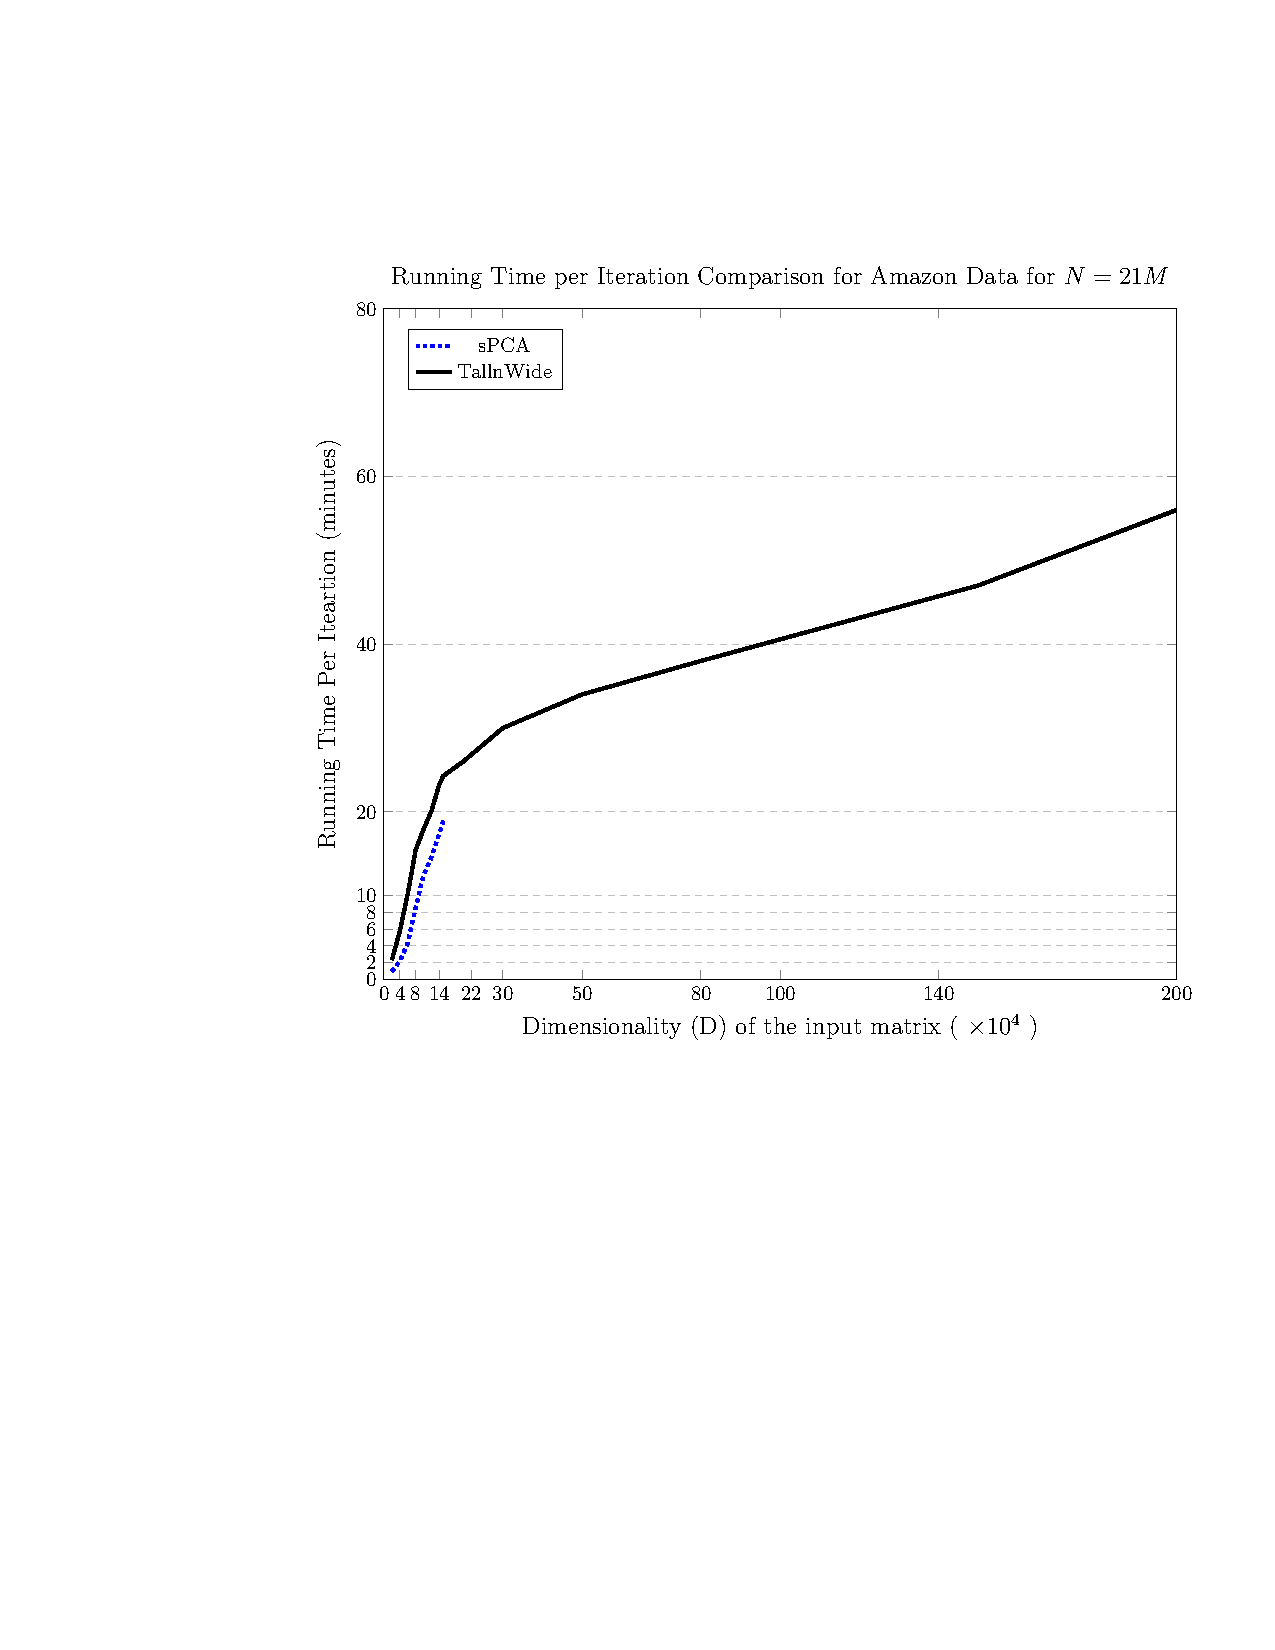
\includegraphics[page=1]{res.pdf}}
    \caption{Running Time per Iteration Comparison for Amazon Data for $N=21M$}
    \label{comp:D}
\end{figure}


\newpage
Same two comparison on Twitter daata set are shown in Figure \ref{comp:N1} and \ref{comp:D1}
\begin{figure}[!htbp]
    \centering
    \frame{\includegraphics[page=4]{res.pdf}}
    \caption{Running Time per Iteration Comparison for Twitter data \textit{sPCA} with  $D = 0.05M$}
    \label{comp:N1}
\end{figure}

\begin{figure}[!htbp]
    \centering
    \frame{\includegraphics[page=3]{res.pdf}}
    \caption{Running Time per Iteration Comparison for Twitter Data for $N = 65M$}
    \label{comp:D1}
\end{figure}

\newpage
\subsubsection{Memory Usage}
Figure \ref{comp:mem} shows the memory utilization during the generation of a single segment of $W$ on Amazon Data Set. The graph is shown for $N=21M$. The algorithm was run on $8GB$ memory. In the graph any segment count on the left of the left most point on each curve willl result in failure of execution. It also shows that memory utilization becomes saturate at minimum of around $2GB$ as the segment count converges to $17$ in this setup. 
\begin{figure}[!htbp]
    \centering
    \frame{\includegraphics[page=5]{res.pdf}}
    \caption{Intermediate Data Size for Amazon Data for $N=21M$ and memory = $8GB$}
    \label{comp:mem}
\end{figure}

\chapter{Conclusion}
	\label{c:10}
In this chapter we draw our concluding remarks and some future works that can possibly improve our present work at  a large scale.
\section{Concluding remarks}
In this paper, we tried to analyze various issues of computing the principal components of an input data matrix which has large number of data samples while each of the samples has very large dimension. We characterized this kind of data as \textit{Tall and Wide Big Data}. In addition the data is distributed at different geographic locations. Our analysis also indicated that the present algorithms for performing \textit{PCA} are not capable of performing the task on such data sets. We presented a new approach and implementation for PCA that is capable of handling big data with very large dimension and can accumulate the partial results from different geographic locations in an efficient way. Our approach is based on the probabilistic PCA (PPCA) algorithm defined in \cite{bishop}. We implemented this method on Spark platform and showed that it did the job significantly well.  
\section{Future Works}
There are some issues that we were not capable of solving. Therefore, in future these issues can be handled to make our method a more effective one.
\subsection{Capability of Computing Accuracy and Error}
As stated earlier we could not calculate the error and accuracy. In \cite{elgamal}, they measure the accuracy by computing the 1-Norm of the reconstruction error, which is given by: $e = ||Y -X * W^{-1}||_1$. Although this provides a common way to compare the accuracy of different algorithms, the reconstruction error is a big, dense matrix which is costly to store and process. They reduce the cost of storage by computing the error row by row, avoiding the need to store the large reconstruction matrix in the file system. Nevertheless, iterating over the resulting dense rows is still time consuming. They reduce this time by measuring the error only on a random subset of the rows. To have a unique way to interpret the measured error, independent of the sampling rate or matrix size, they report the norm of the reconstruction error divided by the norm of the matrix made up of the randomly selected rows, which is:
$$e=||Y_r - X_r*W^{-1}||_1/||Y_r||_1$$
In addition, they measure the ideal accuracy that can be achieved with 50 principal components after a large number of iterations. After each iteration, they report the percentage of the ideal accuracy that is achieved.

However, in our case as we are working with very large sized data and so even after applying all the improvements, we failed to find the actual error and accuracy. Therefore, we had to use different approach to check the convergence.
\subsection{Designing Better Stop Condition}
The stop condition was not that much up to the mark in our method. As we were not able to find the actual accuracy and error rate, it results in an alternative approach in stop condition. However, using current accuracy and actual accuracy ratio a better stop condition can be designed.
\subsection{Designing Optimum Partition Count of Principal Subspace $W$}
In case of handling Tall and Wide data in a single cluster we made partitions of the principal subspace $W$. However, one of the limitations of our method is that we could not find a optimum partition count based on the data size and available resources. Rather we gathered some empirical results by giving manual input on the partition count. In future it would be a good work to find a formula to calculate the minimum number of partition at which the cluster  can handle that particular wide data.
\subsection{Improved Implementation for Dense Matrix Data}
We did our evaluation on sparse matrix. However, we did not give proper and optimized implementation for dense matrices. In future we intend to do the optimization so that it can handle tall and wide dense data also.

\endinput

% Bibliographies and appendices
%\begin{thebibliography}{1}

\bibitem{1}
Matei Zaharia et al. Resilient distributed datasets: A fault-tolerant abstraction for in-memory cluster computing. In NSDI, 2012.


\bibitem{2}
Yucheng Low et al. Distributed GraphLab: A Framework for Machine Learning and Data Mining in the Cloud. PVLDB, 2012.

\bibitem{3}
Mu Li et al. Scaling distributed machine learning with the parameter server. In OSDI, 2014.

\bibitem{4} 
Ashish Thusoo et al. Data warehousing and analytics infrastructure at Facebook. SIGMOD, 2010.

\bibitem{5}
George Lee et al. The unified logging infrastructure for data analytics at Twitter. PVLDB, 2012.

\bibitem{6}
Aditya Auradkar et al. Data infrastructure at linkedIn. In ICDE, 2012.

\bibitem{7}
Ariel Rabkin et al. Aggregation and degradation in jetstream: Streaming analytics in the wide area. In NSDI, 2014.

\bibitem{8}
Ashish Vulimiri et al. Global analytics in the face of bandwidth and regulatory constraints. In NSDI, 2015.

\bibitem{9}
Nikolaos Laoutaris et al. Inter-datacenter bulk transfers with netstitcher. In SIGCOMM, 2011.

\bibitem{10}
Albert Greenberg et al. The cost of a cloud: research problems in data center networks. SIGCOMM, 2008.

\bibitem{11}
Martin Rost and Kirsten Bock. Privacy by design and the new protection goals. DuD, January, 2011.

\bibitem{12}
European Commission press release. Commission to pursue role as honest broker in future global negotiations on internet governance. \url{http: //europa.eu/rapid/press-release IP-14-142 en.htm}.

\bibitem{13}
Principal component analysis: \url{https://en.wikipedia.org/wiki/Principal_component_analysis}.

\bibitem{14}
J. Shlens. A tutorial on principal component analysis. \textit{arXiv preprint
arXiv:1404.1100}. 2014.

\bibitem{elgamal}
T. Elgamal and M. Hefeeda. Analysis of pca algorithms in distributed environments. \textit{arXiv preprint arXiv:1503.05214}. 2015.

\bibitem{16}
N. P. Halko. Randomized methods for computing low-rank approx- imations of matrices. Ph.D. dissertation, Boulder, CO, USA, 2012, aAI3507998.

\bibitem{17}
M. E. Tipping and C. M. Bishop. Probabilistic principal component analysis. \textit{Journal of the Royal Statistical Society: Series B (Statistical Methodology), vol. 61, no. 3, pp. 611?622}. 1999.

\bibitem{18}
S. Roweis. Em algorithms for pca and spca. \textit{Advances in neural information processing systems, pp. 626?632} 1998.

\bibitem{pca}
I. Jolliffe. Principal component analysis. 1986. 1986.

\bibitem{kraska}
T. Kraska, A. Talwalkar, J. C. Duchi, R. Griffith, M. J.
Franklin, and M. I. Jordan. MLbase: A distributed machine-learning system. In \textit{Proc. Conf. on Innovative Data Systems Research (CIDR), 2013}.

\bibitem{golub}
G. Golub and C. E. Reinsch. Singular value decomposition and least squares solutions. \textit{Numerische Mathematik}, 14(5), 1970.

\bibitem{demmel}
J. Demmel and W. Kahan. Accurate singular values of bidiagonal matrices. \textit{SIAM J. Sci. Stat. Comput}, 11(5), 1990.

\bibitem{roman}
V. Hernandez, J. Roman, and A. Tomas. A robust and efficient parallel SVD solver based on restarted Lanczos bidiagonalization. \textit{Electronic Transactions on Numerical Analysis}, 31, 2008.

\bibitem{halko}
N. P. Halko. Randomized methods for computing low-rank approximations of matrices. \textit{PhD thesis, University of Colorado}, 2012.

\bibitem{bishop}
M. E. Tipping and C. M. Bishop. \textit{Mixtures of probabilistic principal component analysers}. \textit{Neural Computation, 11(2)}, 1999.

\bibitem{nokia}
Nokia White Paper. \textit{Datacenter interconnect market trends and requirements}.
weblink: \texttt{\url{https://resources.ext.nokia.com/?cid=181666}}

\bibitem{fujitsu}
Fujitsu White Paper. \textit{Application Note: Data Center Interconnect}.
weblink: \texttt{\url{http://www.fujitsu.com/us/Images/Data-Center-Interconnect-app-note.pdf}}

\bibitem{spark}
M. Zaharia, M. Chowdhury, T. Das, A. Dave, J. Ma,
M. McCauley, M. J. Franklin, S. Shenker, and I. Stoica. Resilient distributed datasets: A fault-tolerant abstraction for in-memory cluster computing. In Proc. \textit{USENIX Conf. on Networked Systems Design and Implementation (NSDI)}, NSDI’12. USENIX Association, 2012.

\bibitem{spark-site}
Tutorials Point Tutorial. weblink: \texttt{\url{https://www.tutorialspoint.com/apache_spark/apache_spark_rdd.htm}}
\end{thebibliography}

\endinput
% You do not need to change anything in this file. If you want to
% change the reference style, comment/uncomment the \bibliographystyle
% lines

\clearpage
\renewcommand\bibname{References}
\addcontentsline{toc}{chapter}{References}

% Comment/uncomment as suits you
\bibliographystyle{ieeetr} %% IEEE transaction style
% \bibliographystyle{acm} %% ACM style
% \bibliographystyle{alpha}
\bibliography{buetcseugthesis}

\endinput


% Index, comment this out if you do not want to create an index
\printindex

\appendix

%Linear Algebra
\chapter{Linear Algebra}
	\label{ch:linear}	
This section proves a few unapparent theorems in linear algebra, which are crucial to this thesis.

\section{The inverse of an orthogonal matrix is its transpose.}
Let $A$ be an $m\times n$ orthogonal matrix where $a_i$ is the $i^{th}$ column vector. The $i j^{th}$ element of $A^T A$ is

$$ (A^T A)_{ij} = a_i^T a_j = \begin{cases}
1 & \text{if $i = j$} \\
0 & \text{otherwise} 
\end{cases} $$

Therefore, because $A^T A = I$, it follows that $A^{-1} = A^T$.

\section{For any matrix $\pmb{A}$, $\pmb{A^TA}$ and $\pmb{AA^T}$ are symmetric.}

$$ \pmb{(A A^T)^T = A^{TT}A^T = A A^T} $$

$$\pmb{(A^TA)^T = A^TA^{TT} = A^T A} $$

\section{A matrix is symmetric if and only if it is orthogonally diagonalizable.}
Because this statement is bi-directional, it requires a two-part ``if-and-only-if'' proof. One needs to prove the forward and the backwards ``if-then'' case.

Let us start with the forward case. If $A$ is orthogonally diagonalizable, then $A$ is a symmetric matrix. By hypothesis, orthogonally diagonalizable means that there exists some $E$ such that $A=EDE^T$ , where D is a diagonal matrix and E is some special matrix which diagonalizes $A$. Let us compute $A^T$.

$$ \pmb{A^T = (EDE^T)^T = E^{TT}D^TE^T = EDE^T = A }$$

Evidently, if $A$ is orthogonally diagonalizable, if must also be symmetric.

The reverse case is more involved and less clean so it will be
left to the reader. In lieu of this, hopefully the ``forward'' case
is suggestive if not somewhat convincing.

\section{A symmetric matrix is diagonalized by a matrix of its orthonormal eigenvectors.}
Let $A$ be a square $n\times n$ symmetric matrix with associated eigenvectors $\{e_1,e_2,...,e_n\}.$ Let $E = [e_1 e_2 ... e_n]$ where the $i^{th}$ column of $E$ is the eigenvector $e_i$. This theorem asserts that there exists a diagonal matrix D such that $ A = EDE^T$.

This proof is in two parts. In the first part, we see that the any matrix has the special property that all of its eigenvectors are not just linearly independent but also orthogonal, thus completing our proof.

In the first part of the proof, let A be just some matrix, not
necessarily symmetric, and let it have independent eigenvectors (i.e. no degeneracy). Furthermore, let E = [e1 e2 ::: en]
be the matrix of eigenvectors placed in the columns. Let D be
a diagonal matrix where the ith eigenvalue is placed in the iith
position.

We will now show that AE = ED. We can examine the columns of the right-hand and left-hand sides of the equation.

\begin{center}
	Let hand side: $ AE = [Ae_1 Ae_2 ... Ae_n]$
\end{center}
\begin{center}
	Right hand side: $ ED = [\lambda_1 e_1 \lambda_2 e_2 ... \lambda_n e_n]$
\end{center}

Evidently, if $AE = ED$ then $Ae_i = \lambda_i e_i$ for all i. This equation is 
the definition of the eigenvalue equation. Therefore,it must be that $AE = ED$. A little rearrangement provides $A = EDE^{-1}$, completing the first part the proof.


For the second part of the proof, we show that a symmetric matrix always has orthogonal eigenvectors. For some symmetric matrix, let $\lambda_1$ and $\lambda_2$ be distinct eigenvalues for eigenvectors $e_1$ and $e_2$.

$$ \lambda_1 e_1 .e_2 = (\lambda_1 e_1)^T e_2$$
$$ = (Ae_1)^T e_2 $$
$$ = e_1^T A^T e_2 $$
$$ = e_1^T A e_2 $$
$$ = e_1^T(\lambda_2 e_2) $$
$$ \lambda_1 e_1 .e_2 = \lambda_2 e_1.e_2 $$

By the last relation we can equate that $(\lambda_1-\lambda_2)e_1 .e_2 = 0$. Since we have conjectured that the eigenvalues are in fact unique, it must be the case that $e_1 · e_2 = 0$. Therefore, the eigenvectors of a symmetric matrix are orthogonal.


Let us back up now to our original postulate that $A$ is a symmetric matrix. By the second part of the proof, we know that the eigenvectors of $A$ are all orthonormal (we choose the eigenvectors to be normalized). This means that $E$ is an orthogonal matrix so by theorem 1, $E^T = E^{-1}$ and we can rewrite the final result.

$$ A = EDE^T $$

Thus, a symmetric matrix is diagonalized by a matrix of its eigenvectors.


% Algorithms
%\chapter{Algorithms}\label{ch:algorithms}

\section{Sample Algorithm}
In Algorithm~\ref{alg1} we show how to calcute $y=x^n$.

\begin{algorithm}
  \caption{Calculate $y = x^n$}
  \label{alg1}
  \begin{algorithmic}
    \input{algorithms/yxn.alg}
  \end{algorithmic}
\end{algorithm}

\endinput


% Codes
%% Code settings
\lstset{
  language=C, % C, C++, Java, SQL are from the around hundred available
  basicstyle=\ttfamily,
  numbers=left,
  numberstyle=\footnotesize,
  stepnumber=1, 
  numbersep=2.0mm}

\chapter{Codes}\label{ch:codes}

\section{Sample Code}

We use this code to find out\dots

\lstinputlisting{codes/fibonacci.c}


\section{Another Sample Code}

\lstinputlisting[language=SQL,basicstyle=\small\ttfamily]{codes/salesa1.sql}

\endinput


\end{document}
